%%%%%%%%%%%%%%%%%%%%%%%%%%%%%%%%%%%%%%%%%%%%%%%%%%%%%%%%%%%%%%%%%%%%%%%%% 
% 
% Apuntes de la asignatura Análisis Matemático II.
% Doble Grado de Informática y Matemáticas.
% Universidad de Granada.
% Curso 2016/17.
% 
% 
% Colaboradores:
% Javier Sáez (@fjsaezm)
% Daniel Pozo (@danipozodg)
% Pedro Bonilla (@pedrobn23)
% Guillermo Galindo (@guillegalor)
% Antonio Coín (@antcc)
% Sofía Almeida (@SofiaAlmeida)
% Miguel Lentisco (@AlfaOmegaX)
% Luis Ortega (@Ludvins)
% 
% Agradecimientos:
% Andrés Herrera (@andreshp) y Mario Román (@M42) por
% las plantillas base.
% 
% Sitio original:
% https://github.com/libreim/apuntesDGIIM/
% 
% Licencia:
% CC BY-NC-SA 4.0 (https://creativecommons.org/licenses/by-nc-sa/4.0/)
% 
%%%%%%%%%%%%%%%%%%%%%%%%%%%%%%%%%%%%%%%%%%%%%%%%%%%%%%%%%%%%%%%%%%%%%%%%% 


% ------------------------------------------------------------------------------
% ACKNOWLEDGMENTS
% ------------------------------------------------------------------------------

%%%%%%%%%%%%%%%%%%%%%%%%%%%%%%%%%%%%%%%%%%%%%%%%%%%%%%%%%%%%%%%%%%%%%%%% 
% Plantilla básica de Latex en Español.
% 
% Autor: Andrés Herrera Poyatos (https://github.com/andreshp) 
% 
% Es una plantilla básica para redactar documentos. Utiliza el paquete fancyhdr
% para darle un estilo moderno pero serio.
% 
% La plantilla se encuentra adaptada al español.
% 
%%%%%%%%%%%%%%%%%%%%%%%%%%%%%%%%%%%%%%%%%%%%%%%%%%%%%%%%%%%%%%%%%%%%%%%%% 

%%%%%%%%%%%%%%%%%%%%%%%%%%%%%%%%%%%%%%%%%%%%%%%%%%%%%%%%%%%%%%%%%%%%%%%%% 
% Plantilla de Trabajo
% Modificación de una plantilla de Latex de Frits Wenneker para adaptarla 
% al castellano y a las necesidades de escribir informática y matemáticas.
% 
% Editada por: Mario Román
% 
% License:
% CC BY-NC-SA 3.0 (http://creativecommons.org/licenses/by-nc-sa/3.0/)
%%%%%%%%%%%%%%%%%%%%%%%%%%%%%%%%%%%%%%%%%%%%%%%%%%%%%%%%%%%%%%%%%%%%%%%%% 

%%%%%%%%%%%%%%%%%%%%%%%%%%%%%%%%%%%%%%%%%%%%%%%%%%%%%%%%%%%%%%%%%%%%%%%%% 
% Short Sectioned Assignment
% LaTeX Template
% Version 1.0 (5/5/12)
% 
% This template has been downloaded from:
% http://www.LaTeXTemplates.com
% 
% Original author:
% Frits Wenneker (http://www.howtotex.com)
% 
% License:
% CC BY-NC-SA 3.0 (http://creativecommons.org/licenses/by-nc-sa/3.0/)
% 
%%%%%%%%%%%%%%%%%%%%%%%%%%%%%%%%%%%%%%%%%%%%%%%%%%%%%%%%%%%%%%%%%%%%%%%%% 


% Tipo de documento y opciones.
%\documentclass[11pt, a4paper, twoside]{article} % Usar para imprimir
\documentclass[11pt, a4paper]{article}

% ---------------------------------------------------------------------------
% PAQUETES
% ---------------------------------------------------------------------------

% Idioma y codificación para Español.
\usepackage[utf8]{inputenc}
\usepackage[spanish, es-tabla, es-lcroman, es-noquoting]{babel}
\selectlanguage{spanish} 
% \usepackage[T1]{fontenc}

% Fuente utilizada.
\usepackage{courier}    % Fuente Courier.
\usepackage{microtype}  % Mejora la letra final de cara al lector.

% Diseño de página.
\usepackage{fancyhdr}   % Utilizado para hacer cabeceras y pies de página.
\usepackage{titlesec} 	% Utilizado para hacer títulos propios.
\usepackage{lastpage}   % Referencia a la última página.
\usepackage{extramarks} % Marcas extras. Utilizado en pie de página y cabecera.
\usepackage[parfill]{parskip}    % Crea una nueva línea entre párrafos.
\usepackage{geometry}            % Geometría de las páginas.

% Símbolos y matemáticas.
\usepackage{amssymb, amsmath, amsthm, amsfonts, amscd}
\usepackage{upgreek}
\usepackage{mathrsfs}

\usepackage{mdframed}

% Gráficos

\usepackage{pgf,tikz}
\usepackage{tkz-euclide}
\usetkzobj{all}

% Otros.
\usepackage{enumitem}   % Listas mejoradas.
\usepackage{hyperref}
\usepackage{graphicx}   % Gráficos.
\usepackage[space]{grffile}  % Permitir espacios en rutas de gráficos
\usepackage{xcolor}     % Colores.8

% Fuentes personalizadas

\usepackage[scaled=.85]{newpxtext,newpxmath}
\usepackage[scaled=.85]{FiraSans}
\usepackage[T1]{fontenc}

% Código para ajustar las fuentes matemáticas al estilo del texto
% que le rodea

\DeclareMathVersion{sans}
\SetSymbolFont{operators}{sans}{OT1}{cmbr}{m}{n}
\SetSymbolFont{letters}{sans}{OML}{cmbr}{m}{it}
\SetSymbolFont{symbols}{sans}{OMS}{cmbrs}{m}{n}
\SetMathAlphabet{\mathit}{sans}{OT1}{cmbr}{m}{sl}
\SetMathAlphabet{\mathbf}{sans}{OT1}{cmbr}{bx}{n}
\SetMathAlphabet{\mathtt}{sans}{OT1}{cmtl}{m}{n}
\SetSymbolFont{largesymbols}{sans}{OMX}{iwona}{m}{n}

\DeclareMathVersion{boldsans}
\SetSymbolFont{operators}{boldsans}{OT1}{cmbr}{b}{n}
\SetSymbolFont{letters}{boldsans}{OML}{cmbrm}{b}{it}
\SetSymbolFont{symbols}{boldsans}{OMS}{cmbrs}{b}{n}
\SetMathAlphabet{\mathit}{boldsans}{OT1}{cmbr}{b}{sl}
\SetMathAlphabet{\mathbf}{boldsans}{OT1}{cmbr}{bx}{n}
\SetMathAlphabet{\mathtt}{boldsans}{OT1}{cmtl}{b}{n}
\SetSymbolFont{largesymbols}{boldsans}{OMX}{iwona}{bx}{n}

\newif\IfInSansMode
\let\oldsf\sffamily
\renewcommand*{\sffamily}{\oldsf\mathversion{sans}\InSansModetrue}
\let\oldmd\mdseries
\renewcommand*{\mdseries}{\oldmd\IfInSansMode\mathversion{sans}\fi\relax}
\let\oldbf\bfseries
\renewcommand*{\bfseries}{\oldbf\IfInSansMode\mathversion{boldsans}\else%
   \mathversion{bold}\fi\relax}
\let\oldnorm\normalfont
\renewcommand*{\normalfont}{\oldnorm\InSansModefalse\mathversion{normal}}
\let\oldrm\rmfamily
\renewcommand*{\rmfamily}{\oldrm\InSansModefalse\mathversion{normal}}

% Colores

\definecolor{50}{HTML}{E8F5E9}
\definecolor{300}{HTML}{81C784}
\definecolor{500}{HTML}{4CAF50}
\definecolor{700}{HTML}{388E3C}

% ---------------------------------------------------------------------------
% OPCIONES PERSONALIZADAS
% ---------------------------------------------------------------------------

% Formato de texto.
\linespread{1.3}            % Espaciado entre líneas.
\setlength\parindent{0pt}   % No indentar el texto por defecto.
\setlist{leftmargin=.5in}   % Indentación para las listas.

% Estilo de página.
\pagestyle{fancy}
\fancyhf{}
\geometry{left=3cm,right=3cm,top=3cm,bottom=3cm}   % Márgenes y cabecera.

% Estilo de las cabeceras

\titleformat{\section}
  {\Large\bfseries\sffamily}{\thesection}{1em}{}
\titleformat{\subsection}
  {\large\sffamily}{\thesubsection}{1em}{}
\titleformat{\subsubsection}
  {\sffamily}{\thesubsubsection}{1em}{}

% Estilo de enlaces
\hypersetup{
  % hidelinks = true,   % Oculta todos los enlaces.
  colorlinks = true,   % Muestra todos los enlaces, sin bordes alrededor.
  linkcolor=black,     % Color de enlaces genéricos
  citecolor={blue!50!black},   % Color de enlaces de referencias
  urlcolor={blue!80!black}     % Color de enlaces de URL
}

% Ruta donde buscar gráficos
\graphicspath{{../Recursos/Plantillas/} {Recursos/Plantillas/} {./img/} {Análisis Matemático II/img/}}

% Redefinir entorno de demostración (reducir espacio superior)
% \makeatletter
% \renewenvironment{proof}[1][\proofname] {\vspace{-15pt}\par\pushQED{\qed}\normalfont\topsep6\p@\@plus6\p@\relax\trivlist\item[\hskip\labelsep\it#1\@addpunct{.}]\ignorespaces}{\popQED\endtrivlist\@endpefalse}
% \makeatother

% Aumentar el tamaño del interlineado
\linespread{1.3}

% Permitir salto de página en ecuaciones
\allowdisplaybreaks


% ---------------------------------------------------------------------------
% COMANDOS PERSONALIZADOS
% ---------------------------------------------------------------------------

% Redefinir letra griega épsilon.
\let\epsilon\upvarepsilon

% Valor absoluto: \abs{}
\providecommand{\abs}[1]{\lvert#1\rvert}    

% Fracción grande: \ddfrac{}{}
\newcommand\ddfrac[2]{\frac{\displaystyle #1}{\displaystyle #2}}

% Texto en negrita en modo matemática: \bm{}
\newcommand{\bm}[1]{\boldsymbol{#1}}

% Línea horizontal.
\newcommand{\horrule}[1]{\rule{\linewidth}{#1}}

% Letras de conjuntos
\newcommand{\R}{\mathbb{R}} \newcommand{\N}{\mathbb{N}}

% Sucesiones
\newcommand{\xn}{\{x_n\}}
\newcommand{\fn}{\{f_n\}}

% Letra griega "chi" en línea con el texto
\DeclareRobustCommand{\rchi}{{\Large \mathpalette\irchi\relax}}
\newcommand{\irchi}[2]{\raisebox{0.4\depth}{$#1\chi$}} % inner command, used by \rchi 

% Letra 'omega'
\newcommand{\W}{\Omega}
\newcommand{\w}{\omega}

% Conjunto vacío
\renewcommand{\O}{\emptyset}

% ---------------------------------------------------------------------------
% CABECERA Y PIE DE PÁGINA
% ---------------------------------------------------------------------------

\renewcommand{\sectionmark}[1]{%
\markboth{#1}{}}

\renewcommand{\subsectionmark}[1]{%
\markright{#1}{}}

%\addtolength{\headheight}{4ex}
\renewcommand{\headrulewidth}{0pt}

\addtolength{\headwidth}{\marginparsep}
%\addtolength{\headwidth}{\marginparwidth}

\fancypagestyle{section}{%
  \fancyhead{}
  %\addtolength{\headheight}{-10ex}
  %\renewcommand{\headheight}{0pt}%
  %\setlength{\footskip}{-48pt}%
  \fancyfoot[LE,RO]{\Large\sffamily\thepage}
  \renewcommand{\headrulewidth}{0pt}%
  \renewcommand{\footrulewidth}{0pt}%
}

\let\originalsection\section
\RenewDocumentCommand{\section}{som}{%
  \IfBooleanTF{#1}
    {\originalsection*{#3}}
    {\IfNoValueTF{#2}
      {\originalsection{#3}}
      {\originalsection[#2]{#3}}%
    }%
  \thispagestyle{section}%
}

\fancyhead[LE,RO]{\rule[-4ex]{0pt}{2ex}\sffamily\textsl{\rightmark}}
\fancyhead[LO,RE]{\sffamily{\leftmark}}
\fancyfoot[LE,RO]{\Large\sffamily\thepage}



% ---------------------------------------------------------------------------
% ENTORNOS PARA MATEMÁTICAS
% ---------------------------------------------------------------------------

% Nuevo estilo para definiciones.
\newtheoremstyle{definition-style} % Nombre del estilo.
{}               % Espacio por encima.
{}               % Espacio por debajo.
{}                   % Fuente del cuerpo.
{}                   % Identación.
{\bf\sffamily}                % Fuente para la cabecera.
{.}                  % Puntuación tras la cabecera.
{.5em}               % Espacio tras la cabecera.
{\thmname{#1}\thmnumber{ #2}\thmnote{ (#3)}}     % Especificación de la cabecera (actual: nombre en negrita).

% Nuevo estilo para notas.
\newtheoremstyle{remark-style} 
{10pt}                
{10pt}                
{}                   
{}                   
{\itshape \sffamily}          
{.}                  
{.5em}               
{}                  

% Nuevo estilo para teoremas y proposiciones.
\newtheoremstyle{theorem-style}
{}                
{}                
{}           
{}                  
{\bfseries \sffamily}             
{.}                
{.5em}           
{\thmname{#1}\thmnumber{ #2}\thmnote{ (#3)}}

% Nuevo estilo para ejemplos.
\newtheoremstyle{example-style}
{10pt}                
{10pt}                
{}                  
{}                   
{\bf \sffamily}              
{}                 
{.5em}               
{\thmname{#1}\thmnumber{ #2.}\thmnote{ #3.}}  

% Nuevo estilo para la demostración
%\renewenvironment{proof}{{\itshape \sffamily Demostración \\}}{\hspace*{\fill}\qed}

\makeatletter
\renewenvironment{proof}[1][\proofname] {\par\pushQED{\qed}\normalfont\topsep6\p@\@plus6\p@\relax\trivlist\item[\hskip\labelsep\itshape\sffamily#1\@addpunct{.}]\ignorespaces}{\popQED\endtrivlist\@endpefalse}
\makeatother

% Configuración general de mdframe, los estilos de los teoremas, etc
\mdfsetup{skipabove=12pt,skipbelow=12pt,innertopmargin=12pt,innerbottommargin=4pt}

% Creamos los 'marcos' de los estilos

\mdfdefinestyle{nth-frame}{
	linewidth=2pt, %
	linecolor= 500, % 
	%linecolor=black,
	topline=false, %
	bottomline=false, %
	rightline=false,%
	leftmargin=0pt, %
	innerleftmargin=1em, % 
	rightmargin=0pt, %
	innerrightmargin=0pt, % % 
	%splittopskip=\topskip, %
	%splitbottomskip=\topskip, %
}% 

\mdfdefinestyle{nprop-frame}{
	linewidth=2pt, %
	linecolor= 300, %
	%linecolor= gray, 
	topline=false, %
	bottomline=false, %
	rightline=false,%
	leftmargin=0pt, %
	innerleftmargin=1em, %
	innerrightmargin=0em, 
	rightmargin=0pt, %
	%splittopskip=\topskip, %
	%splitbottomskip=\topskip, %
}%       

\mdfdefinestyle{ndef-frame}{
	linewidth=2pt, %
	linecolor= 300, % 
	%linecolor= gray!50,
	backgroundcolor= 50,
	%backgroundcolor= gray!5,
	topline=false, %
	bottomline=false, %
	rightline=false,%
	leftmargin=0pt, %
	innerleftmargin=1em, %
	innerrightmargin=1em, 
	rightmargin=0pt, % 
	innertopmargin=1.5em,%
	innerbottommargin=1em, % 
	splittopskip=\topskip, %
	%splitbottomskip=\topskip, %
}% 

\mdfdefinestyle{ejemplo-frame}{
	linewidth=0pt, %
	linecolor= 300, % 
	%backgroundcolor= 50,
	leftline=false, %
	rightline=false, %
	leftmargin=0pt, %
	innerleftmargin=1.5em, %
	innerrightmargin=1.5em, 
	rightmargin=0pt, % 
	innertopmargin=0em,%
	innerbottommargin=0em, % 
	splittopskip=\topskip, %
	%splitbottomskip=\topskip, %
}%                

% Asignamos los marcos a los estilos

\surroundwithmdframed[style=nth-frame]{nth}
\surroundwithmdframed[style=nprop-frame]{nprop}
\surroundwithmdframed[style=nprop-frame]{ncor}
\surroundwithmdframed[style=ndef-frame]{ndef}
\surroundwithmdframed[style=ejemplo-frame]{ejemplo}
                 
% Asignamos los estilos definidos anteriormente a los entornos correspondientes
% Teoremas, proposiciones y corolarios.
\theoremstyle{theorem-style}
\newtheorem{nth}{Teorema}[section]
\newtheorem{nprop}{Proposición}[section]
\newtheorem{ncor}{Corolario}[section]
\newtheorem{lema}{Lema}[section]
% Definiciones.
\theoremstyle{definition-style}
\newtheorem{ndef}{Definición}[section]

% Notas.
\theoremstyle{remark-style}
\newtheorem*{nota}{Nota}

% Ejemplos.
\theoremstyle{example-style}
\newtheorem{ejemplo}{Ejemplo}[section]



% Listas ordenadas con números romanos (i), (ii), etc.
\newenvironment{nlist}
{\begin{enumerate}
    \renewcommand\labelenumi{(\emph{\roman{enumi})}}}
  {\end{enumerate}}

% División por casos con llave a la derecha.
\newenvironment{rcases}
{\left.\begin{aligned}}
    {\end{aligned}\right\rbrace}


% ---------------------------------------------------------------------------
% PÁGINA DE TÍTULO
% ---------------------------------------------------------------------------

% Título del documento.
\newcommand{\subject}{Análisis Matemático II}

% Autor del documento.
\newcommand{\docauthor}{Doble Grado en Ingeniería Informática y Matemáticas}

% Título
\title{
  \normalfont \normalsize 
  \textsc{Universidad de Granada} \\ [25pt]    % Texto por encima.
  \horrule{0.5pt} \\[0.4cm] % Línea horizontal fina.
  \huge \sffamily\subject\\ % Título.
  \horrule{2pt} \\[0.5cm] % Línea horizontal gruesa.
}

% Autor.
\author{\Large\sffamily{\docauthor}}

% Fecha.
\date{\vspace{-1.5em} \normalsize \sffamily Curso 2016/17}



% ---------------------------------------------------------------------------
% COMIENZO DEL DOCUMENTO
% ---------------------------------------------------------------------------

\begin{document}

\maketitle  % Título.
\vfill
\begin{center}
  
\includegraphics{by-nc-sa.pdf}  % Licencia.
\end{center}
\newpage
\tableofcontents    % Índice
\newpage


% --------------------------------------------------------------------------------
% Introducción.
% --------------------------------------------------------------------------------

\section*{Introducción}

%%% TODO: FALTA COMPLETAR LA INTRODUCCIÓN ---------------------------------------------

\newpage

% --------------------------------------------------------------------------------
% Convergencia uniforme y puntual.
% --------------------------------------------------------------------------------

\section{Convergencia uniforme y puntual}
De igual manera que tratamos con sucesiones de puntos de $\R^N$, podemos hacerlo con sucesiones de funciones. Dado $\emptyset \ne A \subseteq \R^N$, podemos tomar para cada $n \in \mathbb{N}$ una función $f_n : A \to \R^M$, y formar así una sucesión de funciones que notaremos $\{f_n\}$. El conjunto de funciones de $A$ en $\mathbb{R}^M$ lo denotaremos por $\mathcal{F}(A,\mathbb{R}^M)$. Durante este apartado, la referencia básica es \cite[Capítulo 5]{marsden}.

\begin{ndef}[Convergencia punto a punto] Diremos que una sucesión de funciones $\fn$ converge puntualmente a una función $f\in \mathcal{F}(A,\mathbb{R}^M)$ si $\forall x \in A \ \ \{f_n(x)\} \rightarrow f(x)$. Esto es, si se verifica lo siguiente:
  \[
    \forall x\in A\ \forall \epsilon > 0\ \exists n_0 \in \mathbb{N}: n \ge n_0 \Rightarrow |f_n(x)-f(x)| < \epsilon 
  \]
  
  En ocasiones denotaremos la convergencia puntual como $\fn \xrightarrow {c.p} f$. 
\end{ndef}


\begin{ndef}[Convergencia uniforme] Diremos que $\fn$ converge uniformemente a una función $f \in \mathcal{F}(A,\mathbb{R}^M)$ si se verifica:
  \[
    \forall \epsilon>0 \quad \exists n_0 \in \mathbb{N}\ : n\ge n_0\implies \abs{f_n(x)-f(x)} < \epsilon \quad \forall x \in A
  \]
  
  En ocasiones denotaremos la convergencia uniforme como $\fn \xrightarrow {c.u} f$.
\end{ndef}


\begin{nota}
  Aunque ambas definiciones son muy parecidas, hay una diferencia clave. En la convergencia puntual, el valor de $n_0$ puede depender tanto de $\epsilon$ como de $x$. Sin embargo, en la convergencia uniforme, exigimos que $n_0$ sea válido para cualquier $x$.
\end{nota}

\begin{nprop}
  Si $\fn\to f \text{ uniformemente} \implies \fn \to f \text{ puntualmente}$. 
\end{nprop}

  \begin{nota}
    El recíproco no es cierto en general. Sin embargo, ambos conceptos son equivalentes si el conjunto de definición de las $f_n$ es un conjunto finito. En efecto, si $A$ es finito, y $\{f_n(x)\} \xrightarrow {c.p} f(x) \ \forall x \in A$, entonces tomamos $n_0$ como el máximo de los $n_0(x)$ que nos da la convergencia puntual en cada $x \in A$, y $\fn$ converge uniformemente en $A$.
  \end{nota}	

El siguiente resultado, conocido como \textit{Teorema de Dini}, muestra que bajo ciertas condiciones, el recíproco de la proposición anterior sí es cierto.

\begin{nth}
  \label{1}
  Sea $A\subseteq \R^N$ compacto, y funciones $f_k : A \to \mathbb{R}$ continuas, verificando:

  \begin{nlist}
  \item $f_k \geq 0$
  \item $f_k(x) \geq f_{k+1}(x)\ \ \forall x \in A$ (la sucesión $\{f_k\}$ es monótona decreciente).
  \item $f_k(x) \to 0\ c.p.\ \ \forall x \in A$
  \end{nlist}

  Entonces, $\{f_k\} \to 0$ uniformemente en $A$.
\end{nth}

  \begin{proof}
    Se puede consultar en \textit{[Ejercicios, p.4]}.
  \end{proof}

La necesidad del concepto de convergencia uniforme se aprecia bien en el siguiente teorema, junto con los ejemplos que aparecen a continuación. Normalmente, las funciones con las que trabajemos serán continuas.

\begin{nth}
  \label{2}
  Sean $\emptyset \ne A \subseteq \R^N$, $f_n \in \mathcal{C}(A,\R^M)\ \forall n\in \N$. Entonces, se tiene que
  \[
    \fn \to f \text{ uniformemente } \implies f \text{ es continua}
  \]
\end{nth}

\begin{proof}
  Fijamos $a\in A$. Dado $\epsilon>0$, como $\fn\to f$ uniformemente,
  \[
    \exists K>0:\ n\ge K \implies \abs{f_n(y)-f(y)}<\dfrac{\epsilon}{3}\ \forall y\in A \implies \begin{cases}
      \abs{f_n(a)-f(a)}<\dfrac{\epsilon}{3}\\
      \abs{f_n(x)-f(x)}<\dfrac{\epsilon}{3}
    \end{cases}
  \]
  
  Como además, $f_n$ es continua para cada $n\in \N$,
  \[
    \exists \delta>0:\ \begin{rcases}
      \abs{x-a}<\delta\\
      x\in A
    \end{rcases} \implies \abs{f_n(x)-f_n(a)} < \dfrac{\epsilon}{3}
  \] 
  
  Entonces,
  \[
    \exists \delta>0:\ \begin{rcases}
      \abs{x-a}<\delta\\
      x\in A
    \end{rcases} \implies \abs{f(x)-f(a)} \le \abs{f(x)-f_n(x)} + \abs{f_n(x)-f_n(a)}+\abs{f_n(a)-f(a)} < \epsilon
  \]
  
  Hemos probado que dado $\epsilon > 0$, $\exists \delta>0:\ \begin{rcases}
    \abs{x-a}<\delta\\
    x\in A
  \end{rcases} \implies \abs{f(x)-f(a)}<\epsilon$, por tanto, $f$ es continua. 
\end{proof}

Veamos algunoss ejemplos de sucesiones de funciones:

\begin{ejemplo}
  \[
    f_n : [0,1] \to \R,\ f_n(x) = \begin{cases}
      0 & \text{si } x\ge \dfrac{1}{n}\\
      -nx+1 & \text{si } 0\le x < \dfrac{1}{n}
    \end{cases}
  \]
\end{ejemplo}

\begin{ejemplo}
  \[
    f_n : [0,1] \to \R,\ f_n(x) = x^n
  \]
\end{ejemplo}

\begin{ejemplo}
  \[
    f_n : [0,1] \to \R,\ f_n(x) = \dfrac{sen(nx)}{n}
  \]
\end{ejemplo}


Vamos a estudiar la convergencia puntual de la sucesión del ejemplo (1.1):

Primero, fijamos $x\in (0,1]$. Entonces, existe $n\in \N$ tal que $x \ge \dfrac{1}{n}$, luego $f_n(x) = 0$. Por otra parte, $f_n(0) = 1\ \forall n\in \N$. Concluimos que

\[
  \fn\to f = \begin{cases}
    1 & \text{ si } x=0\\
    0 & \text{ en otro caso}
  \end{cases}
\]

Observamos que la convergencia puntual no preserva la continuidad de las funciones. Esto implicaría que, con esta definición de convergencia, el espacio de funciones continuas en un conjunto no sería cerrado. Además, podemos comprobar que $\fn$ no converge uniformemente a $f$, pues en caso de hacerlo $f$ debería ser continua, por el \textit{Teorema \ref{2}}.

Ahora estudiemos la convergencia uniforme del ejemplo (1.3):

\[
  \forall\epsilon>0\ \exists K>\dfrac{1}{\epsilon}:\ \ n\ge K \implies \dfrac{\abs{sen(nx)}}{n} \le \dfrac{1}{n} \le \dfrac{1}{K} < \epsilon
\]

Vemos que converge uniformemente a cero. Lo importante para esta demostración, y lo que lo será en la mayoría de los casos de convergencia uniforme, es que podemos encontrar un $\epsilon_n$ (en este caso $\frac{1}{n}$), que no dependa de $x$, tal que $\abs{f_n(x)-f(x)} < \epsilon_n$.

\begin{nprop}[Criterio de Cauchy]
  Sea $A \subseteq \mathbb{R}^N$, y sean $f_n: A \longrightarrow \mathbb{R}^M \ \forall n \in \mathbb{N}$. Entonces: $$\fn \xrightarrow {c.u} f \iff \forall \epsilon > 0\ \exists n_0 \in \mathbb{N}:\ m,n \ge n_0 \Rightarrow |f_n(x) - f_m(x)| < \epsilon\ \ \forall x \in A$$
\end{nprop}

  \begin{proof} \hfill \\
    \boxed{\Rightarrow}	 $\fn \xrightarrow {c.u} f \implies \forall \epsilon > 0\ \exists n_0 \in \mathbb{N}:\ n \ge n_0 \Rightarrow |f_n(x) - f(x)| < \frac{\epsilon}{2}\ \forall x \in A$. Entonces, dados $m,n \ge n_0$ se tiene que: 
    $$ |f_n(x) - f_m(x)| \le |f_n(x) - f(x)| + |f_m(x) - f(x)| < \frac{\epsilon}{2} + \frac{\epsilon}{2} = \epsilon$$

    \boxed{\Leftarrow} Sea $x \in A$ fijo. Entonces, es claro que $\{f_n(x)\} \subseteq \mathbb{R}^M$ es una sucesión de Cauchy. Como $\mathbb{R}^M$ es completo, tenemos que $\{f_n(x)\} \xrightarrow {c.p} f(x)\ \forall x \in A$. Ahora, tomando límite cuando $m \to \infty$ en la expresión de la hipótesis, y teniendo en cuenta que el último $<$ se transforma en $\le$: $$\forall \epsilon > 0\ \exists n_0 \in \mathbb{N}:\ n \ge n_0 \implies |f_n(x) - f(x)| \le \frac{\epsilon}{2} < \epsilon\ \ \forall x \in A$$

    Es decir, $\fn \xrightarrow {c.u} f$.
  \end{proof}


% --------------------------------------------------------------------------------
% El espacio de funciones continuas.
% --------------------------------------------------------------------------------

\subsection{El espacio de funciones continuas}

Ya sabemos que dado $A\subseteq \mathbb{R}^N$ compacto, el espacio $(\mathcal{C}(A,\mathbb{R}^M), ||\cdot||_{\infty})$ es un espacio normado, donde la norma del máximo o \textit{norma uniforme} se define así: $$||f||_{\infty} := m\acute{a}x \{ |f(x)|: x \in A\} = \underset{x\in A}{m\acute{a}x} \ |f(x)|$$

\begin{nprop} En el espacio $\mathcal{C}(A,\mathbb{R}^M)$, con $A$ compacto, la convergencia de sucesiones equivale a la convergencia uniforme, esto es: $$\fn \rightarrow f\ en\ \mathcal{C}(A,\mathbb{R}^M) \iff \fn \xrightarrow {c.u} f$$
\end{nprop}

  \begin{proof} \hfill \\
    $||f_n - f ||_{\infty} \rightarrow 0 \iff \underset{x \in A}{m\acute{a}x} \ |f_n(x) - f(x)| \rightarrow 0 \iff \forall \epsilon > 0\ \exists n_0 \in \mathbb{N}: n \ge n_0 \Rightarrow \underset{x \in A}{m\acute{a}x} \ |f_n(x) - f(x)| < \epsilon \iff |f_n(x) - f(x)| < \epsilon\  \forall x \in A \iff \fn \xrightarrow {c.u} f.$
  \end{proof}

\begin{nth}[$\mathcal{C}(A,\R^M)$ es completo] \label{3} En el espacio $\mathcal{C}(A,\mathbb{R}^M)$, con $A$ compacto, también ser sucesión de Cauchy equivale a la convergencia uniforme, esto es: $$\fn\ es\ de\ Cauchy\ en\ \mathcal{C}(A,\mathbb{R}^M) \iff \fn \xrightarrow {c.u} f $$
\end{nth}

  \begin{proof} El razonamiento es análogo al anterior, utilizando esta vez el criterio de Cauchy visto anteriormente.
  \end{proof}

Es importante recalcar que estamos suponiendo que el subconjunto $A$ es compacto. Podemos extender el resultado anterior, considerando el espacio $(\mathcal{C}_B(A,\mathbb{R}^M), \|\cdot\|_{\infty})$, donde: 

$\mathcal{C}_B(A,\mathbb{R}^M) := \{ f:A \longrightarrow \mathbb{R}^M: \text{$f$ es continua y acotada}\}$

$\|f\|_{\infty} := \underset{x \in A}{sup} \ \ |f(x)|$

\begin{nprop} El espacio $\mathcal{C}_B(A, \mathbb{R}^M)$ es un espacio de Banach, es decir, es un espacio normado y completo.
\end{nprop}

  \begin{proof}

    %%% FIXME: MEJORAR EL FORMATO PARA INDICAR DÓNDE SE ENCUENTRA EL EJERCICIO --------------

    Puede consultarse en \textit{[Ejercicios, p.3]}.
  \end{proof}


\begin{nota}
  Si $A$ es compacto, entonces  $\mathcal{C}_B(A,\mathbb{R}^M) = \mathcal{C}(A, \mathbb{R}^M)$.
\end{nota}

Veamos ahora dos teoremas que relacionan el concepto de convergencia uniforme con los conceptos de derivación e integración.

\begin{nth} \label{4} Sean $f, f_n \in \mathcal{C}([a,b],\mathbb{R})$ tales que $\fn \xrightarrow {c.u} f$. Entonces, $$\left\{\int_a^b f_n\right\} \xrightarrow {c.u} \int_a^b f $$

  Equivalentemente, podemos intercambiar la integral con el límite: $$\lim_{n\rightarrow \infty} \int_a^b f_n = \int_a^b \lim_{n\rightarrow \infty} f_n$$
\end{nth}

  \begin{proof} Dado $\displaystyle \epsilon >0\ \exists n_0 \in \mathbb{N}: n \ge n_0 \Rightarrow |f_n(x)-f(x)| < \frac{\epsilon}{b-a}\ \forall x \in [a,b]$. Entonces, $$\left| \int_a^b f_n - \int _a^b f \right| = \left| \int_a^b (f_n - f) \right| \le \int_a^b |f_n - f| < \int_a^b \frac{\epsilon}{b-a} = \epsilon$$
  \end{proof}

\begin{nth} \label{5}
  Sea $f_n\in \mathcal{C}^1((a,b)) \ \forall n \in \mathbb{N}$, y sean $f,g \in \mathcal{C}((a,b))$. Supongamos que $ \{f_n(x)\} \to f(x)$ c.p. $\forall x \in (a,b)$, y supongamos también que $\{f_n'\} \xrightarrow{c.u.} g $ en (a,b). Entonces, $f \in \mathcal{C}^1((a,b))$, y $f' = g$.
\end{nth}

  \begin{proof}
    Elegimos primero un $x_0 \in (a,b)$ fijo. Entonces, $\{f_n(x_0)\} \to f(x_0)$ por hipótesis.
    Como $f_n'$ es continua, entonces, por el teorema fundamental del cálculo:
    \[
      f_n(x) = f_n(x_0) + \int_{x_0}^x f_n'(t)dt
    \]
    Ahora, como  $\{f_n'\} \xrightarrow{c.u.} g $ en el intervalo cerrado de extremos $x_0$ y $x$, por el \textit{Teorema \ref{4}} tenemos que $\{f_n(x)\} \to G(x)\ \forall x \in (a,b)$, donde:
    \[
      G(x) = f(x_0) + \int_{x_0}^x g(t)dt
    \]
    Es decir, $\{f_n(x)\}$ converge puntualmente en $(a,b)$ a $G(x)$. Ahora, $G$ es de clase 1 por ser $g(t)$ continua, y además, tenemos que $G(x_0) = f(x_0)$.
    Por otro lado, es claro que $G' = g$.
    
    Pero también $\{f_n(x)\} \xrightarrow {c.p} f(x)$ por hipótesis, por lo que necesariamente $\forall x \in (a,b)$ \\ $G(x) = f(x)$, esto es, $f \in \mathcal{C}^1((a,b))$ y $f' = G' = g$.
  \end{proof}

\begin{ncor}
  Sea $f_n\in \mathcal{C}^1((a,b)) \ \forall n \in \mathbb{N}$. Supongamos que $\exists \alpha \in (a,b)$ tal que $ \{f_n(\alpha)\}$ es convergente, y supongamos también que $\{f_n'\} \xrightarrow{c.u.} g \in \mathcal C((a,b))$ en (a,b). Entonces, $\exists f: (a,b) \to \mathbb{R}$ tal que $\fn \to f$ uniformemente. Además, $f \in \mathcal{C}^1(a,b)$, y  $f' = g$.
\end{ncor}

  \begin{proof}
    Probaremos únicamente que $\fn \to f$ uniformemente. El resto de la tesis se sigue de aplicar el \textit{Teorema \ref{5}}.
    
    Sea $\epsilon > 0$. Por un lado, como $\{f'_n\}$ converge uniformemente, aplicamos el \textit{Criterio de Cauchy} para obtener un $k_1 \in \mathbb{N}$ tal que: $$p,q \ge k_1 \implies |f'_p(y) - f'_q(y)| < \frac{\epsilon}{2 (b-a)}$$
    Del mismo modo, como $\{f_n(\alpha)\}$ es una sucesión de números reales convergente, es de Cauchy, y obtenemos un $k_2 \in \mathbb{N}$ tal que: $$p,q \ge k_2 \implies |f_p(\alpha) - f_q(\alpha)| < \frac{\epsilon}{2}$$
    Ahora, defino $K := k_1 + k_2$, y teniendo en cuenta el \textit{Teorema del Valor Medio}, se tiene que, dado $x \in (a,b)$ y $p,q \ge K$: $$|f_p(x) - f_q(x)| = |f_p(x) - f_p(\alpha) + f_p(\alpha) - f_q(\alpha) + f_q(\alpha) - f_q(x)|$$ $$\le |f_p(x) - f_q(x) - (f_p(\alpha) - f_q(\alpha))| + |f_p(\alpha) - f_q(\alpha)| $$ $$= |f_{pq}(x) - f_{pq}(\alpha)| + |f_p(\alpha) - f_q(\alpha)| \overset{T.V.M}{=} |x-\alpha||f'_{pq}(z_x)| + |f_p(\alpha) - f_q(\alpha)|$$ $$= \left|x-\alpha \right|\left| f'_p(z_x) - f'_q(z_x) \right| + |f_p(\alpha) - f_q(\alpha)| < (b-a) \cdot \frac{\epsilon}{2(b-a)} + \frac{\epsilon}{2} = \epsilon$$

    donde $z_x$ está en el intervalo abierto de extremos $\alpha$ y $x$, y $f_{pq}(x) := f_p(x) - f_q(x)$. Observemos que en este razonamiento, el valor de $K$ \textbf{no depende de $x$}, sino exclusivamente de quién sea $\epsilon$. Por tanto, por el \textit{Criterio de Cauchy}, se tiene que $\{f_n\}$ converge uniformemente en $(a,b)$.
  \end{proof}

% --------------------------------------------------------------------------------
% Compacidad en el espacio de funciones continuas.
% --------------------------------------------------------------------------------

\subsection{Conjuntos compactos de $\mathcal{C}(A, \mathbb{R}^M$)}

En este apartado, nuestro objetivo será caracterizar los conjuntos compactos de $\mathcal{C}(A,\mathbb{R}^M)$. Para ello, necesitamos primero definir ciertos conceptos el espacio de funciones continuas. Salvo que se especifique lo contrario, $A$ será un subconjunto compacto de $\mathbb{R}^N$ en todo el apartado.

\begin{ndef}[Conjunto acotado]
  Sea $A \subseteq \mathbb{R}^N$ compacto, $B \subseteq \mathcal{C}(A,\mathbb{R}^M)$. Se dice que $B$ es acotado (o equiacotado) si $\exists M > 0: \ \|f\|_{\infty} \le M \ \ \forall f \in B$.
\end{ndef}

\begin{nota}
  Teniendo en cuenta la definición de la norma $\|\cdot\|_\infty$, el que $B$ sea acotado es equivalente a decir que $|f(x)|\le M,\ \forall x \in A,\ \forall f \in B$.
\end{nota}

\begin{ndef}[Conjunto equicontinuo]
  Sea $A \in \mathbb{R}^N$ compacto, $B \subseteq \mathcal{C}(A,\mathbb{R}^M)$. Se dice que $B$ es equicontinuo si $$\forall \epsilon > 0\ \exists \delta > 0:\ \begin{rcases} |x-y| < \delta\\ x,y \in A \end{rcases} \implies |f(x) - f(y)| < \epsilon \quad \forall f \in B$$
\end{ndef}

\begin{nota}
  Este concepto es muy parecido al de función uniformemente continua. De hecho, como $A$ es compacto y todas las $f$ son continuas, sabemos por el \textit{Teorema de Heine-Cantor} que todas ellas son uniformemente continuas. Sin embargo, para poder afirmar que $B$ es equicontinuo, es necesario que el número $\delta$ sea válido sea quien sea $f$. 
\end{nota}

\begin{nprop} Sea $B \subseteq \mathcal{C}(A,\mathbb{R}^M)$. Si B es finito, entonces es equicontinuo.
\end{nprop}

  \begin{proof}
    Sabemos que $\forall f \in B,\ f$ es uniformemente continua. Como $B$ es finito, tenemos un conjunto finito $\{\delta_i > 0 : f_i \ \text{es uniformemente continua con} \ \delta_i\}$. Concluimos tomando $\delta := \underset{i}{\text{mín}} \ \delta_i$.
  \end{proof}

El interés en ver cuáles son los conjuntos compactos de $\mathcal{C}(A,\mathbb{R}^M)$ proviene, entre otras cosas, del hecho de que hay conjuntos cerrados y acotados que no son compactos. El siguiente ejemplo lo pone de manifiesto.

\begin{ejemplo} En $\mathcal{C}(A,\mathbb{R}^M)$, ninguna bola cerrada es compacta.

  Para verlo, sea $r>0$, y consideremos la sucesión de funciones $\fn$ definidas como $f_n(x) = rx^n \ \ \forall x \in [0,1]$. Ya sabemos que la sucesión converge puntualmente a la función $f: \mathbb{R} \to \mathbb{R}$ dada por $$f(x) = \begin{cases} 0 & si\ 0 \le x < 1\\ r & si\ x = 1 \end{cases}$$

  Pero $f$ no es continua, por lo que $\fn$ no converge uniformemente en $[0,1]$. De hecho, $\fn$ no puede tener ninguna sucesión parcial que converja uniformemente, pues en otro caso, el límite uniforme de la sucesión parcial sería $f$, que no es continua.

  Por otro lado, $\|f_n\|_{\infty} = \text{máx} \ \{ |f_n(x)|:\ x \in [0,1]\} = r$, y entonces $f_n \in \overline{B}_{\infty}(0,r)$. 

  Recordemos que en este espacio, ser convergente era equivalente a la convergencia uniforme. Por tanto, combinando ambas informaciones, hemos encontrado una sucesión de funciones $\fn \subseteq \overline{B}_{\infty}(0,r)$ tal que no es posible extraer una subsucesión convergente a un punto de $\overline{B}_{\infty}(0,r)$. Esto prueba que $\overline{B}_{\infty}(0,r)$ no es compacta.

  Además, sabemos que existe un homeomorfismo entre las bolas cerradas y centradas en el origen, y las bolas cerradas centradas en un punto arbitrario de $\mathcal{C}(A,\mathbb{R}^M)$. Como la compacidad es una propiedad topológica, concluímos que ninguna bola cerrada es compacta. Para una demostración más detallada de esta última afirmación, consultar \textit{[Ejercicios, p.4]}.
\end{ejemplo}

\begin{ndef}[Sucesión acotada]
  Se dice que una sucesión $\fn \subseteq \mathcal{C}(A,\mathbb{R}^M)$ es acotada si el conjunto $\{ f_n: n \in \mathbb{N}\}$ es acotado. 
\end{ndef}

\begin{ndef}[Sucesión equicontinua]
  Se dice que una sucesión $\fn \subseteq \mathcal{C}(A,\mathbb{R}^M)$ es equicontinua si el conjunto $\{ f_n: n \in \mathbb{N}\}$ es equicontinuo. 
\end{ndef}

Si recordamos la prueba en $\mathbb{R}^N$ de que los conjuntos compactos son los cerrados y acotados, el \textit{Teorema de Bolzano-Weierstrass} era una herramienta clave. Veamos ahora un resultado equivalente en $\mathcal{C}(A,\mathbb{R}^M)$.

\begin{nth}[Arzelà-Ascoli] \label{6} Toda sucesión de funciones en $\mathcal{C}(A,\mathbb{R}^M)$ que sea equicontinua y acotada admite una sucesión parcial convergente.
\end{nth}

\begin{proof} Dividiremos la demostración en varios pasos.

    \underline{Paso 1.} Vamos a probar que $\exists \sigma : \mathbb{N} \to \mathbb{N}$ estrictamente creciente tal que $\{f_{\sigma(n)}\} \to f$ puntualmente en $\mathbb{Q}^N\cap A$.
    Recordemos que, puesto que $\mathbb Q$ es numerable:
    \[
      A\cap \mathbb Q^N \mbox{ es numerable } \implies \exists N\subseteq \N: \ \
      \exists \phi :N \longrightarrow  A\cap \mathbb Q^N  \mbox{ biyectiva}
    \]
    Denotamos $r_k=\phi(k) \in  A\cap \mathbb Q^N $ (enumeraci\'on de $A\cap \mathbb Q^N $). Por otra parte, observemos lo siguiente:
    \[
      \{f_n \} \mbox{ equiacotada } \implies \exists M>0 \, : \, |f_n(x) |\leq M , \, \forall x\in A , \, \forall n\in \mathbb N.
    \]
    En particular, $\{ f_n (r_1)\}$ es una sucesi\'on acotada en $\mathbb R^M$, y por tanto podemos aplicar el \textit{Teorema de Bolzano-Weierstrass} para ver que $\exists \sigma_1:\mathbb N \longrightarrow \mathbb N$ estrictamente creciente tal que la subsucesión $\{ f_{\sigma_1 (n)} (r_1) \}$ de $\{ f_{n} (r_1) \}$ es convergente hacia un vector de  $\mathbb R^M$  que denotaremos como $f(r_1)$:
    \[
      \{ f_{\sigma_1 (n)} (r_1) \} \longrightarrow f(r_1).
    \]

    Como también tenemos la acotaci\'on de $\{ f_{\sigma_1 (n)} (r_2) \} $, deducimos de nuevo aplicando el \textit{Teorema de Bolzano-Weierstrass} que $\exists \sigma_2:\mathbb N \longrightarrow \mathbb N$ estrictamente creciente tal que la subsucesión $\{ f_{\sigma_2 \circ\sigma_1 (n)} (r_2) \}$ de $\{ f_{\sigma_1 (n)} (r_2) \}$ es convergente hac\'{\i}a un vector que denotaremos como $f(r_2)$:
    \[
      \{ f_{\sigma_2 \circ \sigma_1 (n)} (r_2) \} \longrightarrow f(r_2).
    \]

    Por inducci\'on, concluimos que
    $
    \forall k\in N \ \exists \sigma_k :\mathbb N \nearrow  \mathbb N   
    $ tal que
    \[
      \{ f_{\sigma_k \circ \dots \sigma_2 \circ\sigma_1 (n)} (r_k) \}_{n\in\mathbb N}  \longrightarrow f(r_k).
    \]

    Si definimos $\varphi_k:= \sigma_k \circ \dots \sigma_2 \circ\sigma_1$, podemos visualizar las sucesiones anteriores, cada una en una fila:
    \[
      \begin{array}{lllllll}
        {f_{\varphi_1 (1)}}& f_{\varphi_1 (2)} & f_{\varphi_1 (3)} & \dots &f_{\varphi_1 (k)} & \dots & \hspace{0.25cm} \mbox{ c.p. en } r=r_1
        \\
        f_{\varphi_2 (1)} & {f_{\varphi_2 (2)}} & f_{\varphi_2 (3)} & \dots &f_{\varphi_2 (k)} & \dots & \hspace{0.25cm} \mbox{ c.p. en } r=r_2
        \\
        f_{\varphi_3 (1)} & f_{\varphi_3 (2)} & {f_{\varphi_3 (3)}} & \dots &f_{\varphi_3 (k)} & \dots & \hspace{0.25cm} \mbox{ c.p. en } r=r_3
        \\
        \dots & \dots & \dots& \dots &\dots & \dots & \hspace{1.25cm} \dots
        \\
        f_{\varphi_k (1)} & f_{\varphi_k (2)} & f_{\varphi_k (3)} & \dots &{f_{\varphi_k (k)}} & \dots & \hspace{0.25cm} \mbox{ c.p. en } r=r_k
        \\
        \dots & \dots & \dots& \dots &\dots & \dots & \hspace{1.25cm} \dots
      \end{array}
    \]
    Defino $\sigma:\mathbb N\longrightarrow \mathbb N$ mediante
    \[
      \sigma (n):= \varphi_n(n)= \sigma_n \circ \dots \sigma_2 \circ\sigma_1 (n)
    \]

    Puesto que $\sigma_1, \dots ,\sigma_n$ son estrictamente crecientes, 
    \[
      \begin{aligned}
        \sigma (n) = \ & \sigma_n ( \sigma_{n-1} \circ \dots \sigma_2 \circ\sigma_1 (n)) 
        \geq \sigma_{n-1} \circ \dots \sigma_2 \circ\sigma_1 (n)
        \\
        >& \ \sigma_{n-1} \circ \dots \sigma_2 \circ\sigma_1 (n-1) = \sigma (n-1) , \ \forall n\geq 2
      \end{aligned}
    \]
    donde hemos usado que $\sigma_n(k) \ge k \ \forall k \in \mathbb{N}$, y también que la composición de funciones estrictamente crecientes es estrictamente creciente. Por tanto, $\sigma$ es estrictamente creciente; es decir,  $\{f_{\sigma (n)} \}_{n\in\mathbb N}$ es una subsucesión de $\{f_n\}$. A\'un m\'as, es inmediato comprobar que
    \[
      \{f_{\sigma (n)}\}_{n\geq k} \mbox{ es una subsucesi\'on de } 
      \{ f_{\sigma_k \circ \dots \sigma_2 \circ\sigma_1 (n)}  \}_{n\in\mathbb N} .
    \]
    As\'{\i}, como la sucesión $\{ f_{\sigma_k \circ \dots \sigma_2 \circ\sigma_1 (n)} (r_k) \} \to f(r_k)$, tenemos que $\{f_{\sigma (n)} (r_k) \}_{n\in\mathbb N} \longrightarrow f(r_k)$ $\forall k\in N$, puesto que el comportamiento de un número finito de términos no afecta a la convergencia. Por último, como $\{r_k : k \in N \}$ era una enumeración de $A \cap \mathbb Q^N$, concluimos que:
    \[
      \{f_{\sigma (n)} (r) \}_{n\in\mathbb N} \longrightarrow f(r), \ \forall r\in A\cap \mathbb Q^N.
    \]

    Notemos que en este paso no ha sido necesario utilizar la equicontinuidad.

    \underline{Paso 2.} Probaremos el siguiente resultado técnico: Dado $\delta>0$, $\exists r_1,...,r_k \in A \cap \mathbb Q^N$ tales que $\exists \ i=1,...,k : |x-r_i| < \delta \ \ \forall x \in A$.

    Por ser $A$ compacto, todo recubrimiento de abiertos del conjunto $A$ admite un subrecubrimiento finito del mismo. Definimos el conjunto de bolas abiertas $B=\{B(r,\delta) : r \in A\cap \mathbb Q^N \}$. Como $\mathbb{Q}$ es denso en $\mathbb{R}$, el conjunto $B$ recubre a $A$. Por tanto, como $A$ es compacto, existe un subrecubrimiento finito del mismo que también lo recubre. Es decir, $$\exists r_1,\dots, r_k \in A\cap \mathbb Q^N \ \text{tales que} \ A \subseteq \bigcup_{i=1}^k B(r_i,\delta)$$
    
    Dado $x \in A$, por ser el anterior un subrecubrimiento finito de $A$, se tiene que\\ $\exists i \in \{1,\dots,k\}$ tal que $x \in B(r_i,\delta)$. Por tanto, $|x-r_i| <\delta$.

    \underline{Paso 3}. Concluimos probando que la sucesión $\{g_n\}$ converge uniformemente en $A$, donde $g_n := f_{\sigma(n)}$.

    Sea $\epsilon>0$ fijo. Por la equicontinuidad de $f_n$, 
    $\exists\delta>0$ tal que
    \[
      \left.
        \begin{array}{c}
          |x-y| <\delta
          \\
          x,y\in A
        \end{array}
      \right\}
      \implies |g_n(x)-g_n(y)|<\frac{\varepsilon}{3} , \ \forall n\in\mathbb N.
    \]

    Así, si para todo $x\in A$ consideramos el punto  $r_i\in A\cap \mathbb Q^N$ ($i \in \{1,\dots,k\}$) dado por el paso 2, tendremos:
    \[
      \begin{aligned}
        |g_n(x)-g_m(x)| &\leq |g_n(x)-g_n(r_i)| + |g_n(r_i)-g_m(r_i)|+|g_m(r_i)-g_m(x)|
        \\
        &<\frac{\varepsilon}{3} +|g_n(r_i)-g_m(r_i)| 
        + \frac{\varepsilon}{3} .
      \end{aligned}
    \]



    Ya que cada sucesi\'on $\{ g_n(r_i)\}$ es convergente a $f(r_i)$ para cualquier $i\in \{ 1,\dots ,k\}$, cada una de estas $k$ sucesiones  es de Cauchy. En consecuencia, $\exists n_0\in\mathbb N$ ({dependiente solo de los puntos $r_i$ e independiente de $x$}) tal que
    \[
      n,m\geq n_0 \implies |g_n(r_i)-g_m(r_i)| <\frac{\varepsilon}{3} , \ \forall i\in \{ 1,\dots ,k\}
    \]
    y as\'{\i}
    \[
      n,m\geq n_0 \implies |g_n(x)-g_m(x)| <\frac{\varepsilon}{3} +|g_n(r_i)-g_m(r_i)| 
      + \frac{\varepsilon}{3} <\varepsilon , \ \ \forall x\in A
    \]
    Puesto que en $\mathcal{C}(A,\mathbb R^M )$ la convergencia equivale a la convergencia uniforme, se concluye aplicando el \textit{Criterio de Cauchy} a la sucesión $\{g_n\} = \{f_{\sigma(n)}\}$.
  \end{proof}

Como conclusión de este capítulo, presentamos el siguiente corolario, que nos sirve para caracterizar los conjuntos compactos.

\begin{ncor}[Caracterización de compactos] Sea $B \subseteq \mathcal{C}(A,\mathbb{R}^M)$. Entonces: $$B\ \text{es compacto} \iff B \ \text{es cerrado, acotado y equicontinuo}$$
\end{ncor}

  \begin{proof} \hfill \\
    \boxed{\Rightarrow} Ya sabemos que un conjunto compacto de un espacio métrico es cerrado y acotado. Veamos que además es equicontinuo.
    
    Sea $\epsilon >0$ fijo. La familia $\{ B(f, \varepsilon/3) \, : \, f\in B\}$ ($B(f, \varepsilon/3)$ son bolas abiertas en $\mathcal{C}(A, \mathbb{R}^M))$ es un recubrimiento abierto de B puesto que $$B\subseteq \bigcup_{f\in B} B(f, \varepsilon/3).$$
    Luego, por la compacidad de $B,\ \exists f_1, \dots, f_n \in$ B tales que $$B \subseteq \displaystyle \bigcup_{i=1}^n B(f_i, \varepsilon/3).$$
    Observemos que para cualquier $f\in B(f_i, \varepsilon/3)$ se verifica que
    $|f(x)-f_i(x)| < \varepsilon/3 , \ \ \forall x\in A$. Además, como $A$ es compacto, cada una de las funciones continuas $f_i \ (i=1,\dots,n)$ será uniformemente continua. Por tanto, existirá para cada una de ellas un número $\delta_i>0$ tal que $$\left. \begin{array}{c} |x-y|<\delta_i \\ x,y\in A \end{array}  \right\} \Rightarrow |f_i(x)-f_i(y)| <\varepsilon/3$$
    Por consiguiente, si tomamos $\delta = \min \{\delta_i \, :\, i=1,\dots,n\} >0$, tendremos que cualquier $f\in B \subseteq \bigcup_{i=1}^n B(f_i, \varepsilon/3)$ debe pertenecer a una bola $B(f_i, \varepsilon/3)$ para algún $i\in\{1,\dots ,n\}$, y así si se tiene $$\left. \begin{array}{c} |x-y|<\delta \leq \delta_i \\ x,y\in A \end{array}  \right\}$$ 

    Entonces, es claro que $\displaystyle |f(x)-f(y)| \le |f(x)-f_i(x)|+|f_i(x)-f_i(y)|+|f_i(y)-f(y)| < \varepsilon/3+\varepsilon/3+\varepsilon/3<\varepsilon.$

    En resumen, hemos probado que para todo $\varepsilon >0$ existe $\delta >0$ tal que $$ \left. \begin{array}{c} |x-y|<\delta  \\ x,y\in A \end{array}  \right\} \Rightarrow |f(x)-f(y)| <\varepsilon , \ \ \forall f\in B$$

    Es decir, B es equicontinuo y la prueba está terminada.

    \boxed{\Leftarrow} Sea $\fn \subseteq B$. Es claro que $\fn$ es acotada y equicontinua, y aplicando el \textit{Teorema de Arzelà-Ascoli}, tenemos que $\exists \{f_{\sigma(n)}\} \to f \in \overline{B}$. Pero $B$ es cerrado, por lo que $\overline{B} = B$. Obtenemos así que de cualquier sucesión de puntos de $B$ es posible obtener una sucesión parcial convergente a un punto de $B$, por lo que $B$ es compacto.
  \end{proof}

\newpage


% --------------------------------------------------------------------------------
% Series de funciones.
% --------------------------------------------------------------------------------

\section{Series de funciones}

De forma análoga a como se hizo en el espacio euclídeo $\mathbb{R}^N$, pasamos ahora a estudiar series de funciones. La referencia básica sigue siendo \cite[Capítulo 5]{marsden}.

\begin{ndef}[Sumas parciales]
  Sea $\Omega\subseteq \mathbb R^N$ un conjunto. 
  Dada una sucesi\'on $\{f_n \}$ de funciones $f_n : \Omega \longrightarrow \mathbb R^M$, se llama sumas parciales $S_k$ a la funci\'on definida en $\Omega$ mediante
  \[ 
    S_k (x) = \sum_{n=1}^{k} f_n(x),\ \ x\in\Omega.
  \] 
\end{ndef}

\begin{ndef}[Serie de funciones]
  Llamamos serie  de funciones $\sum_{n\geq 1} f_n$ al par formado por las sucesiones  $\{ f_n \}$ y $\{S_n\}$. Llamaremos a $f_n$ el t\'ermino general de la serie de funciones $\displaystyle\sum_{n\geq 1} f_n$.
\end{ndef}


El car\'acter de la convergencia de la serie $\sum_{n\geq 1} f_n$ de funciones se basa en la correspondiente convergencia de la sucesi\'on de funciones $\{S_n\}$ formada por las sumas parciales $S_n$. Por tanto, tenemos de nuevo dos tipos de convergencia.
\begin{ndef}[Convergencia de series de funciones]
  Si $S:\Omega\longrightarrow \mathbb R^M$ es una funci\'on y $A\subseteq \Omega$, diremos 
  $$\sum_{n\geq 1} f_n  \mbox{ es convergente puntualmente en } A \Leftrightarrow \{S_n \} \longrightarrow S\ c.p.\ en\ A.$$

  $$\sum_{n\geq 1} f_n  \mbox{ es convergente uniformente en }A \Leftrightarrow \{S_n(x)\} \longrightarrow S(x) \mbox{ c.u. en }A.$$ 

  Diremos que $S$ es la suma de la serie de funciones: 
  \[
    S=\displaystyle \sum_{n=1}^{\infty} f_n \mbox{ puntualmente (resp. uniformemente) en $A$.}
  \]
\end{ndef}

\begin{nprop}
  Sea $\sum_{n \ge 0} f_n$ una serie de funciones definida en un conjunto $A \subseteq \mathbb{R}^N$. Si dicha serie converge uniformemente en un subconjunto $B \subseteq A$, entonces la sucesión $\fn$ converge a 0 uniformemente en $B$.
\end{nprop}

  \begin{proof}
    Es claro que $\forall n \in \N,\ f_n = S_{n+1} - S_n$. Aplicando límites en la igualdad anterior, y sabiendo que $\sum_{n\ge 0} f_n$ converge uniformemente en $B$, tenemos que: 
    $$\lim_{n \to \infty} \{f_n(x)\} = \lim_{n \to \infty} \{S_n(x)\} - \lim_{n \to \infty} \{S_{n + 1}(x)\} = S(x) - S(x) = 0\quad \forall x \in B$$
  \end{proof}

Puesto que  la convergencia de la serie $\sum_{n\geq 1} f_n$ de funciones se basa en la correspondiente convergencia de la sucesi\'on de funciones $\{S_n\}$ formada por las sumas parciales, tenemos una relación directa de la convergencia de series con la continuidad, derivación e integración.


\begin{nth} \label{7}
  Si una serie  $\sum_{n\geq 1} f_n $ de funciones continuas $f_n$ es uniformemente convergente, entonces la funci\'on suma $\displaystyle \sum_{n=1}^{\infty} f_n $ es una funci\'on continua.
\end{nth}

  \begin{proof}
    Como la serie es uniformemente convergente, tenemos que $\{S_n\} \to S$ uniformemente. Como las $f_n$ eran continuas, las funciones $S_n$ son continuas, por ser suma finita de funciones continuas. Por tanto, aplicando el teorema \textit{Teorema \ref{2}} a la sucesión de funciones $\{S_n\}$, tenemos que $S = \sum_{n=1}^{\infty} f_n$ es continua.
  \end{proof}


\begin{nth} \label{8}
  Si la serie $\sum_{n\geq 1} f_n $ de funciones continuas $f_n:[a,b]\longrightarrow \mathbb R$ es uniformemente convergente, entonces 
  $
  \displaystyle \int_a^b \sum_{n=1}^{\infty} f_n (x) \, dx =  \sum_{n=1}^{\infty} \int_a^b f_n (x) \, dx  .
  $
\end{nth}

  \begin{proof}
    Siguiendo la idea del teorema anterior, aplicamos el \textit{Teorema \ref{4}} a la sucesión de funciones $\{S_n\}$, y obtenemos que:

    $$\int_a^b \lim_{n \to \infty} S_n = \lim_{n \to \infty} \int_a^b S_n \Rightarrow \int_a^b \sum_{n=1}^{\infty} f_n = \lim_{k \to \infty} \sum_{n=1}^k \int_a^b f_n = \sum_{n =1}^{\infty} \int_a^b f_n$$
  \end{proof}


\begin{nth} \label{9}
  Si para $f_n\in \mathcal{C}^1(a,b)$  la serie  $\sum_{n\geq 1} f_n $ es  c.p.  en $(a,b)$ y  la serie  $ \sum_{n\geq 1} f'_n $ es  c.u. en (a,b), entonces la suma $\displaystyle \sum_{n=1}^{\infty} f_n $ es una funci\'on de  $\mathcal{C}^1(a,b)$ con 
  $
  \displaystyle \left( \sum_{n=1}^{\infty} f_n \right)' =  \sum_{n=1}^{\infty}  f'_n  .
  $
\end{nth}


  \begin{proof}
    Claramente $S_n \in \mathcal{C}^1(a,b)\ \forall n \in \mathbb{N}$, y además tenemos que $\{S_n\}\ c.p.$ en $(a,b)$, y $\{S'_n\}\ c.u.$ en $(a,b)$, pues la derivada de una suma finita es la suma de las derivadas. Bajo estas hipótesis, podemos aplicar a $\{S_n\}$ el \textit{Teorema \ref{5}}, obteniendo que $S = \sum_{n=1}^{\infty} f_n \in \mathcal{C}^1(a,b)$, y además:
    $$S' = \left( \sum_{n=1}^{\infty} f_n \right)' = \lim_{n \to \infty} \{S'_n\} = \sum_{n=1}^{\infty} f'_n$$
  \end{proof}

\subsection{Criterios de convergencia para series de funciones}

\begin{nth}[Criterio de Weierstrass] \label{10}
  Si existen constantes $ M_{n} $ positivas tales que $ |f_{n}(x)| \leq M_{n}\ \ \forall x \in A$ y la serie de números reales $ \sum_{n \ge 1}M_{n} $ es convergente, entonces la serie de funciones $ \sum_{n \ge 1}f_{n} $ es convergente uniformemente (y absolutamente) en A.  
\end{nth}

\begin{proof}
    Por el criterio de Cauchy para la convergencia de una serie de números positivos (las sumas parciales son de Cauchy), se tiene que:
    $$ \forall \epsilon > 0\ \exists n_{0} \in \mathbb{N}:\ |S_{n+k} - S_{n-1}| = M_{n} + \dots + M_{n+k} < \epsilon\ \  \forall n \geq n_{0}\ \forall k \in \mathbb{N} $$
    
    Usando que $ |f_{n}(x)| \leq M_{n}\ \forall x \in A $ y la desigualdad triangular obtenemos:
    $$ |f_{n}(x) + \dots + f_{n+k}(x)| \leq |f_{n}(x)| + \dots + |f_{n+k}(x)| \leq M_{n} + \dots + M_{n+k} < \epsilon\ \ \forall x \in A $$
    
    Y por tanto:
    $$\forall \epsilon > 0\ \exists n_{0} \in \mathbb{N}:\ |f_{n}(x) + \dots + f_{n+k}(x)| < \epsilon\ \  \forall n \geq n_{0}\ \forall k \in \mathbb{N}\ \forall x \in A $$
    
    Como la sucesión de sumas parciales de la serie de funciones $\sum_{n\ge 1} f_n$ converge uniformemente, queda probado que dicha serie converge uniformemente en A.
  \end{proof}


\begin{nth}[Criterio de Abel] \label{11} Sean $ A \subseteq \mathbb{R}^N\  y \ \phi_n : A \rightarrow \mathbb{R}$ tales que $\{\phi_n\}$ es una sucesión decreciente de funciones, es decir, $\phi_{n+1}(x) \leq \phi_n (x)\ \forall x \in A.$ Supóngase que $\exists M$ tal que $|\phi_n (x)| \leq M\ \forall x \in A\ \forall n \in \mathbb{N}.$ Entonces, se tiene que
  $$\sum_{n \ge 1} f_n(x)\ c. u.\ en\ A\, \implies \sum_{n \ge 1} \phi_n(x) f_n(x)\ c. u.\ en\ A.$$
\end{nth}
%%% TODO: añadir demostración Criterio de Abel

\begin{nth}[Criterio de Dirichlet] \label{12} Sea $A \subseteq \mathbb{R}^N\  y \ \phi_n : A \rightarrow \mathbb{R}$ tales que $\{\phi_n\}$ es una sucesión decreciente de funciones, que converge a 0 uniformemente, con $\phi_n \ge 0 \ \forall n \in \mathbb{N}$. Sea $\sum_{n \ge 1} f_n$ una serie de funciones, y supóngase que $\exists M$ tal que las sumas parciales de dicha serie están uniformemente acotadas, esto es, $$\left| \sum_{k=1}^n f_k(x) \right| \le M \ \ \forall x \in A, \ \forall n \in \mathbb{N}$$ 

  Entonces, la serie $\displaystyle \sum_{n\ge 1} \phi_n(x)f_n(x)$ converge uniformemente en $A$.
  
\end{nth}

%%% TODO: añadir demostración Criterio de Dirichlet

Veamos un ejemplo de aplicación de estos criterios.

\begin{ejemplo}
  Probar que la serie $\displaystyle \sum_{n \ge 1} \frac{(-1)^n}{n} e^{-nx}$ converge uniformemente en $[0, \infty)$.
  
  Sea $\phi_n(x) = e^{-nx}$. Para $x \ge 0$, $\phi_n$ es decreciente, y además $|\phi_n(x)| = | e^{-nx} |  = |\frac{1}{e^{nx}} |\le 1$. Por otro lado, sabemos que la serie alternada $ \sum_{n \ge 1} \frac{(-1)^n}{n}$ converge, por el \textit{Criterio de Leibnitz} para series de números reales. Por tanto, aplicando el \textit{Criterio de Abel}, la serie de partida converge uniformemente para $x \ge 0$.  
\end{ejemplo}


% --------------------------------------------------------------------------------
% Series de potencias.
% --------------------------------------------------------------------------------

\subsection{Series de potencias}

Un caso interesante de series de funciones lo constituyen las series de potencias, esto es, aquellas series en las que las funciones son potenciales: $$\sum_{n \ge 0} a_n(x-a)^n, \quad a_n, a \in \mathbb{R} \ \ \forall n \in \mathbb{N}$$

Veamos una característica importante de las series de potencias, que nos ayuda a determinar su carácter de convergencia.

\begin{ndef}[Radio de convergencia] Dada una serie de potencias $\sum_{n \ge 0} a_n(x-a)^n$, definimos su radio de convergencia $R \in [0, \infty]$ como: $$
  \frac{1}{R} =\underset{n\to\infty}{\mbox{lim\,sup\,}}  \sqrt[n]{|a_n|},$$
\end{ndef}

\begin{nota}
  En la definición anterior, permitimos que $R = \infty$, tomando como convenio que $\frac{1}{0} = \infty$ y $\frac{1}{\infty} = 0$.
\end{nota}

\begin{ndef}[Disco de convergencia] Dada una serie de potencias $\sum_{n \ge 0} a_n(x-a)^n$, definimos el disco de convergencia $D(a,R) := \{ x : |x-a| < R\}$. 
\end{ndef}

\begin{nota}
  Si $R = \infty$, entonces $D(a,R) = \mathbb{R}$.
\end{nota}

El siguiente teorema da sentido a la nomeclatura seguida en las dos definiciones anteriores.

\begin{nth} \label{13}
  La serie de potencias $\displaystyle\sum_{n\geq 0} a_n (x-a)^n$  
  \begin{nlist}
  \item converge uniformemente en $D(a,R')$ para cualquier $R'<R$ (en particular, converge absolutamente para todo $x\in D(a,R)$.
  \item no converge si $x\not\in \overline{D(a,R)}$.
  \end{nlist}
\end{nth}

  \begin{proof} \hfill \\
    \textit{(i)} Sea $R'<R$. Como $\underset{n\to\infty}{\mbox{lim\,sup\,}} \sqrt[n]{|a_n|} < 1/R'$, si elegimos $R''\in (R',R)$, deducimos que $\exists n_0\geq 0$ tal que $\sqrt[n]{|a_n|} \leq 1/R''$, $\forall n\geq n_0$.

    Esto implica que
    \[
      \left| a_n (x-a)^n\right| = |a_n|\cdot|x-a|^n \leq \left(\frac{R'}{R''}\right)^n, \ \ \forall x\in D(a,R'), \ \forall n\geq n_0,
    \]
    y el primer apartado se concluye aplicando el criterio de Weierstrass.

    Para ver que la serie converge absolutamente en todo el disco, sea $x \in D(a,R)$. Entonces, siempre podemos encontrar un radio $R'$ tal que $|x-a| < R' < R$. En consecuencia, $x \in D(a,R')$, y por lo que acabamos de probar, tenemos garantizada la convergencia (en valor absoluto) de la serie en el punto $x$. 

    \textit{(ii)} Basta observar que si la serie $\sum_{n\geq 0} a_n (x-a)^n$ es convergente en un punto $x\not= a$, entonces $\left\{ a_n (x-a)^n \right\} \to 0$, y tomando $\epsilon = 1$ en la definición de convergencia tenemos que:
    \[
      \exists n_0>0: \,  |a_n| |x-a|^n \leq 1, \ \forall n\geq n_0
    \]
    Y por tanto, $$\underset{n\to\infty}{\mbox{lim\,sup\,}} \sqrt[n]{a_n} \cdot |x-a| = |a_n| \cdot |x-a|^n =\frac{|x-a|}{R} \leq 1 \implies |x-a| \le R$$

    Es decir, si la serie converge, necesariamente $x \in \overline{D(a,R)}.$
  \end{proof}

Por último, veamos un teorema sobre derivación e integración de series de potencias. Para ello, notemos que si $R$ es el radio de convergencia de la serie de potencias $\displaystyle\sum_{n\geq 0} a_n (x-a)^n$, podemos definir la función $S$ en $D(a,R)$ mediante: \[ 
  S(x):= \sum_{n= 0}^\infty a_n (x-a)^n
  , \ \ \forall x\in  D(a,R)
\] 

\begin{nth} \label{14}
  Sea $\displaystyle\sum_{n\geq 0} a_n (x-a)^n$ una serie de potencias. Entonces, se verifican las siguientes afirmaciones:	
  \begin{nlist}
  \item La suma $S(x)=\displaystyle\sum_{n= 0}^\infty a_n (x-a)^n$ es una función $\mathcal{C}^\infty$ en el disco de convergencia $D(a,R)$.
  \item $S'(x)= \displaystyle\sum_{n= 1}^\infty n a_n (x-a)^{n-1}$, esto es,
    \[
      \displaystyle\frac{d}{dx} \left( \sum_{n= 0}^\infty a_n (x-a)^n \right) =  \sum_{n= 1}^\infty \frac{d}{dx} \left( a_n (x-a)^n \right) .
    \]
  \item 
    $\displaystyle \int_a^x S(y)\, dy =   \sum_{n= 0}^\infty \frac{a_n}{n+1} (x-a)^{n+1}$, esto es,
    \[
      \int_a^x  \sum_{n= 0}^\infty a_n (x-a)^n \, dx 
      =  \sum_{n= 0}^\infty \int_a^x a_n (x-a)^n \, dx.
    \]
  \end{nlist}
  
  %%% TODO: COMPLETAR DEMOSTRACIÓN -------------------------
  %\begin{proof} \hfill
  %\begin{nlist}
  %   \item Veamos que $S(x)$ es continua en todo el disco de convergencia. Para ello, sea $x \in D(a,R)$, y tomo $R' < R$ tal que $x \in D(a,R')$. Entonces, la serie $\sum_{n\geq 0} a_n (x-a)^n$ converge uniformemente a $S(x)$ en $D(a,R')$, y concluímos que $S(x)$ es continua, por ser el límite uniforme de funciones continuas. 
  
  % Ahora, demostraremos que la serie derivada tiene el mismo radio de convergencia (ver Marsden), y podemos aplicar el mismo argumento para concluir que es continua. La prueba se completa por inducción, para ver que efectivamente la serie es $\mathcal C^\infty$ en el disco de convergencia.
  %\end{nlist}	
  %\end{proof}

\end{nth}


% --------------------------------------------------------------------------------
% Funciones analíticas.
% --------------------------------------------------------------------------------

\subsection{Funciones analíticas}

Nos preguntamos ahora si cualquier función $\mathcal{C}^{\infty}$ se puede escribir como suma de una serie de potencias, es decir, si dada $f \in \mathcal{C}^{\infty}(I)\ y\ a \in I, \ \exists \{a_n\}\ tal\ que\ f(x) = \sum_{n=0}^{\infty}a_n(x-a)^n$.


Haciendo uso del teorema de Taylor, podemos ver la siguiente condici\'on suficiente para que una funci\'on $f\in \mathcal{C}^\infty$ coincida con la suma de su serie de Taylor.

\begin{nth} \label{15}
  Si una funci\'on de clase $\mathcal{C}^\infty$ en un intervalo $I$ verifica 
  \[
    \exists M>0 \ : \  |f^{n)}(x)|\leq M, \ \ \forall x\in I
  \]
  entonces 
  \[
    f(x) = \sum_{n=0}^\infty \frac{f^{n)} (a)}{n!} (x-a)^n , \ \ \forall x\in I.
  \]
\end{nth}

  \begin{proof}
    Fijamos $x \in I$, y observamos que las sumas parciales $S_k(x)$ de la serie son el polinomio de Taylor de orden $k$: 
    \[
      P_k(x) =  \sum_{n=0}^k \frac{f^{n)} (a)}{n!} (x-a)^n,
    \]
    Usando el teorema del resto de Taylor, tendremos que $\exists c$ entre $x$ y $a$ tal que:
    \[
      |f(x)-S_k(x)| =\left| \frac{ f^{k+1)} (c)}{(k+1)!} (x-a)^{k+1}\right| \leq  M \frac{|x-a|^{k+1}}{(k+1)!} \to 0
    \]

    Es decir, la distancia entre $f$ y $S_n$ se hace tan pequeña como se quiera. Por tanto, hemos probado que $\displaystyle f(x) = \lim_{n \to \infty} \{S_n(x)\} = \sum_{n=0}^{\infty} \frac{f^{n)} (a)}{n!} (x-a)^n, \quad \forall x \in I$.
  \end{proof}

Como consecuencia de este teorema, podemos escribir algunas funciones elementales como la suma de su serie de Taylor, en el punto $a = 0$.

\begin{ejemplo}
  $e^x = \displaystyle \sum_{n=0}^\infty  \frac{x^n}{n!}$. 
\end{ejemplo}

\begin{ejemplo}
  $\sen x = \displaystyle \sum_{n=0}^\infty   \frac{(-1)^n x^{(2n+1)}}{(2n+1)!}$.
\end{ejemplo}
\begin{ejemplo}
  $\cos x = \displaystyle \sum_{n=0}^\infty   \frac{(-1)^n x^{2n}}{(2n)!}$.
\end{ejemplo}


Sin embargo, no todas las funciones $\mathcal{C}^{\infty}$ admiten una descomposición en sumas de funciones potenciales. Dada una serie de potencias, y usando el \textit{Teorema \ref{14}}, notemos lo siguiente:

$\displaystyle S'(a) = \sum_{n=1}^{\infty} na_n(a-a)^{n-1} = a_1 \quad ; \quad S''(a) = \sum_{n=2}^{\infty} n(n-1)a_n(a-a)^{n-2} = 2a_2$ \quad ; \quad \dots

En general, se demuestra por inducción que $S^{k)} (a) = k! \cdot a_k$. Es decir, fijado un $a$ y conocida la función $S$, se tiene que necesariamente $a_k = \frac{S^{k)}(a)}{k!}$.

Recordemos que si una función $f \in \mathcal{C}^{\infty}$ cumple que $f(x) = \sum_{n=0}^{\infty} a_n(x-a)^n\ \forall x \in A$, dicha función es justamente lo que nos hemos referido como la suma de la serie, $S$. Pero acabamos de ver que, en ese caso, los $a_n$ están perfectamente determinados, y resulta que $f$ se escribiría como su suma de Taylor: $$f(x) = \sum_{n=0}^{\infty} \frac{f^{n)}(a)}{n!} (x-a)^n$$

Por tanto, la pregunta que nos hacíamos equivale a preguntarse si toda función $\mathcal{C}^{\infty}$ se puede escribir como su suma de Taylor. La respuesta es que, en general, esto no es posible (ya vimos en el \textit{Teorema \ref{15}} que sí se cumple si todas las derivadas de $f$ están acotadas).

Un contraejemplo sería la función $f: \mathbb{R} \longrightarrow \mathbb{R}$ dada por: $$f(x) = \begin{cases}
  e^{-1/x^2} & \text{si } x\ne 0\\
  0 & \text{si } x=0
\end{cases}$$ Es claro que $f \in \mathcal{C}^{\infty}$ y que $f \ne 0$. Además, se tiene que $f(0) = 0$, y $f^{k)}(0) = 0\ \ \forall k \ge 1$. 

Si $f$ se escribiese como su suma de Taylor, tendríamos que, en el punto $a=0$: $$f(x) = \sum_{n=0}^{\infty} \frac{f^{n)}(0)}{n!} \cdot x^n =  \sum_{n=0}^{\infty} \frac{0}{n!}\cdot x^n = 0\ \ \forall x \in \mathbb{R}$$

Lo cual es una contradicción, pues $f\ne 0$. Por tanto, $f$ no se puede escribir como suma de una serie de potencias.

Las funciones que \textit{sí} se pueden escribir como suma de una serie de potencias tienen propiedades muy interesantes. Tanto es así, que dichas funciones tienen un nombre propio.

\begin{ndef}[Función analítica] Decimos que una función $f \in \mathcal{C}^{\infty}(A)$ es analítica si se puede escribir como su suma de Taylor, es decir, si se cumple que: $$f(x) = \sum_{n=0}^{\infty} \frac{f^{n)}(a)}{n!}(x-a)^n\ \ \forall x \in A$$
\end{ndef}

\newpage


% --------------------------------------------------------------------------------
% Integral asociada a una medida.
% --------------------------------------------------------------------------------

\section{Integral asociada a una medida}

Recordemos por un momento la definición de integral de Riemann-Darboux. Si tenemos una partición $P = \{ a = x_0 < x_1 < \dots < x_n = b\} \in \mathcal P [a,b]$, definimos la integral superior e inferior de una función $f$ en $[a,b]$ como: $$\underline{\int_a^b} f := \underset{P \in \mathcal P [a,b]}{sup} \ \sum_{i=0}^{n-1} (x_{i+1} - x_i) \underset{[x_i, x_{i+1}]}{inf} f$$

$$\overline {\int_a^b} f := \underset{P \in \mathcal P [a,b]}{inf} \ \sum_{i=0}^{n-1} (x_{i+1} - x_i) \underset{[x_i, x_{i+1}]}{sup} f$$

Entonces, el conjunto de funciones que son Riemann-integrables es: $$\mathcal R = \left\{ f:[a,b] \to \mathbb{R} \text{ acotada} : \overline {\int_a^b} f = \underline {\int_a^b} f\right\}$$

Si $f \in \mathcal R$, definimos su integral de Riemann como la correspondiente integral superior (o inferior). Sin embargo, hay ciertas funciones, principalmente aquellas que presentan muchas oscilaciones en el intervalo de integración, que no son integrables según Riemann. Un ejemplo es la \textbf{función de Dirichlet}, $$f(x) = \begin{cases} 1 & si \ x \in \mathbb Q \cap [0,1]\\ 0 & si \ x \in (\mathbb{R} - \mathbb Q) \cap [0,1] \end{cases}$$ donde es evidente (por la densidad de $\mathbb Q$ y $\mathbb{R} - \mathbb Q$ en $\mathbb{R}$) que $\displaystyle \overline {\int_a^b} f = 1 \ne 0 = \underline {\int_a^b} f$, y por tanto $f \notin \mathcal R$.

En este apartado, nuestro objetivo será construir una integral que abarque un conjunto más amplio de funciones que las funciones Riemann-integrables. Esta será la \textbf{integral de Lebesgue}, que intenta establecer una relación entre el intervalo de integración y la función a integrar, principalmente al considerar una manera de \textit{medir} conjuntos.

Necesitaremos primero algunas nociones sobre teoría de la medida para comenzar a presentar la integral de Lebesgue. La referencia principal es esta vez \cite[Chapter 1]{rudin}.


% --------------------------------------------------------------------------------
% Nociones generales.
% --------------------------------------------------------------------------------

\subsection{Nociones generales}

\begin{ndef}[$\sigma$-álgebra] Una familia $\mathscr A$ no vacía de subconjuntos de $\Omega$ es una \mbox{$\sigma$-álgebra} si verifica:

  \begin{nlist}
  \item $\Omega \in \mathscr A$
  \item $\displaystyle \Omega \backslash A \in \mathscr A, \quad \forall A \in \mathscr A$
  \item $\displaystyle \bigcup_{n=1}^\infty A_n \in \mathscr A, \quad \forall \{A_n\} \subset \mathscr A$
  \end{nlist}
  
\end{ndef}

\begin{nprop}
  Si $\mathscr A$ es una $\sigma$-álgebra sobre un conjunto $\Omega$, se verifican las siguientes propiedades: 
  
  \begin{nlist}
  \item $\emptyset \in \mathscr A$
  \item $\displaystyle \{A_i : i = 1,\dots,n\} \subseteq \mathscr A \implies \bigcup_{i=1}^n A_i \in \mathscr A$
  \item $\displaystyle \bigcap_{n=1}^\infty A_n \in \mathscr A, \quad \forall \{A_n\} \subset \mathscr A$
  \item $\displaystyle \{A_i : i = 1,\dots,n\} \subseteq \mathscr A \implies \bigcap_{i=1}^n A_i \in \mathscr A$
  \item $A,B \in \mathscr A \implies A \backslash B \in \mathscr A$
  \end{nlist}
\end{nprop}

  \begin{proof}
    La propiedad $(i)$ es trivial, notando que $\emptyset = \Omega^c$. Para comprobar $(ii)$, formamos la sucesión $\{A_1,\dots,A_n,\emptyset,\emptyset, \emptyset, \dots\} \subseteq \mathscr A$, y aplicamos la definición de $\sigma$-álgebra.
    
    La propiedad $(iii)$ se demuestra usando las leyes de De Morgan: $$\Omega - \left( \bigcup_{n=1}^\infty A_n \right) = \bigcap_{n=1}^\infty (\Omega - A_n)$$ y usando el mismo argumento que en $(ii)$, vemos fácilmente que se verifica $(iv)$.
    
    Por último, $(v)$ se deriva del hecho de que $A - B = (\Omega - B) \cap A$.
  \end{proof}

\begin{ndef}[Espacio medible] Diremos que la pareja $(\Omega, \mathscr A)$ es un espacio medible si $\Omega \ne \emptyset$ es un conjunto, y $\mathscr A$ es una $\sigma$-álgebra sobre $\Omega$. A los elementos $A$ de $\mathscr A$ los llamaremos conjuntos medibles.
\end{ndef}

\begin{nota}
  Un ejemplo sencillo de $\sigma-$álgebra es la familia formada por todos los subconjuntos de $\Omega$. La denotamos como $P(\Omega) \equiv 2^\Omega$.
\end{nota}

\begin{ndef}[Función medible]
  Si $(\Omega,\mathscr A) $ y $(X,\mathcal{B)}$ son espacios medibles y \mbox{$f: \Omega \to X$} es una función, diremos que $f$ es medible si:
  \[
    f^{-1}(B) \in \mathscr A, \ \forall B \in \mathcal{B}
  \]
  Es decir, si la imagen inversa de un conjunto medible es otro conjunto medible.
\end{ndef}

\begin{nprop} La composición de funciones medibles es medible. Es decir, si\\ \mbox{$f:(X,\mathscr A) \longrightarrow (Y,\mathcal B)$}, $g:(Y,\mathcal B) \longrightarrow (Z,\mathcal C)$ son medibles, entonces $g\circ f$ es medible.
\end{nprop}

	\begin{proof}
	Evidente, pues $(g\circ f)^{-1}(C) = f^{-1}(g^{-1}(C)) \in \mathscr A$, por ser $f$ y $g$ medibles.
\end{proof}

\begin{ndef}[$\sigma$-álgebra de Borel] Si $\Omega$ es un espacio topológico, se llama $\sigma$-álgebra de Borel $\mathcal B(\Omega)$ a la $\sigma-$álgebra engendrada por la topología $\tau$ de $\Omega$. Además, $\mathcal B(\Omega)$ es la $\sigma$-álgebra más pequeña que contiene a $\tau$.
\end{ndef}

Formalmente, si $\Lambda = \left\{ \mathscr A : \mathscr A \text{ es } \sigma \text{-álgebra y } \tau \subseteq \mathscr A \right\}$, definimos $$\mathcal B(\Omega) := \bigcap_{\mathscr A \in \Lambda} \mathscr A$$ 
Para ver que $\mathcal B(\Omega)$ es una $\sigma$-álgebra, basta observar que, dada una sucesión \mbox{$\{A_n\} \subseteq \mathcal B(\Omega)$}, tenemos que $A_n \in \mathscr A \ \ \forall \mathscr A \in \Lambda$. Como cada $\mathscr A \in \Lambda$ es una $\sigma$-álgebra, se tiene que: $$\bigcup_{n=1}^\infty A_n \in \mathscr A, \quad \forall \mathscr A \in \Lambda \implies \bigcup_{n=1}^\infty A_n \in \mathcal B(\Omega)$$

El resto de propiedades se comprueban de forma análoga.

\begin{nprop}Si $(\Omega,\mathscr A)$ es un espacio medible, $X$ un espacio topológico con $\mathcal B$ su $\sigma-$álgebra de Borel, entonces:
  \[
    f: \Omega \to X \text{ es medible} \iff f^{-1}(G) \in \mathscr A, \ \ \forall G \in \tau
  \]
\end{nprop}

  \begin{proof} \hfill \\
	\boxed{\Rightarrow} Como $f$ es medible, se tiene que $f^{-1}(B) \in \mathscr A \ \forall B \in \mathcal B$, y como $\tau \subseteq \mathcal B$, se verifica automáticamente que la preimagen de cualquier abierto de $X$ es medible.

\boxed{\Leftarrow} Defino $\mathcal M := \{ E \subseteq X: f^{-1}(E) \in \mathscr A\}$, y afirmo que $\mathcal M$ es una $\sigma$-álgebra sobre $X$. En efecto, utilizando que $\mathscr A$ es una $\sigma$-álgebra sobre $\Omega$, y las propiedades de la imagen inversa de conjuntos por una función:

\begin{itemize}
	\item $X \in \mathcal M$, porque $f^{-1}(X) = \Omega \in \mathscr A$.

    \item Si $E \in \mathcal M$, se tiene que $X - E \in \mathcal M$, porque $f^{-1}(X-E) = f^{-1}(X) - f^{-1}(E) = \Omega - f^{-1}(E) \in \mathscr A$.

    \item Si $\{A_n\} \subseteq \mathcal M$, entonces $\bigcup_{n=1}^\infty A_n \in \mathcal M$, pues $f^{-1}\left( \bigcup_{n=1}^\infty A_n \right) = \bigcup_{n=1}^\infty f^{-1}(A_n) \in \mathscr A$, porque cada $f^{-1}(A_n) \in \mathscr A$.
\end{itemize}

Por otro lado, tenemos que, por hipótesis, $\tau \subseteq \mathcal M$. Como $\mathcal B$ es la más pequeña $\sigma$-álgebra sobre $X$ que contiene a $\tau$, necesariamente $\mathcal B \subseteq \mathcal M$. Pero entonces se cumple que \mbox{$f^{-1}(B) \in \mathscr A$} $\forall B \in \mathcal B$, concluyendo la prueba.
\end{proof}

En general, cuando consideremos un espacio $X$ sin decir explícitamente quién es la $\sigma-$álgebra asociada, daremos por hecho que se trata de la $\sigma$-álgebra de Borel $\mathcal B(X)$ asociada a la topología usual de $X$.

\begin{nprop} Sean $(X,\tau_X), (Y, \tau_Y)$ dos espacios topológicos, y $f:X\longrightarrow Y$ continua. Entonces, $f$ es medible.
\end{nprop}

\begin{proof} Basta observar que dado $O \in \tau_Y \implies f^{-1}(O) \in \tau_X \subseteq \mathcal B(X)$, por la continuidad de $f$.
\end{proof}

% --------------------------------------------------------------------------------
% Aritmética de [0,\infty].
% --------------------------------------------------------------------------------

\subsubsection{Aritmética de $[0,\infty]$}

Antes de continuar con el estudio de las funciones medibles, presentamos un espacio topológico en el que trabajaremos frecuentemente: la \textbf{recta real extendida}, que notaremos como $[-\infty,+\infty]$ ó $\mathbb{R} \cup \{-\infty, +\infty\}$. La topología asociada a este espacio viene dada por la base $\{(a,b): a,b \in \mathbb{R}\} \cup \{[-\infty, a): a \in \mathbb{R}\} \cup \{(a,\infty]: a \in \mathbb{R}\}$.

Puesto que de ahora en adelante trabajaremos habitualmente en el espacio topológico $[0,\infty] \subseteq [-\infty,\infty]$, necesitamos definir ciertas operaciones y relaciones:
\begin{nlist}
\item $a < \infty, \quad \forall a \in [0,\infty)$
\item $\infty + a = \infty, \quad \forall a \in [0,\infty]$
\item $\infty \cdot a = \infty, \quad \forall a \in (0,\infty]$
\item $\infty \cdot 0 = 0$
\end{nlist}

El hecho de trabajar en este espacio nos proporciona ciertas ventajas, principalmente en cuanto a notación y distinción de casos. Por ejemplo, en $[0, \infty]$, \textit{toda sucesión monótona creciente es convergente}, si bien el límite puede ser $\infty$. También podemos decir que existe siempre la suma de una serie, o que si $\xn$ e $\{y_n\}$ son dos sucesiones convergentes a $x$ e $y$ respectivamente, entonces $\{x_ny_n\} \to xy$.


% --------------------------------------------------------------------------------
% Funciones medibles positivas. Funciones simples.
% --------------------------------------------------------------------------------

\subsection{Funciones medibles positivas}

Una familia muy importante de funciones medibles son aquellas que toman únicamente valores positivos (en la recta real extendida). Tanto es así, que si conocemos el comportamiento de estas funciones, las definiciones y propiedades que derivemos sobre ellas se extenderán fácilmente a funciones medibles cualesquiera en $[-\infty,+\infty]$.

\begin{ndef}[Funciones medibles positivas]
  Una función $f: \Omega \to X = [0,\infty ]$ medible se llama función medible positiva.
\end{ndef}


\begin{nprop}[Caracterización de funciones medibles positivas] \label{criterio_medibles} Sea $(\Omega,\mathscr A)$ un espacio de medida y $f:\Omega \to [0,\infty]$. Entonces: 
  
  \[
  \begin{array}{lll}
    \text{f es medible} & \iff & \{w \in \Omega : f(w) < \gamma \} \text{ es medible } \forall \gamma \geq 0\\

    & \iff & \{w \in \Omega : f(w) \leq \gamma \} \text{ es medible } \forall \gamma \geq 0\\

    & \iff & \{w \in \Omega : f(w) > \gamma \} \text{ es medible } \forall \gamma \geq 0\\

    & \iff & \{w \in \Omega : f(w) \geq \gamma \} \text{ es medible } \forall \gamma \geq 0
    \end{array}
  \]
\end{nprop}
%%% TODO: FALTA DEMOSTRACIÓN ---------------------------------------------------------

\begin{nprop} \label {p1}
  Sea $(\Omega,\mathscr A)$ un espacio medible. Si $\{f_n\}$ es una sucesión de funciones medibles positivas en $\Omega$, entonces también son medibles las funciones definidas por:
  \[
    g_1(\omega) =  sup\{f_n(\omega) : \ n \in \mathbb{N} \}
  \]
  \[
    g_2(\omega) =  inf\{f_n(\omega) : \ n \in \mathbb{N} \}
  \]
  \[
    g_3(\omega) = \limsup_{n\to \infty} \ f_n(\omega)
  \]
  \[
    g_4(\omega) = \liminf_{n\to \infty}  \ f_n(\omega)
  \]
  En particular, si $\fn \xrightarrow{c.p.} f$ en $\Omega$, entonces $f$ es medible.
\end{nprop}

  \begin{proof}
	Para ver que $g_1(w)$ es medible, basta comprobar que $g^{-1}[0,\gamma)$ es medible para todo $\gamma \ge 0$, en virtud de la \textit{Proposición \ref{criterio_medibles}}. En efecto: $$g^{-1}[0,\gamma) = \{\omega \in \Omega : sup\{f_n(w) : n \in \mathbb{N}\} \in [0,\gamma)\} =$$  $$ = \{ \omega \in \Omega : f_n(w) \in [0,\gamma) \ \forall n \in \mathbb{N}\} = \bigcap_{n=1}^{\infty} f_n^{-1}[0,\gamma), $$ donde $f_n^{-1}[0,\gamma)$ es medible para cada $n$, por ser cada una de las $f_n$ medibles. Concluimos observando que la intersección numerable de medibles es medible, pues $\mathscr A$ una $\sigma-$álgebra.
	
	La demostración para $g_2(\omega)$ es análoga. La medibilidad de $g_3(\omega)$ se deriva del hecho de que $$g_3(\omega) = \limsup f_n(\omega) = \inf_{n \ge 1} \left\{\sup_{k\ge n} f_k(\omega) \right\}$$ Así, podemos ver la función como $g_3(\omega) = \inf \{h_n(\omega) : n \in \mathbb{N}\}$, donde $h_n(\omega) := \sup \{f_k(\omega) : k \ge n\}$. Combinando lo demostrado anteriormente, concluimos que $g_3(\omega)$ es medible. De nuevo, la prueba para $g_4(\omega)$ es análoga.
	
La última afirmación proviene de que si $\fn \to f$, entonces $\limsup f_n = \liminf f_n =$ $=\lim f_n$.
\end{proof}


% --------------------------------------------------------------------------------
% Funciones simples.
% --------------------------------------------------------------------------------

\subsubsection{Funciones simples}

Centraremos ahora nuestra atención en estudiar funciones sencillas o \textit{simples}, que nos servirán más adelante como base para construir una integral.

\begin{ndef}[Funciones simples positivas]
  Diremos que una función medible $s: \Omega \to [0,\infty)$ es simple positiva si 
  $s(\Omega) \text{ es un conjunto finito}$.
\end{ndef}

Una característica importante de las funciones simples es que siempre se pueden escribir como una suma finita de funciones. Antes de verlo, necesitamos definir la función característica de un conjunto $A$, que denotaremos $\rchi_A$ y viene dada por:
\[
  \rchi_A(\omega)= \begin{cases}
    1 & si \ \omega \in A\\
    0 & si \ \omega \notin A
  \end{cases}
\]

\begin{nprop} \label{chi} La función característica $\rchi_A$ es medible si y solo si $A$ es medible.
\end{nprop}

\begin{proof}
	Evidente, notando que $\rchi^{-1}_A(\{1\}) = A$, $\rchi^{-1}_A(\{0\}) = \Omega - A$, y que la imagen de $\rchi_A$ es el espacio $\{0,1\}$ con la topología discreta.
\end{proof}

\begin{nprop}[Descomposición canónica]
  Si $s:\Omega \to [0,\infty)$ es simple con \mbox{$s(\Omega) =  \{\alpha_1,\cdots, \alpha_m\}$}, entonces los conjuntos medibles $A_k:= \{w \in \Omega: s(\omega)= \alpha_k\}$ son una partición de $\Omega$, y además:
  \[
    s = \sum_{k=1}^m \alpha_k \rchi_{A_k}
  \]
  
  Siendo esta la descomposición canónica de $s$, que es única si $\alpha_1 < \alpha_2 <  \cdots <\alpha_m$.
\end{nprop}

\begin{proof} La demostración es casi instantánea. En primer lugar, los conjuntos $A_k$ son medibles, pues se pueden escribir como diferencia de medibles: \mbox{$A_k = s^{-1}([0,\alpha_k])\backslash s^{-1}([0,\alpha_k))$.} Además, como $s(\Omega)$ es finito, trivialmente se verifica que $$\Omega = \bigcup_{k=1}^m A_k \quad ; \quad A_j \cap A_k = \emptyset \ \ \text{para } j \ne k$$

  Por tanto, dado $\omega \in \Omega$, $\exists ! \ k_0 \in \{1,\dots,m\} \text{ tal que } \omega \in A_{k_0}$, de donde se deduce la descomposición canónica de $s$.
\end{proof}

En general, reservaremos las letras $\alpha_k$ y $A_k$ para denotar las constantes y los conjuntos que intervienen en la descomposición canónica de una función simple.


\begin{nprop}[Aritmética de funciones simples] \label{propsimples}
  Si $s$ y $t$ son funciones simples positivas y $\alpha \in [0,\infty)$, entonces $s+t, \ \alpha s, \ st$ son también simples positivas.
\end{nprop}

  \begin{proof}
    Como $s,t: \Omega \longrightarrow [0,\infty)$ son simples positivas $\implies s(\Omega) , \ t(\Omega)$ son conjuntos finitos. Supongamos que $s(\Omega) =\{ a_1, \dots ,a_n\}$  y $t(\Omega) = \{ b_1, \dots ,b_m\}$ . 

    La imagen por $s+ t$ sería
    $$(s+t)(\Omega) \subseteq \{ a_i + b_j \, :\, i=1,\dots ,n \ ; \ j=1,\dots ,m\}$$
    que es un conjunto finito, probando que la función suma $s+t$ es simple.

    Similarmente, $$(st)(\Omega ) \subseteq \{ a_i \cdot b_j \, : \, i=1,\dots ,n \ ; \ j=1,\dots ,m \}$$
    que también es un conjunto finito, probando que la función producto $st$ es simple.

    Finalmente, como $\alpha< \infty$, la función $\alpha s:\Omega \longrightarrow [0,\infty)$. Además, 
    $$(\alpha s)(\Omega) = \{ \alpha a_i \,:\, i=1,\dots ,n \},$$
    que es un  conjunto finito, probando que $\alpha s$ es simple.
  \end{proof}

\begin{nprop} \label{caract_simples}
Si $B_1, B_2,\dots ,B_m \subseteq \Omega$ son conjuntos medibles,
$\beta_1,\beta_2,\dots,\beta_m \in[0,\infty)$, entonces $$t:= \sum_{k=1}^{m}  \beta_k \rchi_{B_k} \ \ \text{es simple positiva.}$$
\end{nprop}

\begin{proof}
	Empezamos observando que las funciones $\rchi_{B_k}$ son simples positivas para $k=1,\dots,m$. Esto es así porque son medibles (ver \textit{Proposición \ref{chi}}), y su imagen es evidentemente un conjunto finito. Concluimos viendo que $t$ es suma y producto por escalares de funciones simples positivas, y en virtud de la \textit{Proposición \ref{propsimples}}, es simple positiva.
\end{proof}

\begin{nota}
	La expresión de la función $t$ de la proposición anterior no es su descomposición canónica, pues podría darse el caso de que $B_i \cap B_j \neq \O$ para algún $i,j \in \{1,\dots,m\}$, $i\neq j$, y ya no podrían formar una partición de $\Omega$.
\end{nota}

\begin{nth}[Teorema de aproximación de Lebesgue]
  Si $\Omega$ es un espacio medible y $f:\Omega \to [0,\infty]$ es una función, son equivalentes las siguientes afirmaciones:
  \begin{nlist}
  \item $f$ es medible
  \item $\exists s_n : \Omega \to [0,\infty)$ simples positivas tales que $\{s_n\}$ es monótona creciente y convergente a $f$ puntualmente en $\Omega$.
  \end{nlist}
  Además, si $f$ es medible y
  \[
    f(\omega) \leq M < \infty, \ \ \forall \omega \in \Omega
  \]
  Entonces puede conseguirse que $\{s_n\}\xrightarrow{c.u.}f$ en $\Omega$.
\end{nth}
\begin{proof}\hfill

  \boxed{ii)\implies i)} 
  Es consecuencia directa de la \textit{Proposición \ref{p1}}, al ser $f$ el límite de funciones medibles.
  
  \boxed{i)\implies ii)} La idea principal se basa en dividir el dominio de $f$. Fijado un $n \in \mathbb{N}$, consideramos los conjuntos: 
    \begin{itemize}
      \item $F_n := \{\omega \in \Omega : f(\omega) \geq n\}$\\
      \item $E_{n,k} := \left\{\omega \in \Omega : \dfrac{k-1}{2^n} \leq f(\omega) < \dfrac{k}{2^n}\right\}$, \text{ para } $1 \leq k \leq n2^n$\\
    \end{itemize}
  
  Veamos gráficamente ambos conjuntos, para un $n\in \mathbb{N}$ fijo:
  \begin{center}
	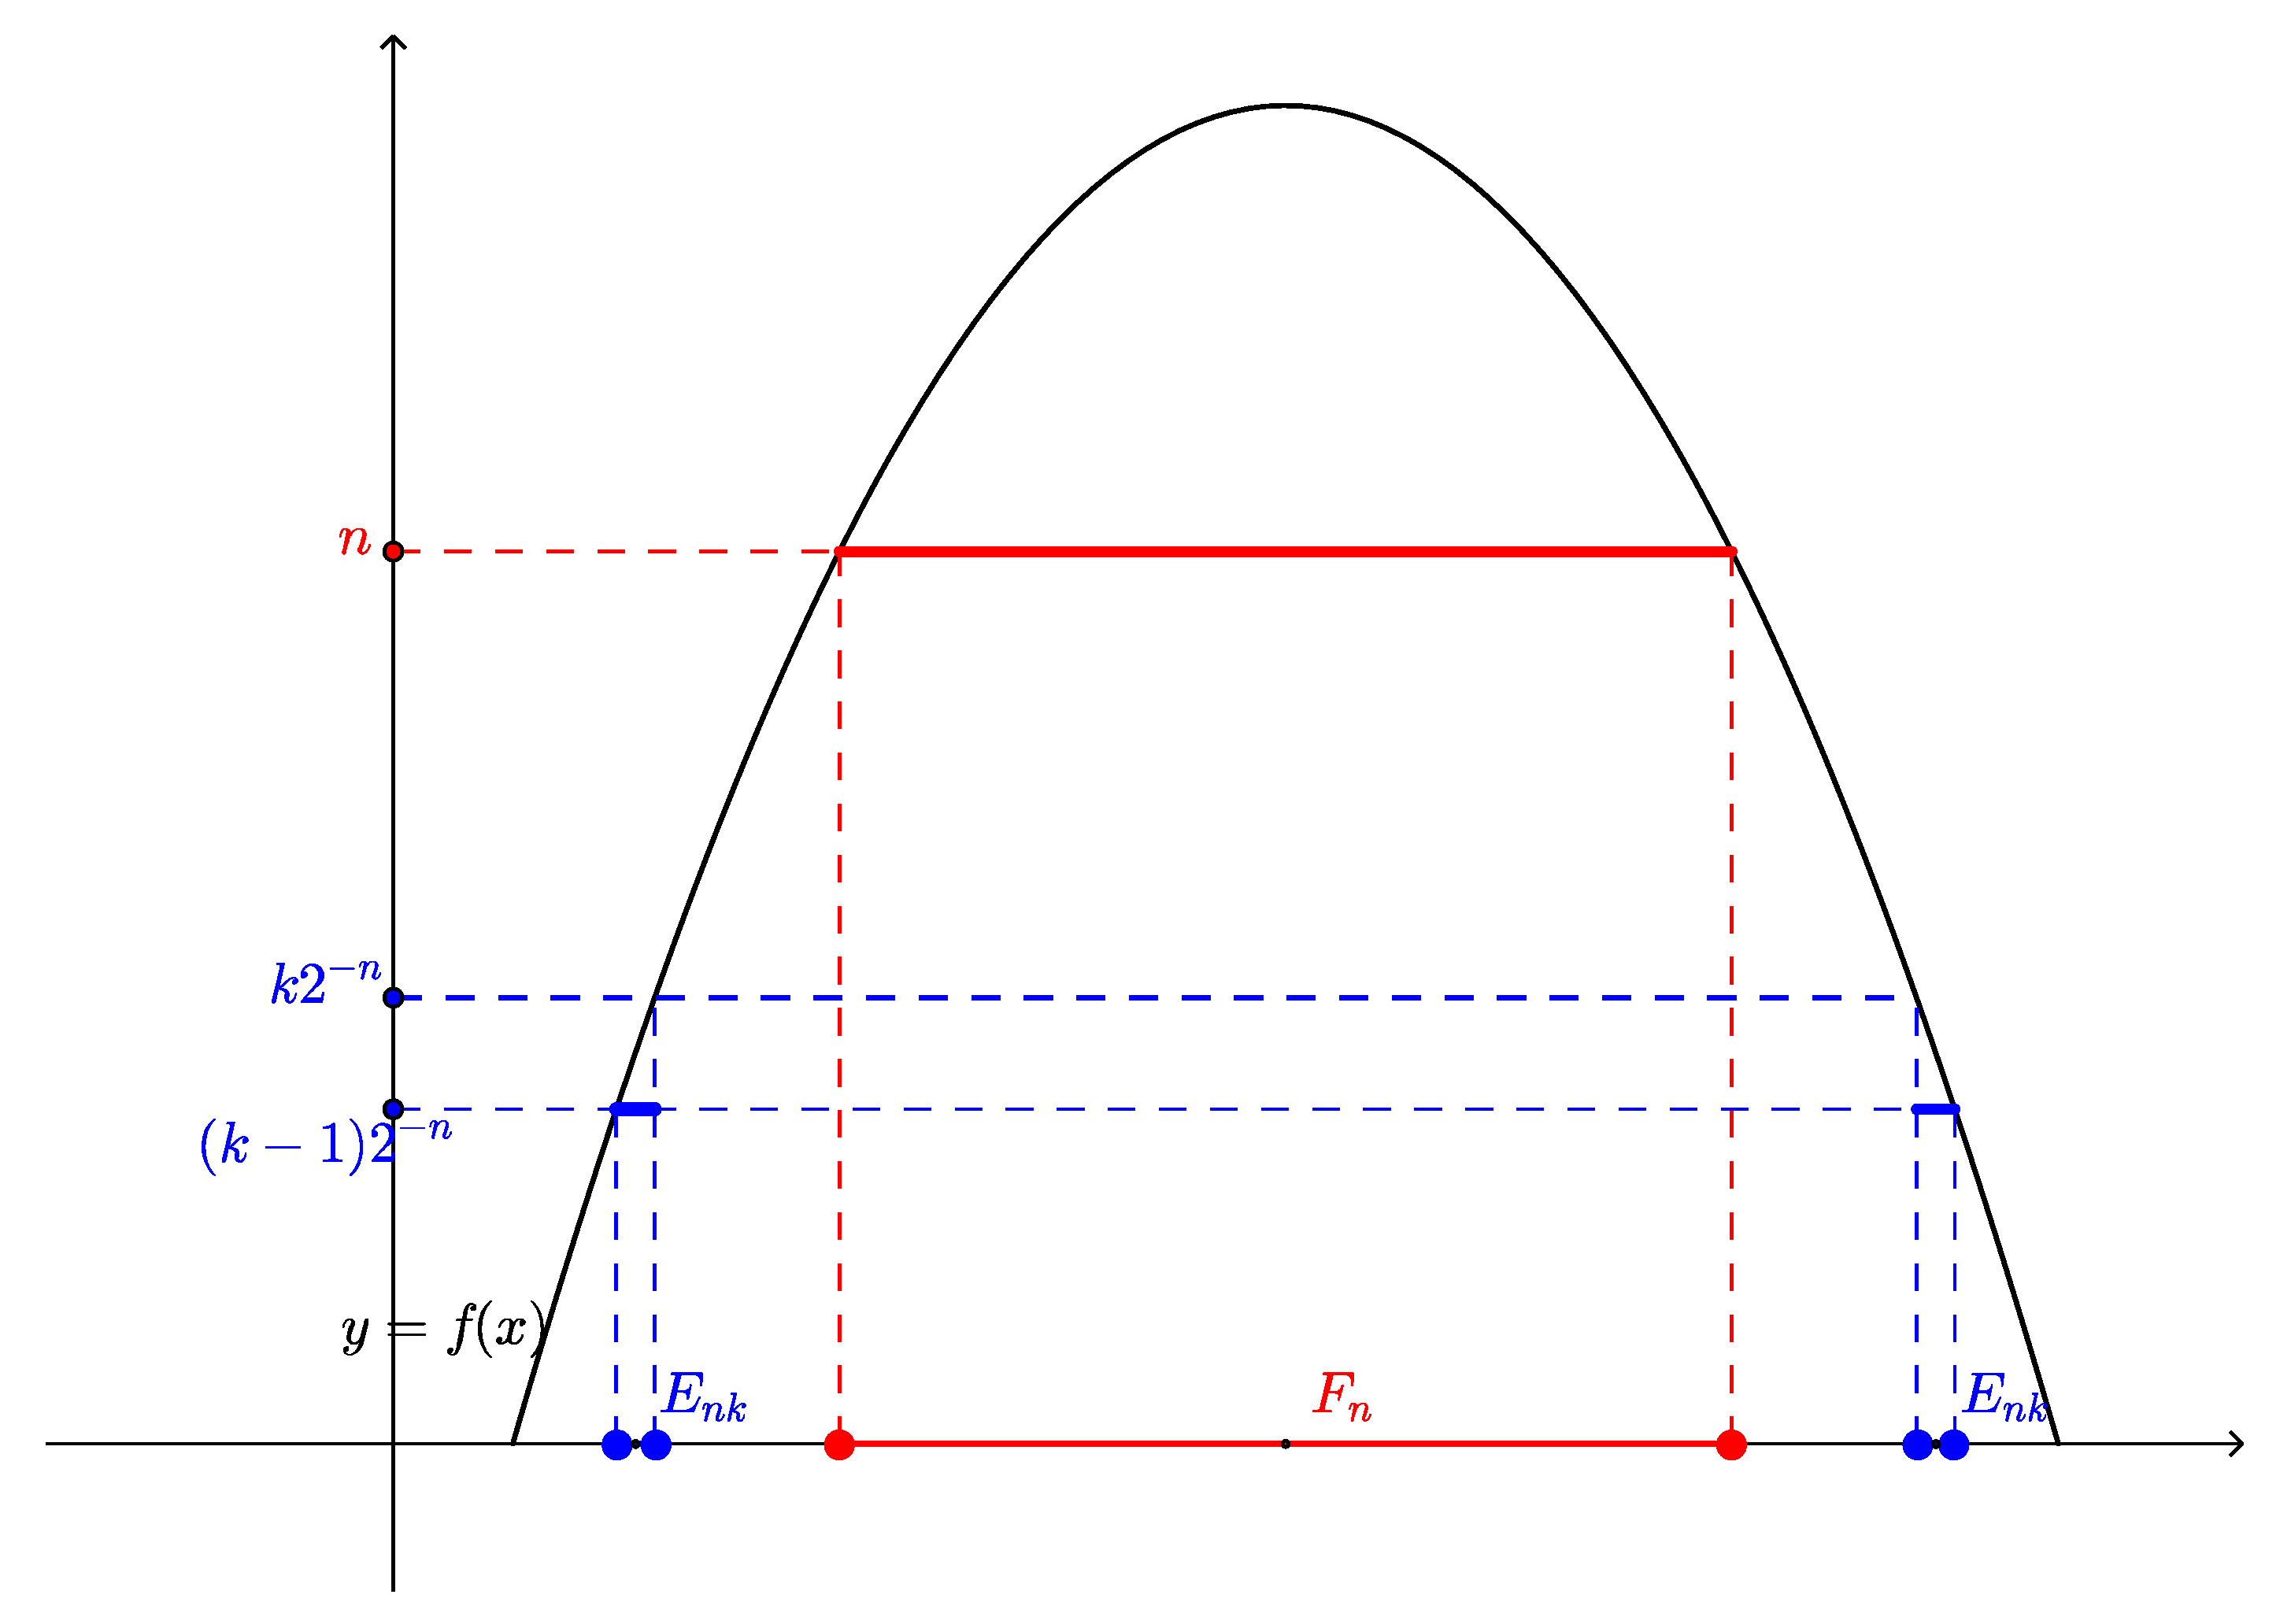
\includegraphics[ext=.pdf,height=13.5\baselineskip]{thLebesgue.pdf}
  \end{center}
  Así, tenemos que:
  \[
    \Omega = F_n \cup \left( \bigcup_{k=1}^{n2^n}E_{n,k} \right)
  \]
  
  y podemos definir las funciones
  \[
    s_n := n\text{\huge {$\chi$}}_{F_n} + \sum_{k=1}^{n2^n}\dfrac{k-1}{2^n}\cdot \text{\huge {$\chi$}}_{E_{n,k}}
  \]
  Además, como $f$ es medible, entonces $F_n$ y $E_{n,k}$ son conjuntos medibles, al ser preimagen de medibles. También tenemos que $s_n$ es medible para cada $n \in \mathbb{N}$ (por serlo $f$ y la función característica de un conjunto), y $s_n(\Omega)$ es finito, por lo que $s_n$ es simple $\forall n \in \mathbb{N}$.

  Ahora, ${s_n}$ es monótona creciente, pues:
      \begin{align*}
 s_{n+1}-s_n =&  \sum_{k=1}^{(n+1)2^{n+1}} \frac{k-1}{2^{n+1}} \text{\huge $\chi$}_{E_{n+1,k}} 
				- \sum_{k=1}^{n2^n} \frac{k-1}{2^n} \text{\huge $\chi$}_{E_{n,k}} 
				\\
			&+	(n+1) \text{\huge{$\chi$}}_{F_{n+1}} - n \text{\huge{$\chi$}}_{F_n} 
				\\ %\pause
			=& \sum_{k=1}^{(n+1)2^{n}} \left[ \frac{2k-1}{2^{n+1}} \text{\huge $\chi$}_{E_{n+1,2k}} 
									+ \frac{(2k-1)-1}{2^{n+1}} \text{\huge $\chi$}_{E_{n+1,2k-1}}  \right]
									\\
			&
				- \sum_{k=1}^{n2^n} \frac{k-1}{2^n} \text{\huge $\chi$}_{E_{n,k}} 
				+	(n+1) \text{\huge{$\chi$}}_{F_{n+1}} - n \text{\huge{$\chi$}}_{F_n}
				\\
%				\pause
			\geq& \sum_{k=1}^{(n+1)2^{n}} \frac{k-1}{2^{n}} \left[  \text{\huge $\chi$}_{E_{n+1,2k}} 
									+ \text{\huge $\chi$}_{E_{n+1,2k-1}}  \right]
%									\\
%			&
				- \sum_{k=1}^{n2^n} \frac{k-1}{2^n} \text{\huge $\chi$}_{E_{n,k}} 
				\\
				&+	(n+1) \text{\huge{$\chi$}}_{F_{n+1}} - n \text{\huge{$\chi$}}_{F_n}
				\\
				\geq& \sum_{k=1}^{n2^{n}} \frac{k-1}{2^{n}} \left[  \text{\huge $\chi$}_{E_{n+1,2k}} 
									+ \text{\huge $\chi$}_{E_{n+1,2k-1}}  \right]
				- \sum_{k=1}^{n2^n} \frac{k-1}{2^n} \text{\huge $\chi$}_{E_{n,k}} 
				\\
				+&\sum_{k=1+n 2^n}^{(n+1)2^{n}} \frac{k-1}{2^{n}} \left[  \text{\huge $\chi$}_{E_{n+1,2k}} 
									+ \text{\huge $\chi$}_{E_{n+1,2k-1}}  \right]
				+	(n+1) \text{\huge{$\chi$}}_{F_{n+1}} - n \text{\huge{$\chi$}}_{F_n}
                                \\
                                = & \sum_{k=1+n 2^n}^{(n+1)2^{n}} \frac{k-1}{2^{n}} \left[  \text{\huge $\chi$}_{E_{n+1,2k}} 
									+ \text{\huge $\chi$}_{E_{n+1,2k-1}}  \right]
				+	(n+1) \text{\huge{$\chi$}}_{F_{n+1}} - n \text{\huge{$\chi$}}_{F_n}
 \end{align*}

Donde la última igualdad se obtiene usando que $E_{n+1, 2k} \cup E_{n+1, 2k-1}=E_{n,k}$. Ahora, usando que $(k-1)2^{-n} \geq n$ para $k=1+n 2^n, 2+n 2^n,\dots n 2^{n+1}$ y que
\[
 \left( E_{n+1, 2(1+n2^n)-1} \cup E_{n+1, 2(1+n2^n)}  \right)
 \bigcup
 \left(E_{n+1, 2(2+n2^n)-1} \cup E_{n+1, 2(2+n2^n)} \right)
 \bigcup \
 \dots
\]
\[
 \dots \
 \bigcup
 \left( E_{n+1, (1+n)2^{n+1}-1} \cup E_{n+1, (1+n)2^{n+1}} \right) 
 =F_{n} \setminus F_{n+1},
\]

tenemos que $\displaystyle s_{n+1}-s_n \geq  n \text{\huge{$\chi$}}_{F_{n}\setminus F_{n+1}}+ (n+1) \text{\huge{$\chi$}}_{F_{n+1}} - n \text{\huge{$\chi$}}_{F_n} \geq 0$.


Probamos para acabar que $\{ s_n(\omega)\} \to f(\omega) \ \ \forall \omega\in\Omega$. En efecto, sea $\omega\in\Omega$ fijo. 
 \begin{itemize}
 \item Si $f(\omega)=\infty \implies \omega\in F_n, $ $\forall n\in \mathbb N$
 \[
 \implies s_n(\omega) =\sum_{k=1}^{n2^n} \frac{k-1}{2^n} \text{\huge{$\chi$}}_{E_{n,k}}(\omega) + n \cdot1\geq n\longrightarrow \infty .
 \]
 \item Si $f(\omega)<\infty \implies \exists n_0\in\mathbb N$ tal que $f(\omega)< n_0$ y $\omega\not\in F_n$ $\forall n\geq n_0$.
 \[
 \begin{aligned}
\implies& \forall n\geq n_0 \ \ \exists ! \ k= 1,2,\dots,n2^n : \frac{k-1}{2^n} \leq f(\omega) < \frac{k}{2^n}
\\
 \implies& s_n(\omega) = \frac{k-1}{2^n} = \frac{E(2^n f(\omega)+1)-1}{2^n} \longrightarrow f(\omega),
 \end{aligned}
  \]
porque $\displaystyle 0\leq f(\omega) - s_n(\omega) = f(\omega) - \frac{E(2^n f(\omega)+1)-1}{2^n} \le \left(\text{Usamos } x-1\leq E(x)\right)$\\ $\displaystyle \leq f(\omega) - \frac{2^n f(\omega)-1}{2^n}  = \frac{1}{2^n}\longrightarrow 0$
 \end{itemize}
\vspace{0.5em}
Además, hay convergencia uniforme en el caso $f(\omega) <\infty$.
\end{proof}

\begin{ncor}[Aritmética de funciones medibles positivas] \label{arit_medibles} Sea $\Omega$ un espacio medible, \mbox{$\alpha \in [0,\infty]$}, y $f,g : \Omega \to [0,\infty]$ medibles. Entonces, $f + g, \ fg, \ \alpha f$ son funciones medibles.
\end{ncor}

  \begin{proof}
    Por el \textit{Teorema de aproximación de Lebesgue} sabemos que existe una sucesión $\{s_n\}$ y otra $\{t_n\}$ de funciones simples positivas que convergen de forma creciente a $f$ y $g$, respectivamente. Además, por la \textit{Proposición \ref{propsimples}} sabemos que podemos generar una sucesión $\{s_n+t_n\} \to f+g$ de funciones simples positivas, y por tanto $f+g$ es medible, al ser el límite puntual de funciones medibles (\textit{Proposición \ref{p1}}).
    
    La demostración para $ \alpha f$ y $fg$ es análoga.
  \end{proof}


% --------------------------------------------------------------------------------
% Integral de funciones medibles positivas.
% --------------------------------------------------------------------------------

\subsection{Integral de funciones medibles positivas}

Abordamos ahora el problema de definir una integral asociada a funciones medibles positivas. Para ello, formalizaremos el concepto de \textit{medida}, que nos permitirá asignar a cada conjunto medible un número $m \in [0,\infty]$, que entenderemos como la \textit{medida} de ese conjunto. 

\begin{ndef}[Medida]
  Si $(\Omega, \mathscr A)$ es un espacio medible, una medida (positiva) es una función $\mu: \mathscr A \rightarrow [0, \infty]$ verificando:
  \begin{nlist}
  \item $\mu(\emptyset) = 0$
  \item \textit{(Aditividad).} $\forall \{A_k\} \subseteq \mathscr A$ con $A_k\cap A_j = \emptyset,\ k \neq j,$ se tiene que:
    $$\mu \left( \bigcup_{k=1}^\infty A_k \right) = \sum_{k=1}^\infty \mu(A_k) $$
  \end{nlist}
  La terna $(\Omega, \mathscr A, \mu)$ se llama \textbf{espacio de medida}.
\end{ndef}

\begin{nprop}[Propiedades de una medida] \label{prop_medida} Si $(\Omega, \mathscr A, \mu)$ es un espacio de medida, se verifican las siguientes propiedades:
  \begin{nlist}
  \item (Monotonía). Si $A,B \in \mathscr A,\ A \subseteq B \implies \mu(A) \leq \mu(B)$
  \item (Subaditividad). $\forall \{A_k\} \subseteq \mathscr A$, se tiene:
    \[
      \mu\left( \bigcup_{k=1}^\infty A_k \right) \leq \sum_{k=1}^\infty \mu(A_k)
    \]
  \item $\forall \{A_k\} \subseteq \mathscr A$ tal que $A_1\subseteq A_2\subseteq \cdots \subseteq A_k \subseteq \cdots,$ se tiene:
    $$\mu \left( \bigcup_{k=1}^\infty A_k \right) = \lim_{k \to \infty}\mu(A_k)$$
  \item $\forall \{A_k\} \subseteq \mathscr A$ tal que $A_1\supseteq A_2\supseteq \cdots \supseteq A_k \supseteq \cdots,$ si $\mu(A_1) < \infty$ se tiene:
    $$\mu \left( \bigcap_{k=1}^\infty A_k \right) = \lim_{k \to \infty}\mu(A_k)$$
  \end{nlist}
\end{nprop}

\begin{proof}\hfill 
\begin{nlist}
    \item Escribimos convenientemente el conjunto B, y aplicamos la definición de medida:
$$B= ( B\setminus A) \cup A \Longrightarrow \mu(B)= \mu ( (B\setminus A) + \mu(A)) \geq \mu(A)	$$
\item Sabemos que si los conjuntos $A_k$ son disjuntos se da la igualdad. Si no lo son,  podemos considerar los conjuntos:
$$B_1=A_1, \ B_2=A_2\setminus B_1, \dots , B_n=A_n \setminus B_{n-1}, \dots $$

Entonces, $\bigcup_{k=1}^\infty B_k = \bigcup_{k=1}^\infty A_k$, con $B_k$  disjuntos dos a dos. Por la propiedad $(i)$,  $\mu (B_k) \leq \mu (A_k)$, y tenemos 

  $$\mu \left( \bigcup_{k=1}^\infty A_k \right) = \mu \left( \bigcup_{k=1}^\infty B_k \right) = \sum_{k=1}^\infty \mu(B_k) \leq \sum_{k=1}^\infty \mu(A_k)$$
\end{nlist}
\end{proof}
  %%% TODO: COMPLETAR DEMOSTRACIÓN -------------------------------------------


\begin{ejemplo}[Medida contadora]
\[ 
 \mu: 2^\Omega\longrightarrow [0,\infty] , \
 \mu (A) = \left\{ \begin{array}{ll}
                               \text{card\,} A , & \text{ si } A \text{ es finito,}
                               \\
                               \infty , &  \text{ si } A \text{ es infinito.}
                              \end{array}
                              \right.
 \]
 
 Es claro que $\mu(\emptyset) = |\emptyset| = 0$, y si $A_k \cap A_j = 0$, se tiene que $\mu(A_k \cup A_j) = |A_k| + |A_j| = $\\ $= \mu(A_k) + \mu(A_j)$. Si alguno de ellos no es finito, la suma será $\infty$ por la aritmética definida en $[0,\infty]$.
	
\end{ejemplo}

\begin{ejemplo}[Medida de Dirac]
Sea $(\Omega,\ \mathscr A=2^\Omega)$ un espacio medible. Para $\omega\in\Omega$, la medida de Dirac  o masa puntual (point mass) es la medida $\delta_\omega:\mathscr A \longrightarrow [0,\infty ]$ dada por 
 \[
 \delta_\omega (A) = \left\{ \begin{array}{ll}
                                1, & \text{ si } \omega\in A,
                               \\
                               0 , &  \text{ si } \omega\not\in A.
                              \end{array}
                              \right.
 \]
 
 Fijemos $\omega \in \Omega$. Claramente $\delta_\omega(\emptyset) = 0$, porque el conjunto vacío no contiene ningún punto. Ahora, si $A_k \cap A_j = \emptyset$, pueden darse dos casos:
 
\begin{itemize}
    \item $\omega \in A_k\cup A_j \implies \omega \in A_k$ o bien $\omega \in A_j$. Supongamos $\omega \in A_k$. Entonces, $\delta_\omega(A_k\cup A_j) = 1 = 1 + 0 = \delta_\w(A_k) + \delta_\w(A_j)$.
    \item $\w \notin A_k\cup A_j \implies \w \notin A_k$ y $\w \notin A_j$. Entonces, $\delta_\omega(A_k\cup A_j) = 0 = 0 + 0 =\delta_\w(A_k) + \delta_\w(A_j)$.
\end{itemize}
	
\end{ejemplo}

\begin{ejemplo}[Medida de Lebesgue]
	 Si $(\Omega = \mathbb R^N, \mathscr A= \mathcal B(\mathbb R^N))$ espacio medible, la medida de Lebesgue es $\lambda: \mathscr A \to [0,\infty]$ dada por  
 \[
 \lambda ([a_1,b_1]\times  [a_2,b_2]\times \dots [a_N,b_N]) = (b_1-a_1) (b_2-a_2) \dots (b_N-a_N)
 \]
\end{ejemplo}

Estamos ya en disposición de definir lo que entenderemos por integral de una función medible positiva, en el marco de un espacio de medida $(\W, \mathscr A, \mu)$. Como ya dijimos, el problema se reducirá a estudiar integrales asociadas a funciones simples, las cuales definimos a continuación.

\begin{ndef}[Integral de función simple positiva]
  Si $E \in \mathscr A$ y $s:\Omega \to [0,\infty)$ es simple, i.e, $\displaystyle s= \sum_{k=1}^n \alpha_k \rchi_{A_k}$, entonces definimos la integral de $s$ en $E$ como: 
  \[
    \int_E s\, d\mu := \sum_{k=1}^n \alpha_k \mu(E\cap A_k)
  \]
\end{ndef}

Comprobemos ahora que la definición es consistente, es decir, que el valor de la integral no depende de la representación de $s$. Sea $s = \sum_{j=1}^m \beta_j \rchi_{B_j}$ con $\{B_j\}_{j=1}^m$ medibles y disjuntos, y $\{\beta_1,\dots,\beta_m\} \subseteq [0,\infty)$. Sabemos por la \textit{Proposición \ref{caract_simples}} que $s$ es simple. Además, supongamos que $s= \sum_{k=1}^n \alpha_k \rchi_{A_k}$ es su descomposición canónica.

Observemos que puede ocurrir que $\beta_i = \beta_j$ para algún $i\neq j$. Teniendo esto en cuenta, definimos $I_k := \{j \in \{1,\dots,m\} : \beta_j = \alpha_k\}$, y entonces $$A_k = \bigcup_{j\in I_k} B_j$$ Realizando transformaciones algebraicas, tenemos que $$\sum_{j=1}^m \beta_j\mu(E \cap B_j) = \sum_{k=1}^n \sum_{j \in I_k} \beta_j \mu(E \cap B_j) = \sum_{k=1}^n \alpha_k \sum_{j \in I_k} \mu(E \cap B_j) \overset{(*)}{=} \sum_{k=1}^n \alpha_k  \mu \left(\bigcup_{j \in I_k} E \cap B_j \right) = $$ 

$$= \sum_{k=1}^n \alpha_k  \mu \left(E \cap\bigcup_{j \in I_k} B_j \right) = \sum_{k=1}^n \alpha_k  \mu (E \cap A_k)$$

donde la igualdad $(*)$ se da por la \textit{aditividad} de $\mu$, teniendo en cuenta que los conjuntos $\{B_j \cap E\}_{j=1}^m$ son disjuntos dos a dos, por serlo $\{B_j\}_{j=1}^m$.

Por tanto, queda probado que $$\displaystyle \int_E s\, d\mu = \sum_{j=1}^m \beta_j \mu(E \cap B_j)$$

%%% TODO: Se puede demostrar que no es necesario que los conjuntos B_j sean disjuntos.

\begin{nprop}[Propiedades integral funciones simples] \label{int_simples} Sea $s$ una función simple. Entonces, se verifica lo siguiente:
\vspace{0.5em}
    \begin{nlist}
    \item $\displaystyle \int_E \alpha s\, d\mu = \alpha \int_E s\, d\mu, \quad \forall \alpha \in [0,\infty]$
    \item Si $A,B$ son dos conjuntos medibles y disjuntos, entonces $$\int_{A \cup B} s\, d\mu = \int_A s\,d\mu + \int_B s\, d\mu$$
    \item Si $t$ es simple y $\displaystyle s(\omega) \leq t(\omega)\ \forall \w \in \W$, entonces $\displaystyle \int_E s\, d\mu \leq \int_E t\, d\mu$
    \end{nlist}
\end{nprop}

\begin{proof} Supongamos que $\displaystyle s = \sum_{k=1}^n \alpha_k\rchi_{A_k}$ (descomposición canónica).\hfill
    \begin{nlist}
	\item Sabemos que $\alpha s$ es una función simple, por ser producto de una simple y un escalar. De hecho, $\displaystyle \alpha s = \sum_{k=1}^n \alpha \alpha_k \rchi_{A_k}$. Entonces, se tiene que: $$\int_E \alpha s\, d\mu = \sum_{k=1}^n \alpha \alpha_k \mu (E\cap A_k) = \alpha \sum_{k=1}^n \alpha_k \mu (E\cap A_k) = \alpha \int_E s\, d\mu$$
	\item Basta observar lo siguiente: $$\int_{A\cup B} s\, d\mu = \sum_{k=1}^n \alpha_k\cdot \mu((A\cup B)\cap A_k) = \sum_{k=1}^n \alpha_k \cdot \mu((A\cap A_k)\cup (B \cap A_k)) \overset{(*)}{=}$$ $$=\sum_{k=1}^n \alpha_k \left( \mu(A\cap A_k) +  \mu(B \cap A_k)\right) = \sum_{k=1}^n \alpha_k \mu(A\cap A_k) + \sum_{k=1}^n \alpha_k \mu(B\cap A_k) =$$ $$= \int_A s\, d\mu + \int_B s\, d\mu,$$ 
	
	donde $(*)$ es consecuencia de la \textit{aditividad} de $\mu$, teniendo en cuenta que $(A\cap A_k)$ y $(B\cap A_k)$ son disjuntos, por serlo $A$ y $B$.
\end{nlist}
\end{proof}
%%% TODO: Completar demostración último apartado

\begin{ndef}[Integral de función medible positiva]
  Si $E\in \mathscr A$ y $f: \Omega \to [0,\infty]$ es medible, entonces definimos la integral de $f$ en $E$ como:
  \[
    \int_E f\, d\mu := \sup\left\{\int_E s\, d\mu: \text{ $s$ es simple positiva}, \ s \leq f\right\}
  \]
  
\end{ndef}

Veamos ahora un teorema importante que, dada una sucesión de funciones convergente, nos permite bajo ciertas condiciones ``intercambiar la integral con el límite''. Antes, necesitaremos el siguiente


\begin{lema} \label{phi}
	Sea $s:\W \to [0,\infty)$ simple. Entonces, $\varphi:\mathscr A \to [0,\infty]$ dada por $$\varphi(E) = \int_E s\, d\mu, \quad \forall E \in \mathscr A$$ es una medida.
\end{lema}

	\begin{proof} En primer lugar, es claro que $\displaystyle \varphi(\emptyset) = \int_\emptyset s\, d\mu = 0$, pues $\mu$ es una medida, y $\mu(\O) = 0$. Por otro lado, dada una sucesión $\{E_k\}$ de conjuntos medibles y disjuntos, se tiene que $$\varphi \left(\bigcup_{k=1}^\infty E_k \right) = \int_{\bigcup_{k=1}^\infty E_k} s\, d\mu \overset{(*)}{=} \sum_{k=1}^\infty \int_{E_k} s\, d\mu = \sum_{k=1}^\infty \varphi(E_k),$$ 
	
	donde $(*)$ es consecuencia de la \textit{Proposición \ref{int_simples} ii}. Por tanto, $\varphi$ es aditiva, luego es una medida.
	    %%% TODO: Estilo de referencias a un apartado en específico de una proposición.
\end{proof}

\begin{nth}[Teorema de la convergencia monótona] \label{tcm}
  Sea $(\Omega,\mathscr A,\mu)$ un espacio de medida. Sea $E\in \mathscr A$ y $f_n: \Omega \to [0,\infty]$ medibles. Supongamos que $f_n(\omega) \leq f_{n+1}(\omega) \, \ \forall \omega \in \Omega$. Entonces:
  \[
    \int_E \lim_{n \to \infty} f_n\ d\mu = \lim_{n \to \infty}\int_E f_n\, d \mu
  \]
\end{nth}

  \begin{proof} Empezamos observando que $\displaystyle f(\omega):= \lim _{n\to \infty} f_n(\omega)$ es medible por la \textit{Proposición \ref{p1}}, teniendo en cuenta que $\{f_n(\omega)\}$ es monótona creciente, y por tanto convergente. Veamos ahora las dos desigualdades.

    \boxed{\geq} Como $f_n \leq f_{n+1} \leq f$ por hipótesis, tenemos que:
    \[
    \left\{ s  : \begin{array}{r} \text{ $s$ simple positiva}\\
        s \leq f_n 
      \end{array}\right\}  \subseteq \left\{ s: \begin{array}{r} \text{ $s$ es simple positiva}\\
        s\leq f_{n+1}
	
      \end{array} \right\} \subseteq \left\{s: \begin{array}{r}\text{ $s$ es simple positiva}\\ s \leq f
	
      \end{array}\right\}
    \]
    Tomando supremos de las respectivas integrales, esto implica que:
    \[
      \int_E f_n\, d \mu \leq \int_E f_{n+1}\, d\mu \leq \int_E f\, d \mu \implies \exists \lim_{n\to \infty} \int_E f_n\, d\mu \leq \int_E f\, d \mu
    \]
    \boxed{\leq} Como
    \[
      \int_E f\, d \mu = sup \left\{\int_E s\, d\mu : \begin{array}{r} \text{ $s$ es simple positiva}\\
        s \leq f
	
      \end{array}\right\}
    \]
    basta ver que
    \[
      \begin{rcases}
	\text{ $s$ es simple positiva}\\
	s \leq f
      \end{rcases} \implies \int_E s\, d\mu \leq \lim_{n\to \infty} \int_E f_n\, d\mu,
    \]
    pues al tomar el supremo de la primera integral, se mantiene el orden y tendríamos lo buscado. Vamos a probar este hecho. Sea $s: \Omega \to [0,\infty)$ simple positiva tal que $s \leq f$. Fijamos $\rho \in (0,1)$, y para cada $n \in \mathbb{N}$ definimos
    \[
      E_n := \{\omega \in E : \rho s(\omega) \leq f_n(\omega)\} 
    \]
    Tenemos que los conjuntos $E_n$ son medibles, puesto que la función $h:= f_n -\rho s$ es medible, y por tanto $E_n = h^{-1}([0,\infty))$ es medible para cada $n \in \mathbb{N}$. Además, claramente $E_n \subseteq E_{n+1} \ \forall n \in \mathbb{N}$, pues $\fn$ es creciente, y se verifica que $$E = \bigcup_{n=1}^\infty E_n$$ Para verlo, sea $\w \in E$. Si $f(\w) = 0 \implies s(\w) = 0 \implies \w \in E_1$. En otro caso, $\rho s(\w) < f(\w)$, pues $\rho < 1$. Entonces, $\exists n \in \mathbb{N}: \w \in E_n$. 
    %%% TODO: La función h es medible, pero no positiva. Arreglar
    Ahora, se tiene lo siguiente, donde $\varphi$ es la medida definida en el \textit{Lema \ref{phi}}:
    \begin{equation} \label{eq1}
      \rho\varphi(E_n) = \rho \int_{E_n} s\, d\mu = \int_{E_n} \rho s\, d \mu \overset{\text{def. $E_n$}}{\leq} \int_{E_n}f_n\, d\mu \leq \int_E f_n\, d\mu
    \end{equation}
    %%% WARNING: ¿estamos usando sin demostrarlo que \rho s <= f_n \implies \int \rho s <= \int f_n ??? 
    La última desigualdad es así porque para toda función simple $s \leq f_n$ se tiene que $\int_{E_n}s\,d\mu \leq \int_E s\, d \mu$, como consecuencia de que $E_n \cap A_k \subseteq E \cap A_k$ y la monotonía de $\mu$.

    Ahora, como $\varphi$ es una medida, si $n \to \infty$ en \eqref{eq1}, entonces: 
    $$\rho \varphi(E) =  \rho\int_E s\, d\mu \implies \rho \int_E s\,d\mu \leq \lim_{n\to \infty}\int_E f_n\, d\mu$$ Donde hemos usado que $\varphi(E_n) \to \varphi(E)$ cuando $n\to\infty$, porque $\{E_n\}$ es una sucesión encajada de conjuntos medibles, y $\varphi$ es una medida (\textit{Proposición \ref{prop_medida} iii}).
    Por último, hacemos tender $\rho\to 1$, y concluimos la prueba:
    \[
     \int_E s\, d\mu \leq \lim_{n\to \infty}\int_E f_n\, d\mu
    \]
  \end{proof}

Una vez que conocemos el \textit{teorema de la convergencia monótona}, podemos deducir una serie de propiedades útiles sobre la integral de funciones medibles positivas. Por comodidad, abreviaremos dicho teorema como $T.C.M$.

\begin{nprop}[Propiedades integral funciones medibles positivas] \label{int_medibles}
Sean \\ $f,g:\Omega \to [0,\infty]$ medibles positivas, $\alpha \in \R, E \in \mathscr A$. Entonces, se verifican las siguientes propiedades.

\begin{nlist}
\item Linealidad de la integral
  \[
    \int_E (f+g)\, d\mu = \int_E f\, d\mu + \int_E\, g d\mu
  \]
  \[
    \int_E \alpha f\, d\mu = \alpha \int_E f\, d\mu
  \]
  
\item Monotonía $$g(\omega) \leq f(\omega) \ \forall \omega \in \Omega \implies \int_E g\, d\mu \leq \int_E f\, d \mu$$
  
  %%% TODO: revisar nombre de la propiedad
\item Integración en un conjunto más grande $$\int_E f\, d \mu =  \int_\Omega f\rchi_E \,d\mu$$

\item Condiciones suficientes para que la integral sea nula $$\mu(E) = 0 \implies \int_E f\, d\mu = 0$$ $$f(\w) = 0 \ \ \forall \w \in \W \implies \int_E f\,d\mu = 0$$
\end{nlist}
\end{nprop}

\begin{proof}\hfill
\begin{nlist}
    \item Ya sabemos por el \textit{Corolario \ref{arit_medibles}} que $f+g$, $fg$ y $\alpha f$ son medibles. 
    $$\dots$$
    Recordemos que tomamos el convenio $\alpha \cdot \infty = \infty, \ \alpha \cdot 0 = 0$.
    
    \item
    \item
    \item Veamos la primera implicación. Empezamos notando que si $\mu(E) = 0$, entonces $\int_E s\,d\mu = 0$ para toda función simple $s$. En efecto, si $s = \sum_{k=1}^n \alpha_k \rchi_{A_k}$ es su forma canónica, entonces: $$\int_E s\,d\mu = \sum_{k=1}^n \alpha_k \mu(E \cap A_k) = \sum_{k=1}^n \alpha_k \cdot 0 = 0,$$ donde hemos usado que $\mu(E\cap A_k) = 0\ \forall k \in \{1,\dots,n\}$ por la monotonía de $\mu$, notando que $E\cap A_k \subseteq E$.
    
    Por tanto, $\displaystyle \sup\left\{\int_E s\,d\mu : s \text{ es simple positiva, } s \le f \right\} = 0$, y hemos acabado.
    
    Para la segunda implicación, observemos que $f=0$ es simple, pues el único valor que toma es el 0. Por tanto: $$\int_E f\,d\mu =  \sum_{k=1}^n 0\cdot \mu(E) = 0$$
\end{nlist}
\end{proof}
%%% TODO: Completar demostración.

\begin{nprop} \label {phi_2} Sea $f:\W \to [0,\infty]$ medible. Entonces, $\varphi:\mathscr A \to [0,\infty]$ dada por $$\varphi(E) = \int_E f\, d\mu, \quad \forall E \in \mathscr A$$
es una medida. Además, se verifica lo siguiente:
  \begin{nlist}
  \item $E\in \mathscr A, \ \mu(E) = 0 \implies \varphi(E) = 0$
  \item $g:\Omega \to [0,\infty]$ medible $\displaystyle \implies \int_E g\, d\varphi = \int_E g f\, d\mu$
  \end{nlist}
%%% TODO: completar
\end{nprop}

Para finalizar este apartado, veamos dos teoremas importantes, ambos consecuencia directa del \textit{teorema de la convergencia monótona}.

\begin{nth}[Teorema de Levi] Sean $f_n: \Omega \to [0,\infty]$ medibles. Entonces
\[
     \int_E \sum_{n=1}^\infty f_n\, d \mu = \sum_{n=1}^\infty \int_E f_n\, d\mu
  \]
\end{nth}

	  \begin{proof} \hfill \\
    Si $f_n:\Omega \to [0,\infty]$ son medibles y $\sum_{n\geq 1}f_n$ una serie de funciones, definimos las sumas parciales como
    \[
      S_k= \sum_{n=1}^k f_n, \quad \forall k \in \mathbb{N}
    \]
    Tenemos que $S_1 \leq \cdots \leq S_k \leq S_{k+1} \leq \cdots $, es decir, $S_k$ es monótona creciente. Además, las funciones $S_k$ son medibles para cada $k \in \mathbb{N}$, por ser suma de funciones medibles. Aplicando el \hyperref[tcm]{\textit{T.C.M}}, tenemos que:
    \[
      \lim_{k \to \infty} \int_E S_k\, d\mu = \int_E \lim_{k\to \infty} S_k\, d\mu \implies \lim_{k \to \infty} \int_E \sum_{n=1}^k f_n\, d\mu = \int_E \sum_{n=1}^\infty f_n \overset{\text{Proposición \ref {int_medibles}} \ i}\implies
    \]
    
    \[
    \implies \lim_{k\to\infty} \sum_{n=1}^k \int_E f_n\,d\mu = \int_E \sum_{n=1}^\infty f_n\,d\mu \implies \sum_{n=1}^\infty \int_E f_n\,d\mu = \int_E \sum_{n=1}^\infty f_n\,d\mu
    \]
\end{proof}

\begin{lema} [Lema de Fatou]
  Si $(\Omega,\mathscr A,\mu)$ es un espacio de medida, $E\in \mathscr A$ y tenemos funciones $f_n:\Omega \to [0,\infty]$ medibles, entonces:
  \[
    \int_E \liminf_{n \to \infty} f_n\, d\mu \leq \liminf_{n\to \infty} \int_E f_n\, d\mu
  \]
\end{lema}

  \begin{proof} Definimos $g_k(\omega) :=  \underset{n\geq k}{\text{inf\,} } f_n(\omega )$. Sabemos que $\{g_k\}$ es monótona creciente por definición, y además es una sucesión de funciones medibles por la \textit{Proposición \ref{p1}}. Entonces, tenemos que: $$\underset{n\to \infty}{\text{lim\,inf\,}} f_n (\omega ) = \underset{k\geq 1}{\text{sup\,}}  \left\{ \underset{n\geq k}{\text{inf\,} } f_n(\omega )\right\}  =  \underset{k\geq 1}{\text{sup\,}} g_k(\omega) = \lim_{k\to\infty} g_k(\w)$$ 
  
Ahora, aplicando el \hyperref[tcm]{\textit{T.C.M}}, se tiene que:
\[
\int_E \underset{n\to \infty}{\text{lim\,inf\,}} f_n\, d\mu  =  \int_E \underset{k\to \infty}{\text{lim}} g_k\, d\mu 
 =  \underset{k\to \infty}{\text{lim}}  \int_E g_k d\mu 
\]

Por último, sabemos que $g_k(\omega)\leq f_k(\omega) \ \forall \omega\in \Omega $ (por definición de ínfimo). Además, se tiene que $g_k \le \inf_{n\ge k}\ f_k$. Aplicamos la monotonía de la integral:
\[
\int_E g_k\, d\mu  \leq \inf_{n\ge k} \int_E f_n\, d\mu 
\overset{k\to\infty}{\implies}
\int_E \underset{n\to \infty}{\text{lim\,inf\,}} f_n\, d\mu 
\leq   \underset{k\to \infty}{\lim \text{inf}} \int_E f_k\, d\mu
\]
%%% WARNING: Por qué está completa la prueba poniendo solo \lim en lugar de \liminf en la última desigualdad?
\end{proof}

\subsection{Integral de funciones medibles}

%%% FIXME: FALTAN COSAS


\begin{nth}[Convergencia dominada de Lebesgue]
  Sean $f_n : \Omega \rightarrow \R$ funciones medibles y $E \in \mathscr A$. Además, supongamos que ${f_n(\omega)} \rightarrow f(\omega)$ c.p. con $\omega \in E$. Finalmente, supongamos que $\exists g: \Omega \rightarrow \R$ integrable tal que $|f_n(\omega)| \leq g(\omega) \ \forall \omega \in E$. Entonces,
  
  $$ \lim_{n \to \infty} \int_E f_n d \mu = \int_E  \left( \lim_{n \to \infty} f_n \right) d \mu$$ 
\end{nth}

\begin{nota}
  Como para cada $n$, $|f_n| \leq g$ y $g$ es integrable, $|f_n|$ también es integrable, luego cada $f_n$ es integrable.
\end{nota}

\begin{nota}
  Como $f(\omega) = \lim_{n \to \infty} f_n(\omega)$ con cada $f_n$ una función medible $\Rightarrow f$ es medible en $\Omega$.
\end{nota}

\begin{proof}
  Definimos $g_n(\omega) := 2g(\omega)\rchi_E(\omega) - \abs{f_n(\omega) - f(\omega)} \chi_E (\omega)$, que es integrable. Es claro que $\{g_n(\omega)\} \rightarrow 2g(\omega)\rchi_E(\omega)$, ya que $f_n(\omega) \rightarrow f(\omega)$ y $\rchi_E$ es acotada.
  
  Vamos a ver además que $g_n \geq 0$ y es medible en $\Omega$ porque $$|f_n - f| \leq |f_n| + |f| \leq g + g = 2g\rchi_E(\omega)$$
  Por el \textit{Lema de Fatou}, 
  $$\liminf_{n \to \infty} \int_{\Omega} g_n d \mu \geq \int_{\Omega} \liminf_{n \to \infty} g_n d \mu = 2 \int_{\Omega} g\rchi_E(\omega)d\mu$$
  
  $$\liminf_{n \to \infty} \left[\int_{\Omega} 2g(\omega)\rchi_E(\omega) d\mu - \int_{\Omega} \abs{f_n(\omega) - f(\omega)}\rchi_E(\omega) d \mu \right] \leq 2\int_{\Omega} g\rchi_E(\omega) d \mu$$

  Como recordatorio, $$\text{si } \exists \lim_{n \to \infty} x_n \text{ entonces } \liminf_{n \to \infty} (x_n + y_n) = \lim_{n \to \infty} x_n + \liminf_{n \to \infty} y_n$$ Además, $$\liminf_{n \to \infty} x_n = - \limsup_{n \to \infty} (- x_n)$$
  Luego entonces
  
  $$2 \int_{\Omega} g(\omega)\rchi_E(\omega) d \mu + \liminf_{n \to \infty} \left[-\int_{\Omega} \abs{f_n - f} \rchi_E(\omega) d \mu \right]$$
  
  $$ = 2 \int_{\Omega} g \rchi_E(\omega) d \mu - \limsup_{n \to \infty} \int_{\Omega} \abs{f_n - f} \rchi_E(\omega) d \mu$$
  
  En resumen,
  
  $$2 \int_{\Omega} g \rchi_E(\omega) d \mu - \limsup_{n \to \infty} \int_{\Omega} \abs{f_n - f} \rchi_E(\omega) d \mu \geq 2 \int_{\Omega} g \rchi_{E} d \mu$$
  
  $$\int_{\Omega} g \rchi_{E} d \mu = \int_{\Omega} g  d \mu < \infty \Rightarrow \limsup_{n \ to \infty} \int_{\Omega} \abs{f_n - f} \rchi_E d \mu \leq 0$$
  
  $$\Rightarrow 0 \leq \liminf_{n \to \infty} \int_{\Omega} \abs{f_n - f} \rchi_E d \mu \leq \limsup_{n \to \infty} \int_{\Omega} \abs{f_n - f} \rchi_E d \mu = 0$$
  
  $$\Rightarrow \exists \lim_{n \to \infty} \int_{\Omega} \abs{f_n - f} \rchi_E d \mu = 0$$
  
  Sustituyendo $\Omega$  por $E$ hemos probado entonces que 
  $$\lim_{n \to \infty} \int_{E} \abs{f_n - f} d \mu = 0$$
  
  $$- \int_E \abs{f_n - f} d \mu \leq \int_E (f_n - f) d \mu \leq \int_E \abs{f_n - f} d \mu$$
  
  Sumando entonces $\displaystyle \int_E f d \mu$ a cada término tenemos
  
  $$ - \int_E \abs{f_n - f} d \mu + \int_E f d \mu \leq \int_E f_n d \mu \leq \int_E \abs{f_n - f} d \mu + \int_E f d \mu$$
  
  Y si finalmente, tomando $\lim_{n \to \infty}$ tenemos que
  $$ \exists \lim_{n \to \infty} \int_E f_n d \mu = \int_E f d \mu$$
\end{proof}

Una vez que tenemos estos resultados, vamos a trabajar un poco con ellos para acuñarlos. Comenzaremos con el Lema de Fatou.

\begin{nprop}[Lema de Fatou para funciones medibles]
  Sean $f_n: \omega \to \R$ medibles. Supongamos que $\exists h: \Omega \to \R$ con $-\infty < \int_\Omega h d\mu := \int_\Omega d\mu - \int_\Omega d\mu $ tal que $f_n(\omega) \geq h(\omega) \ \ \ \forall \omega \in \Omega$.\\
  Entonces:
  $$ \lim_{n\to \infty}\int_\Omega f_n d\mu \geq \int_\mu (\liminf_{n\to \infty}f_n )d\mu$$
\end{nprop}
\begin{proof}
  Llamamos $h_n:= f_n - h \geq 0$ y medible por diferencia de funciones medibles. Ahora, usamos el lema de Fatou para funciones medibles positivas y así tenemos que:
  $$ \lim_{n\to \infty} \int_\Omega (f_n -h) d\mu \geq \int_\Omega \liminf_{n\to \infty}(f_n - h) d\mu$$
  
  $$ ( \liminf_{n\to \infty}\int_\Omega f_n d\mu )  - \int_\Omega h d\mu \geq \int_\Omega \liminf_{n\to \infty} f_n d\mu - \int_\Omega f_n d\mu$$
  Y podemos suprimir los miembros iguales y haber probado este resultado.
\end{proof} 

\begin{nth}[Teorema de la convergencia monótona para funciones integrables]
  Sean $f_n: \Omega \to \R$ funciones integrables y $f_n(\omega) \leq f_{n+1} \ \ \ \forall \omega \in \Omega$. Supongamos también que $\{\int_\Omega f_n d\mu\}$ es una sucesión acotada superiormente. Entonces: 
  $$ \begin{cases}
    f(\omega):= \lim_{n\to \infty}f_n(\omega) \text{ es integrable}\\
    \lim_{n \to \infty} \int_\Omega f_n d\mu = \int_{\Omega}\lim_{n\to \infty} f_n d\mu
  \end{cases}$$
  
\end{nth}
\begin{proof}
  Sabemos que $f_1 \leq f_2 \leq \cdots \leq f_n \leq \cdots $. Como queremos que sean positivas, definimos $h_n:= f_n - f_1$, que es medible por diferencia de medibles y monótona creciente. Así, tenemos las condiciones para aplicar el teorema de la convergencia monótona para funciones medibles positivas y ver que:
  $$ \lim_{n \to \infty} \int_\Omega h_n d\mu = \int_\Omega \lim_{n \to \infty}h_n d\mu$$
  Y como la sucesión de las integrales está acotada superiormente, tenemos que:
  $$ +\infty > \lim_{n\to \infty} \int_\Omega f_n d\mu = \int_\Omega f d\mu \geq \int_\Omega f_1 d\mu > -\infty$$
\end{proof}

\begin{nota}
  Estos dos teoremas, los podemos realizar en un $E$ un subconjunto del espacio medible $\Omega$
\end{nota}

%%% WARNING: ¿quitar?
\begin{nprop}
  Sean $f,g: \Omega \to \R$. Si $f$ es medible y $f(\omega) =  g(\omega)$ a. e. $\forall \omega \in \Omega$, entonces $g$ es medible. Además, si $f$ es integrable, $g$ es integrable y $\int_\Omega f d\mu = \int_\Omega g d\mu$.
\end{nprop}

\begin{nprop} Sea $f:\mathscr A \to [0,\infty]$ medible. Entonces, se verifican las siguientes afirmaciones:
  \begin{nlist}
	
  \item $\displaystyle \int_\Omega f\, d\mu < \infty \implies \mu(\{\omega \in \Omega: f(\omega) =  \infty\}) = 0$
  \item $\displaystyle \int_\Omega f\, d\mu = 0 \iff \mu(\{\omega \in \Omega : f(w) > 0\}) = 0$
\end{nlist}
\end{nprop}

    \begin{proof} \hfill
    \begin{nlist}
    \item Llamemos $E := \{\w \in \W: f(\w) = \infty\} \subseteq \W$. Se tiene que $E$ es medible, pues es diferencia de conjuntos medibles: $E = f^{-1}[0,\infty] \setminus f^{-1}[0,\infty)$. Veamos el contrarrecíproco: $$\int_\W f\, d\mu \ge \int_E f\,d\mu \ge \int_E n\rchi_E\,d\mu = n\mu(E) \quad \forall n \in \mathbb{N}$$
    Como $n\mu(E) \to \infty$ cuando $n\to \infty$, tenemos lo buscado.
    \item Veamos las dos equivalencias:
    
    \boxed{\Rightarrow}  Empezamos probando que si $s$ es una función simple positiva con integral $\int_\Omega s \, d\mu = 0$, entonces $\mu(\{ \omega\in\Omega \, :\, s(\omega) >0\} ) = 0$. En efecto, si $$s(\omega)=\sum_{i=1}^m \alpha_i \text{\Large$\chi$}_{A_i}, \quad (\alpha_1,\alpha_2,\dots,\alpha_m > 0)$$ entonces $\displaystyle A:=\{ \omega\in\Omega \, :\, s(\omega) >0\} = \bigcup_{i=1}^m A_i$, y $\displaystyle \int_\Omega s \, d\mu = \sum_{i=1}^m \alpha_i \mu (A_i) = 0 \implies\mu(A_i)=0\ \forall i=1,\dots , m$, por lo que $\mu(A)=0 $.

Ahora, por el \textit{Teorema de aproximación de Lebesgue} existe una sucesión de funciones simples positivas $\{ s_n(\omega)\}\nearrow f(\omega)$. Por el \textit{Teorema de convergencia monótona}: 

$$0\leq \int_\Omega s_n \, d\mu \nearrow \int_\Omega f\, d\mu = 0,$$

es decir, $\displaystyle \int_\Omega s_n \, d\mu=0$, y por lo acabado de probar, $\mu(\{ \omega\in\Omega \, :\, s_n(\omega) >0\} ) = 0 \ \forall n$. 

Claramente, $\{ \omega\in\Omega \, :\,f(\omega) >0\}\subseteq \{ \omega\in\Omega \, :\, s_n(\omega) >0\}$ y, por tanto, $$0\leq \mu (\{ \omega\in\Omega \, :\,f(\omega) >0\} ) \leq \mu(\{ \omega\in\Omega \, :\, s_n(\omega) >0\} ) = 0$$

\boxed{\Leftarrow} Trivial, pues $f=0\ a.e.\ \w \in \W \implies \int_\W f\, d\mu = \int_\W 0\, d\mu = 0$.
\end{nlist}
\end{proof}

\newpage

\section{Espacios $L^p(\W)$}

Vamos a intentar dar ahora una definición de distancia en el espacio medible. Dado un espacio medible $(\Omega, \mathscr A, \mu)$ y dos funciones $f, g: \Omega \rightarrow \mathbb K$ integrables en $\Omega$. Intentamos definir una primera distancia como:
$$d_p (f, g) = \left( \int_{\Omega} \abs{f(\omega) - g(\omega)}^p d \mu \right)^{\frac{1}{p}}$$

Sin embargo, esta definición no nos da una distancia ya que no sólo necesitamos que $f, g$ sean integrables, también que $\abs{f(\omega) - g(\omega)}^p$ sean integrables.

Vamos a dar algunas definiciones:

\begin{itemize}
\item $\mathcal L^p (\Omega) := \{ f: \Omega \rightarrow \mathbb K \text{ medibles } : \abs{f}^p \text{ es integrable } \}\quad \forall p \in [1, \infty)$.
\item $\mathcal L^{\infty} (\Omega) := \{ f: \Omega \rightarrow \mathbb K : \abs{f} \text{ es acotada } \}$.
\end{itemize}

\begin{nprop}[Lema]
  Dadas $f \in L^p (\Omega), g L^q (\Omega)$ entonces $fg \in L^1 (\Omega)$ y $$ \displaystyle \int_{\Omega} \abs{fg}d \mu \leq \left( \int_{\Omega} f^p d \mu \right)^{\frac{1}{p}}\left( \int_{\Omega} g^q d \mu \right)^{\frac{1}{q}}$$
\end{nprop}

\begin{proof}
  Para probarlo, tenemos que demostrar que $$ \int_{\Omega} \frac{|f|}{\left( \int_{_\Omega} |f|^p d \mu \right)^{\frac{1}{p}}} \frac{|g|}{\left( \int_{_\Omega} |g|^q d \mu \right)^{\frac{1}{q}}} d \mu \leq 1$$
  
  Aplicamos Young
  
  $$\int_{\Omega} \frac{|f|}{\left( \int_{_\Omega} |f|^p d \mu \right)^{\frac{1}{p}}} \frac{|g|}{\left( \int_{_\Omega} |g|^q d \mu \right)^{\frac{1}{q}}} d \mu \leq $$
  
  %FIXME: FALTAN COSAS
  
  Se da la igualdad cuando $\displaystyle \frac{|f|^p}{\int_{\Omega} |f|^p d \mu } = \frac{|g|^q}{\int_{\Omega} |g|^q d \mu }$
\end{proof}

\begin{ndef}
  Se define $L^p(\Omega) = \mathcal{L}^p(\Omega)/\sim \ \ = \{ \ [f] : f \in \mathcal{L}^p(\Omega) \} $ siendo $\sim$ la relación de equivalencia:
  \[
    f,g\in \mathcal{L}^p(\Omega), \quad f\sim  g \iff f(\omega)= g(\omega) \ \ \ a.e. \omega \in \Omega
  \]
  
\end{ndef}


Ejercicio:
\begin{nprop}
  Si $0 < \mu(\Omega) < \infty$, y $1\leq r < s < \infty $, entonces $L^s(\Omega) \subset L^r(\Omega)$
\end{nprop}
\begin{nota}
  Para la prueba, usar la desigualdad de Holder.
\end{nota}

\begin{ndef}[Supremo esencial]
  Si $\emptyset \ne A \subset \R$, entonces:
  \[
    \text{\textit{ess sup }} A = \text{\textit{mín}}\{ \ M : a \leq M \ \ a.e. \ \ A \ \}
  \]
\end{ndef}

\begin{nth}[Teorema de Riesz-Fisher]
  $( L^p(\Omega), || \cdot ||_p)$ es un espacio de Banach $\forall p \in [1,\infty]$.
\end{nth}
\begin{proof}
  Ya hemos probado que el espacio es normado. Probemos ahora que es completo.\\
  
  Sea $\{ F_n\} \subset L^p(\Omega)$ una sucesión de Cauchy: $\forall \epsilon > 0 \ \ \exists n_0 \in \mathbb N : n,m \geq n_0 \implies || F_n - F_m ||_p < \epsilon$.
  Tomo entonces $\epsilon = \dfrac{1}{2}$. Entonces, por la definición $\exists n_1 \in \mathbb N$ tal que si $n,m \geq n_1 \implies || F_n - F_m ||_p < \epsilon $.
  Si tomo $\epsilon = \dfrac{1}{2^2}$, $\exists n_2 > n_1 \ : \ n,m \geq n_2 \implies || F_n - F_m ||_p < \epsilon$.\\
  Sucesivamente, podemos definir $\epsilon= \dfrac{1}{2^k}$ y entonces $\exists n_k : \ n_k > n_{k-1} > \cdots > n_1 : \ \ m,n \geq n_k \implies || F_n - F_m ||_p < \epsilon$
  
  Así, podemos definir una aplicación $\sigma: \mathbb N \to \mathbb N$ que lleva $k \mapsto n_k 0 \sigma(k)$ estrictamente creciente ($\sigma(k) > \sigma(k-1)$ y podemos tomar $\{F_{\sigma(k)}\}$ como una subsucesión y teniendo que: $|| F_{\sigma(k+1)} - F_{\sigma(k)} ||_p < \dfrac{1}{2^k}$.
  
  Teniendo esta subsucesión, vamos a probar que es convergente. Para facilitar la tarea, vamos a tomar esta subsucesión como una sucesión, sin tener en cuenta la sucesión inicial durante un tiempo.
  
  Definimos entonces:
  \[
    g_n := \sum_{k=1}^n |f_{\sigma(k+1)} - f_{\sigma(k)}|
  \]
  Esta función es convergente , medible y positiva $\forall n$ y:
  \[
    g_n(\omega) \to \sum_{k=1}^\infty |f_{\sigma(k+1)}(\omega) - f_{\sigma(k)}(\omega)| \ \ \in [0,\infty]
  \]
  Entonces, por el Teorema de la convergencia monótona:
  \[
    \int_\Omega |g_n|^p d\mu \to \int_\Omega |g|^p d\mu \implies (\int_\Omega |g_n|^p d\mu)^{1/p} \to (\int_\Omega |g|^p d\mu)^{1/p} 
  \]
  \[
    \implies ||g_n||_p \to ||g||_p
  \]
  Y por el teorema de la convergencia monótona:
  \[
    ||g||_p = \lim_{n\to \infty} ||g_n||_p \leq 1  
  \]
  Esto indica que:
  \[
    \int_\Omega |g|^p d\mu \leq 1 \implies g \in \mathcal L ^p(\Omega) \implies \mu(\{ \omega \in \Omega : g(\omega) = \infty\}) = 0
  \]
  
  Consideramos el conjunto:
  \[
    E = \{ \omega \in \Omega : g(\omega) < \infty\}
  \]	
  Podemos considerar ahora :
  \[
    f_{\sigma(k)} = f_{\sigma(k)} \mathcal X _E \implies F_{\sigma(k)} = [f_{\sigma(k)}] = f_{\sigma(k)} \mathcal X _E
  \]
  
  \begin{nota}
    La diferencia entre  $f_{\sigma(k)}$ y $f_{\sigma(k)}\mathcal X _E$ es que la que está multiplicada por la función característica nunca puede tomar valores en infinito.
  \end{nota}
  
  Si $G = [g] = [g \mathcal X _E]$, podemos afirmar sin pérdida de generalidad que $g(\omega) < \infty \ \ \ \forall \omega \in \Omega$ donde $g$ es un representante de la clase $[g]$.
  
  Sabiendo que:
  \[
    \sum_{k \geq 1} |f_{\sigma(k+1)}(\omega) - f_{\sigma(k)}(\omega)| \text{ es convergente}
  \]	
  pues lo habíamos dicho antes, entonces:
  \[
    \sum_{k \geq 1} f_{\sigma(k+1)}(\omega) - f_{\sigma(k)}(\omega) \text{ es absolutamente convergente}
  \]
  lo que implica que es convergente y por tanto:
  \[
    \exists h(\omega):= \sum_{k=1}^\infty (f_{\sigma(k+1)}(\omega) - f_{\sigma(k)}(\omega))
  \]
  medible por ser límite puntual de medibles y 
  \[
    h(\omega) = \lim_{k \to \infty}[f_{\sigma(k+1)}(\omega) -f_{\sigma(1)}(\omega)]
  \]
  Y por tanto:
  \[
    f_{\sigma(k+1)}(\omega) \to h(\omega) + f_{\sigma(1)}(\omega)
  \]
  
  %%% TODO: completar:
  Falta añadir por qué $g(\omega) + f_{\sigma(1)} \in \mathcal L ^p (\Omega)$
  
  
  
  
  Y entonces, $\exists \{ F_{\sigma(n)}\}$ convergente en $L^p(\Omega)$ y , como $\{F_n\}$ es de Cauchy, entonces $\{F_n\}$ es convergente en $L^p(\Omega)$.
\end{proof}


\begin{ncor} \label{jose}
  $\{F_n\} \subset  L ^p (\Omega)$ convergente en $L^P(\Omega)$ hacia $F \in L^p(\Omega)$ entonces:
  \[
    \exists \sigma : \mathbb N \to \mathbb N \text{ estrictamente creciente} : \{F_{\sigma(n)}(\omega)\}\to F(\omega) \text{ a.e. } \omega \in \Omega
  \]
  y
  \[
    \exists \bar g \in \mathcal L ^p (\Omega) : \ \ |f_{\sigma(n)}(\omega)| \leq \bar g (\omega) \ \ \text{ a.e.} \omega \in \Omega
  \]
\end{ncor}

\begin{ncor}
  Si $1 \leq p < \infty \Rightarrow < \{\rchi_{E} : \text{ E es medible y } \mu{E} < \infty$ es denso en $L^{p}(\Omega)$.
\end{ncor}

\begin{proof}
  Dada $f \in L^{p}$ de la forma $f: \Omega \rightarrow \mathbb K \ f =
  (Ref)^{+} - [-(Ref)^{-}] + [(inf f)^{+}- [-(inf)^{-}]]$

  Entonces $(Ref)^{+}: \Omega \rightarrow [0, \infty]$ es medible positiva,
  $-(Ref)^{-}: \Omega \rightarrow [0, \infty]$ es medible positiva, $(Imf)^{+}:
  \Omega \rightarrow [0, \infty]$ es medible positiva y $-(Imf)^{-}: \Omega
  \rightarrow [0, \infty]$ es medible positiva.

  Basta ver que $\forall$ función $g: \Omega \rightarrow [0, \infty]$ es medible
  positiva de $L^{p}(\Omega)$ se verifica que $\forall \varepsilon > 0 \exists
  E_{1}, E_{2}, \hdots,E_{n} \in \mathscr A, \mu(E_{i}) < \infty \forall i = 1,
  \hdots, n, \alpha_{1}, \alpha_{2}, \hdots, \alpha_{n} \in (0, \infty)$ tal que
  $||g - \sum_{i=1}^{n} \alpha_{i}\chi_{E_{i}}|| < \varepsilon$.

  En efecto $g$ es medible positiva y por el Teorema de Lebesgue, $\exists
  {s_{k}}$ simples positivas de forma que $s_{k}(\omega)$ es monótona creciente
  y converge a $g(\omega) \forall \omega \in \Omega$. Entonces $\exists
  E_{1}^{k}, \hdots, E_{n_{k}}^{k} \in \mathscr A$ y $\exists \alpha_{1}^{k},
  \hdots, \alpha_{n_{k}}^{k} \in [0, \infty)$ tal que $s_{k} =
  \sum_{i=1}^{n_{k}}\alpha_{i}^{k}\chi_{E_{i}}^{k}$.

  Por el teorema de la convergencia dominada,

  $|g(\omega) - s_{k}(\omega)|^{p} = (g(\omega) - s_{k}(\omega))^{p} \leq
  g(\omega)^{p}:= h(\omega) \in \mathcal L^{1}(\Omega)$ ya que $g \in \mathcal
  L^{p}/\Omega$. Luego $\int_{\Omega}|g(\omega) - s_{k}(\omega)|^{p}d\mu
  \rightarrow 0$

  La medida de los $E_{i}$ es finita porque
  $\sum_{i=1}^{n_{k}}(\alpha_{i}^{k})^{p}\mu(E_{i}) = \int_{\Omega}s_{k}^{p}d\mu
  \leq \int_{\Omega}g^{p}d\mu < \infty \Rightarrow \mu(E_{i}) < \infty \forall
  i, \hdots, n$.

  Por tanto, $||g-s_{k}|| \rightarrow 0 \Rightarrow$ dado $\varepsilon > 0
  \exists k_{0} : k  \geq k_{0} \Rightarrow ||g-s_{k}||_{p} <
  \varepsilon$. Eligiendo $k = k_{0}$ tenemos que $||g -
  \sum_{i=1}^{n_{k_{0}}}\alpha_{i}^{k_{0}}\chi_{E_{i}}k_{0}||_{p} < \varepsilon$
\end{proof}

Dadas $f_{n}, f : \Omega \rightarrow \mathbb K$ medibles. Si ${f_{n}(\omega)}
\rightarrow f(\omega)$ converge uniformemente dado $\omega \in \Omega$ entonces
sabemos que también converge puntualmente y converge a $f(\omega)$ casi por
doquier.

Por el teorema de la convergencia monótona, dada $f_{n}(\omega)$ monótona que
converge a $f(\omega)$ casi por doquier para $\omega \in \Omega$ entonces
$\int_{\Omega}f_{n}^{p}d\mu \rightarrow \int_{\Omega}f^{p}d\mu$ y $||f - f_{n}||_{p}
= \left(\int_{\Omega}|f(\omega)-f_{n}(\omega)|^{p}d\mu\right)^{1/p} \rightarrow
0$.

$f_{n} \rightarrow f$ en $\mathcal L^{p}(\Omega) \Leftrightarrow ||f_{n}-f||_{p}
\rightarrow 0 \Leftrightarrow ||[f_{n}]-[f]||_{p} \rightarrow 0 \Leftrightarrow
{[f_{n}]} \rightarrow [f]]$ $L^{p}(\Omega)$ es lo que llamamos
\textit{convergencia p-media}. 

El corolario \ref{jose} es una "vuelta" de la última implicación de
convergencia. Pero solo lo podemos afinar por una sucesión parcial.

\begin{nth}[Egorov]
  Una sucesión  $f_{n}$ y una función $f:\Omega \rightarrow \mathbb R $ medibles
  $\mu(\Omega) < \infty $ ${f_{n}(\omega)} \rightarrow f(\omega)$ a.e. $ \omega \in \Omega \
  \forall \varepsilon > 0$. Entonces $ \exists F \in \Omega $ medible tal que
  ${f_{n}(\omega)} \rightarrow f(\omega)$ convergente uniformemente dado $\omega
  \in F$ y $\mu(\Omega \ F) < \varepsilon$
\end{nth}

\begin{proof}
  $E_{n,k} = \bigcup_{m > n} {\omega \in \Omega / |f_{m}(\omega) -f(\omega)|
    \geq 1/k}$ medibles porque $f_{n}, f$ son medibles.

  $E_{n+1,k} = \bigcup_{m \geq n+1} {\omega \in \Omega : |f_{m}(\omega) -
    f(\omega)| \geq 1/k}$

  Si $k$ es fijo y $\omega \in \Omega$ tal que ${f_{n}(\omega)} \rightarrow
  f(\omega) \Rightarrow \exists n \in \mathbb N : \omega \notin E_{n,k}
  \Rightarrow \omega \notin \bigcap_{n \in \mathbb N} E_{n,k}$.

  Esto significa que $\bigcap_{n \in \mathbb K} E_{n,k} \subset {\omega \in \Omega
    : f_{n}(\omega) \text{no converge a } f(\omega)} $ que es de medida cero.

  Ya que Dados $\Omega \supset E_{1,k} \supset E_{2,k} \supset \hdots \supset E_{n,k} \supset
  E_{n+1,k} \supset \hdots$ entonces si $\mu(\Omega) < \infty \Rightarrow
  \lim_{n\to\infty} \mu(E_{n,k}) = \mu(\bigcap_{n \in \mathbb N}
  E_{n,k})$. entonces $\exists n_{k} : \mu(E_{n_{k},k}) <
  \varepsilon/2^{k}$.

  Llamando $E := \bigcup_{k=1}^{\infty} E_{n_{n},k} \mu(E) =
  \mu(\bigcup_{k=1}^{\infty}E_{n_{k},k}) \leq \sum_{k=1}^{\infty}
  \mu(E_{n_{k},k}) < \sum_{k=1}^{\infty} \frac{\varepsilon}{2^{k}} =
  \varepsilon$

  Llamamos ahora $F:=\Omega \ E $ medible $E = \Omega \
  F$. ¿$f_{n}(\omega) \rightarrow f(\omega)$ c.u. en $F$?

  Dado $\omega \in F = \Omega \ E \Rightarrow \omega \notin
  \bigcup_{k=1}^{\infty} E_{n_{k},k} \Rightarrow \omega \notin E_{n_{k},k}
  = \bigcup_{m \geq n_{k}} {\omega \in \Omega : |f_{m}(\omega) -
    f(\omega)| \geq \frac{1}{k} }$

  Entonces $\omega \notin E_{n,k} = \bigcup_{m\geq n} {\omega \in \Omega :
    |f_{m}(\omega) - f(\omega) \geq \frac{1}{k}} \forall n \geq n_{k}$,
  luego $|f_{n}(\omega)- f(\omega)| < \frac{1}{k} \forall n \geq n_{k}$.

  Dado $k \in \mathbb N \exists n_{k} \text{ independiente de } \omega \in F
  \text{ tal que } |f_{n}(\omega) -
  f(\omega)| < \frac{1}{k} \forall n \geq n_{k}$

  Por tanto, queda probado que ${f_{n}(\omega)} \rightarrow f(\omega)$
  c.u. $\omega \in F$.

  % WARNING: Acaba de decir no se qué de una propiedad de no se qué medida que dice
  % que está mal ayuda antcc      

\end{proof}

% WARNING: Qué es esto

\begin{ejemplo}
  Dado $\Omega = \R$ tal que $\mu(\Omega) = \infty$. Tomando $A_n = [n,
  \infty)$ tal que $A_1 \supset A_2 \supset \hdots \supset A_n \supset
  A_{n+1} \supset \hdots$. Si $\mu(A_n) = \infty$, $\bigcap_{n\in \N} A_n =
  \O$ y $\mu(\O) = 0$. $\infty = \lim_{n \to \infty} \mu(A_n) \neq
  \mu(\bigcap_{n=1}^{\infty} A_n) = 0$.
\end{ejemplo}

\begin{nth}[Vitali]
  Sea $\{f_n\} \subset L^p(\Omega), f \in L^p(\Omega)$ y que
  $\{f_n(\omega)\} \rightarrow f(\omega)$ a.e. $\omega \in \Omega$ $\{f_n\}
  \rightarrow f$ en $L^p(\Omega) \Leftrightarrow \forall \varepsilon > 0,
  \exists \delta > 0$ independiente de n, tal que si $E \in \mathscr A, \mu(E) <
  \delta$ y $n \in \N$ entonces $\int_E |f_n|^pd\mu < \varepsilon$.
\end{nth}

\begin{proof}
   \boxed{\Rightarrow} Supongamos que $\{f_n\} \rightarrow f$ en $L^p(\Omega)$
   i.e. $\lim_{h \to \infty}(\infty_{\Omega}|f_n - f|^pd\mu) = 0$.

   $f \in L^(\Omega) \Leftrightarrow |f|^p \in L^1(\Omega)$. Ahora, por la
   propiedad absoluta de la integral, $\forall \varepsilon > 0 \exists \delta >
   0$ tal que si $E \in \mathscr A$ y $\mu(E) < \delta$ entonces $\displaystyle \int_E |f|^p d\mu < \frac{\varepsilon}{2^p}$.

   Como $\{f_n\} \rightarrow f$ con  $\frac{\varepsilon^{\frac{1}{p}}}{2} > 0$ $\Rightarrow \exists n_0 \in \N$ tal que si $n
   \geq n_0$ entonces $||f_n - f||_{\mathcal L^p(\Omega)} < \frac{\varepsilon^{\frac{1}{p}}}{2}$ 

   $$\left(\int_E |f_n|^p d\mu\right)^{\frac{1}{p}} = ||f_n||_{ L^p(E)} \leq ||f_n -
   f||_{ L^(E)}+ ||f||_{ L^p(E)} \leq ||f_n - f||_{
     L^p(\Omega)} + ||f||_{ L^p(E)} <
   \frac{\varepsilon^{\frac{1}{p}}}{2} + \frac{\varepsilon^{\frac{1}{p}}}{2} =
   \varepsilon^{\frac{1}{p}}$$

   Hasta ahora hemos probado que $\forall \varepsilon > 0 \exists \delta > 0$ y
   $n_0 \in \N$ tal que si $E \in \mathscr A, \mu(E) <
  \delta$ y $n_0 \in \N \Rightarrow \left( \int_E|f_n|^p d\mu \right) <
  \varepsilon$.

  Para cada $f_i, i=1, \hdots, n_{0-1}$ uso que $|f_i|^p \in L^1(\Omega)$ y por
  la continuidad absoluta de la integral, $\exists \delta_i > 0$ tal que si $E
  \in A$ y $\mu(E) < \delta$ entonces $\int_E |f_i|^p d\mu < \varepsilon \forall
  i = 1, \hdots , n_{0-1}$.

  Si elijo $\delta_0 = min\{\delta, \delta_1, \hdots, \delta_{n_0 -1}\} > 0$
  entonces si $E \in \mathscr A$, $\mu(E) < \delta_0$ y $n \in \N$ entonces
  $\int_E |f_n|^p d \mu < \varepsilon$.

  \boxed{\Leftarrow}

  
\end{proof}

Vamos a ver ahora el Teorema de Fubini y Tonelli, que nos permite reducir la integración en un
conjunto $A \subset \R^N$ a calcular $N$ integrales en
subconjuntos de $\R$.

Vamos a ver antes una definición.

\begin{ndef}
  Una propiedad $P$ se verifica para $a.e.\ x \in \Omega$ si y solo si $\{ x \in
  \Omega : P \text{ no se verifica} \}$ tiene medida $0$.
\end{ndef}


\begin{nth}[Fubini y Torelli]
Supongamos $f: \R^N \times \R^M \rightarrow \R$ y suponemos que $f \in L^1(\R^N
\times \R^M)$. Entonces,

\begin{enumerate}
\item Para a.e. $y \in \R^M$ la función $\underset{  f^y: \R^N \to \R }{f^y(x) := f(x,y)}$ es integrable en $\R^N$. Entonces $\displaystyle \varphi(y) := \int_{\R^N}f^y dm_N$. Esto quiere decir que

  $$m_N
  ( \overbrace{\{ y \in
  \R^M : f^y \text{ no es integrable en } \R^N \}}^{A}) = 0 \Leftrightarrow \forall y
  \in \R^M \verb+\+ A, m_N(A) =0\ f^y \text{ es integrable}$$

  Vemos que $\varphi$ está definida $\forall y \in \R^M \verb+\+ A$. Esta función
  $\varphi$ es integrable en $\R^M$, luego $\exists \int_{\R^M} \varphi \ dm_M$.
\item Para a.e. $x \in \R^N$ la función $f_x(y) := f(x,y)$ es integrable. Esto
  quiere decir que $\psi (x) := \displaystyle \int_{\R^M} f_x \ dm_M$ es
  integrable en $\R^N$, lo que implica que $\exists \displaystyle \int_{\R^N}\psi
  \ dm_N$.
\item $\displaystyle\int_{\R^M} \varphi \ dm_M = \displaystyle\int_{\R^M} \psi \ dm_N = \displaystyle\int_{\R^N \times \R^M} f
  \ dm_{M + N}$.
\end{enumerate}
\end{nth}

\begin{ejemplo}
  Tomamos el conjunto $A = (a, b) \times (c, d)$. Así, $N = 1 = M$. Por tanto,
  $\displaystyle \int_A 1 \ dm_2 = \int_{R^2} \rchi_A (x, y) \ dm_2 = m_2(A)$.

  Es claro que $f(x, y) := \rchi_A(x,y)$ es integrable. Vamos a ver ahora qué
  ocurre cuando fijamos un punto $y$. Dado $y \in \R$, $$\underset{x \mapsto f^y(x)
      := f(x, y) = \rchi_A(x,y)}{f^y: \R^N \rightarrow \R}$$
  Analicemos ahora la función $\rchi_A$
  $$\begin{cases}
    \rchi_{(a,b)}(x) & \text{ si } y \in (c,d) \\
    0 & \text{ si } y \notin (c,d) \\
  \end{cases}$$

  Ahora, $\forall y \in \R$ $$\int_R f^y \ dm_1 = \begin{cases}
    m_1 ((a,b)) = b - a & y \in (c, d) \\
    0 & y \notin (c, d) \\
  \end{cases}$$

  \[\varphi(y) = \int_{\R} f^y \ dm_1 = \begin{cases}
    b - a & y \in (c, d) \\
    0 & y \notin (c, d) \\
  \end{cases} = (b -a) \rchi_{(c, d)} (y)\]
  % FIXME Falta una línea aquí y el "punto 3" (en este documento no están numeradas).
%\int_{\R}
  
\end{ejemplo}

\begin{nota}
  La medida de un intervalo es la longitud del intervalo. Esto lo demostraremos cuando construyamos la medida de Lebesgue.
\end{nota}

% TODO Aquí ha estado un rato diciendo no se qué de notación para concluir que
% "con esta notación podéis recordar fácilmente lo que dice el teorema". Falta
% todo eso.

% TODO ¿Integral iterada?

\begin{nprop}[Integral iterada]
  $$\int_{\R^{N+M}} f(x_1, \hdots, x_N, y_1, \hdots, y_M) \ dx_1 \hdots dx_N,
  dy_1, \hdots dy_M$$

  $$= \int_{\R^M} \left[ \int_{\R^N} f(x_1, \hdots, x_N, y_1,
    \hdots, y_M) dx_1, dx_2, \hdots, dx_N \right] dy_1 dy_2 \hdots dy_M$$
\end{nprop}

\begin{ejemplo}[Área de una elipse]

La ecuación de la elipse es $\frac{x^2}{a^2} + \frac{y^2}{b^2} = 1$. Si llamamos
$A$ a uno de los cuadrantes de la elipse, el área total será $4A$. La ecuación
de $A$ será $y = b \sqrt{1 - \frac{x^2}{a^2}} = \psi(x)$. Por tanto:

$$4A = 4\int_A 1 \ dxdy = 4\int_{0}^{a}\left(\int_0^{\frac{b}{a}\sqrt{a^2-x^2}}
  1 \ dy \right) dx = 4 \int_0^{a}\left[y\right]^{y = \frac{b}{a}\sqrt{a^2-x^2}}
\ dx = 4 \int_0^{a} \frac{b}{a}\sqrt{a^2-x^2} \ dx$$
$$= \frac{4b}{a} \int_0^{a}\sqrt{a^2-x^2} \ dx$$

El ``truco'' para resolver esta integral es utilizar:
\begin{align*}
 \int \sqrt{a^2-x^2} &= a\int \sqrt{1 - \frac{x}{a}^2 \ dx} \overset{\frac{x}{a}
    = sen t}{=} a\int \sqrt{1 - sen^2 t} \ dx = a\int cos \ t \ dx \\
                    (dx \ = \ a \ cos \ t \ dt)   &= a^2\int cos^2 \ t \ dt
\end{align*}
\end{ejemplo}

\begin{ejemplo}[Cálculo del volumen de un sólido de revolución]
  Sea $f : [a, b] \rightarrow \R$ integrable que cumple $f \geq 0$. Definimos el
  conjunto $\mathcal S = \{ (x, y, z) \in \R^3 : a \leq x \leq b, y^2+z^2 \leq
  f(x)^2 \}$. Vamos a demostrar que el volumen de $S$ es $\pi \int_a^b f(x)^2 \
  dx$.

  El volumen es un conjunto de $\R^3$. El volumen de $S$ es:

  \begin{align*}
    \lambda(S) = \int_S 1 \ dxdydz = \int_a^b \left( \int_{S(x)} 1  \ dydz \right)
    \ dx = \int_a^b \pi f(x)^2 \ dx = \pi \int_a^b f(x)^2dx
  \end{align*}

  Siendo $\forall x \in [a, b], \ S(x) = \{ (y, z) \in \R^2 : (x, y, z) \in S \} = \{ (y,z) \in \R^2 :
  \sqrt{y^2+z^2} \geq f(x) \}$, es decir, el círculo de centro $(0,0)$ y radio $f(x)$.
\end{ejemplo}

\begin{ejemplo} \hfill

\begin{minipage}[b]{0.55\textwidth}
  Supongamos que queremos calcular el área de un círculo $C$ de radio $R$. Para ello
  llamamos $D$ a un cuadrante del círculo y diremos que el área de $C$ es
  $4D$. Definimos $D$ como $\{ (x, y) \in [0, R] \times [0, R] : x^2 + y^2 \leq
  R^2 \}$. El área de $D$ es:
  \begin{align*}
    \text{área } = \int_D 1 \ dxdy 
  \end{align*}
\end{minipage} \hfill
\begin{minipage}[b]{0.35\textwidth}
  \begin{tikzpicture}
    \sffamily
    \tkzInit[ymin=-0.5,ymax=3.5,xmin=-0.5,xmax=3.5]
    \tkzAxeXY
%\tkzClip
\tkzDefPoint(0,0){O}
\tkzDefPoint(3,0){A}
\tkzDefPoint(0,3){B}

\tkzDrawSector[color=500, fill=50](O,A)(B)

\tkzText(1.25,1.25){$D$}

\end{tikzpicture}
\end{minipage}

  $\{ (\rho, \theta) : 0 \leq \rho \leq R^2, 0 \leq \theta \leq
  \frac{\pi}{2} = [0, R] \times [0, \frac{\pi}{2}]$. Definimos una aplicación:
  \begin{align*}
    D &\overset{\varphi}{\longrightarrow} \phi(D) \subseteq \R^2 \\
    (x,y) &\longmapsto (\rho, \theta) = \left(\sqrt{x^2+y^2}, arctg \ \frac{x}{y} \right)
  \end{align*}
% FIXME: Aquí debe faltar algo porque esto por sí mismo no tiene mucho sentido en el estado en el que está.
\end{ejemplo}

\begin{nth}[Cambio de variable]
  Sean $U, V \subset R^N$ conjuntos abiertos y $E \subset V$ un conjunto medible. Sea $\varphi : U \rightarrow R^N, \varphi(U)
  = V$ un difemormismo $(\varphi \in \mathcal C^1 (U) \exists \varphi^{-1} \in
  \mathcal C^1 (V)$. Además, $det(J \varphi (x)) \neq 0 \forall x \in U$. Sea $f
  : E \rightarrow \R$ una función medible. Entonces:
  \begin{align*}
    f \in L^1(E) \leftrightarrow (f \circ \varphi) |det (J\varphi)| \in L^1(\varphi^{-1}(E))
  \end{align*}
y en este caso,
\begin{align*}
  \int_E f(x) \ dx = \int_{\varphi^{-1}(E)`} f (\varphi(y)) |det J \varphi (y)| \ dy
\end{align*}
\end{nth}

\begin{nota} %FIXME: Hola una cosa esto está súper mal explicado. Aiuda.
 Veamos que realmente el Teorema de Cambio de variable en integrales de una
 variable produce el mismo resultado que la definición que conocíamos
 anteriormente. Recordemos qué dice:

 Sea $f: [c, d] \rightarrow \R$ una función integrable y $\varphi: [a, b]
\rightarrow [c, d]$ una aplicación biyectiva y estrictamente monótona tal que $\varphi'(x) \neq 0 \forall
x \in [a, b]$. Entonces,
$$\int_c^df(x) \ dx = \int_a^bf(\varphi(y)) \ \varphi'(y)
\ dy$$

Veamos entonces qué posibilidades tenemos para $\varphi$:

$$ \varphi \text{ es }
\begin{cases}
  \text{creciente }
  \begin{cases}
    \varphi'(x) > 0 \forall x \in (a,b) \\
    \varphi(a) = c, \varphi(b) = d
  \end{cases}
  \rightarrow \int_c^d f(x) \ dx = \int_{\varphi^{-1}(c)}^{\varphi^{-1}(d)}
  f(\varphi(y)) |\varphi'(y) \\
  \text{decreciente }
  \begin{cases}
    \varphi'(x) < 0 \forall x \in (a,b) \\
    \varphi(a) = d, \varphi(b) = c
  \end{cases}
  \rightarrow
\end{cases}$$

\end{nota}


\begin{ejemplo}[Coordenadas cilíndricas en $\R^3$]
  $$
\begin{cases}
  x = r \ cos \theta \\
  y = r \ sen \theta \\
  z = z
\end{cases}
$$

Definimos ahora $\phi$:

$$\phi : (0, \infty) \times (-\pi, \pi) \times \R \rightarrow \R^3 \setminus
\{(x,y,z) : x \leq 0, z \in \R \}$$

$$\phi(r, \theta, z) = (r \ cos \theta, r \ sen \theta, z)$$

$$det(J \phi (r, \theta, z)) = det
\begin{pmatrix}
  cos \ \theta & sen \ \theta & 0 \\
  -rsen \ \theta & r \ cos \theta & 0 \\
  0 & 0 & 1
\end{pmatrix}, r > 0$$

$$\int_{\R^3}f(x,y,z) \ dxdydz = \int_0^{\infty} \left[ \int_{-\pi}^{\pi} \left(
  \int_{-\infty}^{+\infty}rf(r \ cos \theta, r \ sen \theta, z) \ dz \right) d
\theta \right]dr$$
\end{ejemplo}



\begin{ejemplo}[Coordenadas esféricas en $\R^3$]
  Definimos $\psi$
\begin{align*}
  \psi : (0, \infty) \times (-\pi, \pi) \times \left( \frac{-\pi}{2},
  \frac{\pi}{2} \right)
&\rightarrow \R^3 \setminus \{(x, y, z) : x \leq 0, z \in \R \} \\
\psi(r, \theta, \varphi) &= (r \ cos \theta cos \varphi, r \ sen \theta cos
                           \varphi, r \ sen \phi )
\end{align*}
\begin{align*}det(J \psi (r, \theta, \varphi)) &= det
\begin{pmatrix}
  cos \ \theta \ cos \ \varphi & sen \ \theta \ cos \ \varphi & sen \ \varphi \\
  -r \ sen \ \theta \ cos \ \varphi & r \ cos \ \theta \ cos \ \varphi & 0 \\
  -r \ cos \ \theta \ sen \ \varphi & -r \ sen \ \theta \ sen \ \varphi & r \
  cos \ \varphi
\end{pmatrix} \\
  &con \ \ r^2 \ cos \varphi > 0 \ \forall r \in (0, \infty) \ \forall \varphi \in \left( \frac{-\pi}{2}, \frac{\pi}{2} \right)
\end{align*}
\end{ejemplo}

\subsection{Caracterización de las funciones Riemann-integrables}
\label{sub:caracterizaci_n_de_las_funciones_riemann_integrables}

\begin{ndef}[Función \textit{Riemann-integrable}]
    Sea $I = [a, b] \subset \R$ un intervalo y $f : [a, b] \rightarrow \R$ una función acotada. $f$ se dice \textit{Riemann-integrable} si $\underline {\int}f$ = $\overline {\int}f$, donde:

    $$\underline {\int}f = sup \left \{ \sum_{i=1}^{n} m_i(x_i - x_{i-1}) : P = \{ x_0 = a < x_1 < \hdots < x_n = b \} \right \}$$

    $$\overline {\int}f = inf \left \{ \sum_{i=1}^{n} M_i(x_i - x_{i-1}) : P = \{ x_0 = a < x_1 < \hdots < x_n = b \} \right \}$$

    con $m_i = inf \{ f(x) : x_{i-1} < x < x_i \}$ y $M_i = sup \{ f(x) : x_{i-1} < x < x_i \}$. 
\end{ndef}

\begin{ndef}[Integral de Riemann]
    En el caso anterior, se llama \textit{integral de Riemann} de $f$ en $[a, b]$ a $$ \mathcal R \int_{a}^{b} f = \underline{\int}f = \overline{\int}f$$
\end{ndef}

Vamos a utilizar la siguiente notación de ahora en adelante. Llamaremos $\mathcal R(I)$ al conjunto de funciones \textit{Riemann-integrables} en el intervalo $I$, y $\mathcal L(I)$ al conjunto de funciones \textit{Lebesgue-integrables} en el intervalo $I$. Formalmente,
$$\mathcal R(I) = \{ f : [a, b] \rightarrow \R \text{ acotada } : f \text{ es \textit{Riemann-integrable}} \}$$
$$\mathcal L(I) = \{ f : [a, b] \rightarrow \R \text{ medible } : f \text{ es \textit{Lebesgue-integrable}} \}$$

\begin{nth}
    Sea $I = [a, b] \subset \R$ un intervalo y $f : [a, b] \rightarrow \R$ una función acotada. Entonces, 
    $$f \in \mathcal R(I) \Leftrightarrow f \text{ es continua a.e. en } [a, b]$$
    Además, $\mathcal R(I) \subset \mathcal L (I)$ con 
    $$ \mathcal R \int_a^b f = \int_{(a,b)} f \ dx $$
\end{nth}

\begin{proof}
    Usando que $f = f^{+} + f^{-}$, podemos suponer sin pérdida de generalidad que $f \geq 0$. Definimos $P_n = \{ x^n_i := a + i\frac{b-a}{2^n}, i= 0,1, \hdots 2^n \}$ partición de $[a, b]$. Definimos también $m_i^n := inf \{ f(x) : x^n_{i-1} \leq x \leq x_i^n \}, \ M^n_i := sup \{ f(x) : x^n_{i-1} \leq x \leq x^n_i \}$.

    \begin{nota}
        Los nodos de la partición $P_n$ lo son también de las particiones siguientes.
    \end{nota}

    Consideramos también $A^n_i := (x^n_{i-1}, x^n_i), \ s_n := \sum^{2^n}_{i=1} m^n_i \rchi_{A_{i}}, \ t_n := \sum^{2^n}_{i=1} M^n_i \rchi_{A_{i}}$.

    \begin{nota}
        $s_n$ y $t_n$ son funciones simples positivas $(f \geq 0)$ con 
        \begin{align*}
            \label{}
            (b - a) \underset{[a,b]}{\text{inf}} f &\leq s_1(x) \leq \hdots \leq s_n(x) \leq s_{n+1}(x) \leq \hdots \leq f(x) \\
                                                   & \leq \hdots \leq t_{n+1}(x) \leq t_n(x) \leq \hdots \leq t_1(x) \leq (b-a) \underset{[a,b]}{\text{sup}} f
        \end{align*}

        $$\int_{(a,b)} s_n \ dx = \sum^{n}_{i=1} m_i^n(x_i^n - x^n_{i-1}) \leq \underline{\int} f \leq \overline{\int}f \leq \sum^{n}_{i=1} M^n_i (x_i^n - x^n_{i-1}) = \int_{(a,b)} t_n \ dx$$
        $$
        \begin{rcases}
            \{s_n\} \nearrow \ \Rightarrow \{s_n\} \rightarrow s = \text{ función medible } \\
            \{t_n\} \searrow \ \Rightarrow \{t_n\} \rightarrow t = \text{ función medible }
        \end{rcases} \text{con } s \leq f \leq t$$
    \end{nota}
\end{proof}

\begin{ndef}
    Se dice que una función $f : [a, b] \rightarrow \R$ es absolutamente continua si $\forall \varepsilon > 0 \exists \delta > 0$ tal que $$ \begin{rcases}
        a \leq x_1 \leq \hdots \leq x_n \leq b \\
        \sum^{n}_{i=0} (x_i - x_{i-1}) < \delta
    \end{rcases} \Rightarrow  \sum^{n}_{i=0} |f(x_i) - f(x_{i-1})| < \varepsilon$$ 
\end{ndef}

\begin{nprop}
    \label{elem-lebesgue-botsko-ob1}
     Si $f : [a, b] \rightarrow \R$ es monótona, entonces $f$ es continua \textit{a.e.} en $[a, b]$.
\end{nprop}

\begin{proof}
         Esto es así porque si $f$ es monótona, $\exists \lim_{y \to x^{-}} f(y) \leq f(x) \leq \exists \lim_{y \to x^{+}} f(y)$. Entonces $f$ es continua en $x \Leftrightarrow \lim_{y \to x^{-}} f(y) = \lim_{y \to x^{+}} f(y)$ y $f$ no es continua en $x \Leftrightarrow \lim_{y \to x^{-}} f(y) < lim_{y \to x^{+}} f(y)$.

   Veamos qué puntos forman este último conjunto, que llamaremos $A$: $$A = \{ x \in [a, b] : f \text{ no es continua en } x \} = \{x \in [a, b] : f(x-) = \lim_{y \to x^{-}} < \lim_{y \to x^{+}} f(y) = f(x+) \}$$

   $\forall x \in A \exists r_x \in \mathbb Q \cup (f(x-), f(x+))$  tal que \begin{align*}
       \label{}
       r: A &\longrightarrow \mathbb Q \\
        x & \longrightarrow r_x
   \end{align*}

   Es una aplicación monótona y estrictamente creciente porque $f$ es monótona creciente.

   %FIXME: ¿Corregir? ¿Demostrar? Lo ha dejado como ejercicio.
\end{proof}

\begin{lema}
    \label{elem-lebesgue-botsko-ej1}
    Dada una función $g : [c, d] \rightarrow \R$ y el conjunto $P = \{ x_0 = c < x_1 < x_2 < \hdots < x_n = d \} \in \mathcal P([c, d])$ y $\emptyset \neq S \subset \{ 1, 2, \hdots, n \}, A > 0$. Si $g$ verifica cualquiera de estas dos propiedades \begin{itemize}
        \item $\displaystyle g(c) \leq g(d) \ y \ \frac{g(x_k) - g(x_{k-1})}{x_k - x_{k-1}} < - A \ \ \forall k \in S$
        \item $ \displaystyle g(c) \geq g(d) \ y \ \frac{g(x_k) - g(x_{k-1})}{x_k - x_{k-1}} > A \ \ \forall k \in S$
    \end{itemize}
    Entonces, $ \displaystyle \sum^{n}_{k=1} |g(x_k) - g(x_{k-1})| > |g(d) - g(c)| + A \sum^{}_{k \in S} (x_k - x_{k-1})$ 

\end{lema}

\begin{nth}
    \label{elem-lebesgue-botsko-th1}
    Sea $f : [a, b] \rightarrow \R$ una función monótona creciente. Entonces, $$\exists \lim_{y \to x} \frac{f(y) - f(x)}{y - x} \in [0, +\infty] \ a.e. \ x \in [a, b]$$
\end{nth}

\begin{proof}
    Por la proposición \ref{elem-lebesgue-botsko-ob1}, $f$ es continua \textit{a.e.} $x \in [a, b]$. Entonces,

    $$\overline{D} f (x) := \lim_{y \to x} sup \frac{f(y) - f(x)}{y -x}, \underline{D} f (x) := \lim_{y \to x} inf \frac{f(y) - f(x)}{y -x}$$

    Necesitamos demostrar que el siguiente conjunto tiene medida cero: \begin{align*} 
        \left\{ x \in [a, b] : \nexists f'(x) = \lim_{y \to x} \frac{f(y) - f(x)}{y - x} \in [0, +\infty] \right\} &= \{ x \in [a, b] : \underline{D} f(x) < \overline{D} f(x) \} \\
            & \subseteq \{ x \in [a, b] : f \text{ es continua en } x \text{ y } \underline{D} f(x) < \overline{D} f(x) \} \\
            & \cup \{ x \in [a, b] : f \text{ no es continua en } x \}
    \end{align*}
    Por la proposición \ref{elem-lebesgue-botsko-ob1} sabemos que el conjunto $\{ x \in [a, b] : f \text{ no es continua en } x \}$ tiene medida cero. ¿La tiene el otro conjunto?

    Para demostrarlo, consideramos el conjunto \begin{align*}
        \label{}
        \{ x \in [a, b] : \underline{D} f(x) < \overline{D} f(x) \} = \cup \{ x \in [a, b] : f \text{ es continua en } x \text{ y } \underline{D} f(x) < r < s < \overline{D} f(x) \}
    \end{align*}

    Si este conjunto tiene medida cero $\forall r, s \in \mathbb Q, r < s$ entonces lo habremos probado.

    Definimos las funciones $$g(x) = f(x) - \frac{r+s}{2}x \ \ \ \ y \ \ \ \ f(x) = g(x) + \frac{r+s}{2}x$$
    Vemos que \begin{align*}
        \label{}
        \underline{D} f(x) = \underline{D} g (x) + \frac{r+s}{2} < r < s < \overline{D} f(x) = \overline{D} g(x) + \frac{r+s}{2} &\Leftrightarrow \underline{D} g(x) < r - \frac{r+s}{2} < s - \frac{r+s}{2} < \overline{D} g(x) \\
                                     &\Leftrightarrow \underline{D} g (x) < - \frac{s-r}{2} < \frac{s-r}{2} < \overline{D} g(x)
    \end{align*}

    Tomando $g(x) := f(x) - \frac{r+s}{2}x$ tenemos $E_{r,s} = \{ x \in [a, b] : g \text{ es continua en } x \text{ y } \underline{D} g(x) < - A < A < \overline{D} g(x) \}, A = \frac{s-r}{2} > 0$

    Para probar que $\forall A > 0, E_{r,s}$ tiene medida cero, haremos reducción al absurdo. Supongamos que la medida de este conjunto sea mayor que 0.

    ($A = \frac{s-r}{2}$, $B = \frac{r+s}{2}$)
    Sea $P = \{ x_0 = a < x_1 < x_2 < \hdots < x_n = b \} \in \mathcal P([a,b])$.
    \begin{align*}
        \label{}
        \sum^{n}_{k=1} |g(x_k) - g(x_{k-1})| &= \sum^{n}_{k=1} | f(x_k) - \frac{r+s}{2}x_k - \left( f(x_{k-1}) - \frac{r+s}{2} x_{k-1} \right)| \\
                                             &\leq \sum^{n}_{k=1} |f(x_k) - f(x_{k-1}) | + |B| (b-a)  \\
                                             &= \sum^{n}_{k=1}  (f(x_k) - f(x_{k-1})) + |B|(b-a) \\
                                             &= f(b) - f(a) + |B|(b-a)  
    \end{align*}

Esto nos permite decir que \begin{align*}
    \exists T :&= sup \left\{ \sum^{n}_{k=1} |g(x_k) - g(x_{k-1})| : P = \{ x_0 = a < x_1 < \hdots < x_n = b \} \in \mathcal P ([a, b]) \right\} \\
    & \leq (f(b) - f(a)) + |B|(b-a)
\end{align*}

Además, \begin{align*}
    \label{}
    \exists P = \{ x_0 = a < x_1 < x_2 < \hdots < x_n = b \} \in \mathcal P([a,b]) \ t.q. \ T &\geq \sum^{n}_{k=1} |g(x_k) - g(x_{k-1})| \\
                                                                                     & > T - A \frac{A \mu(E)}{4}
\end{align*}

$x \in E \setminus P \Rightarrow \exists k = 1, \hdots, n$ tal que $x \in E \cap (x_k, x_{k-1}) = \{ x \in (x_k, x_{k-1}) : g \text{ es continua en } x, \underline{D} g(x) < -A < A < \overline{D} g(x) \}$ 

%FIXME: Y aquí ya me cansé. Completar.
\end{proof}

\begin{nth}
    Sea $f : [a, b] \rightarrow \R$ una función monótona. Entonces, $f$ es derivable \textit{a.e.} en $[a, b]$.
\end{nth}

\begin{proof}

  
\end{proof}

% --------------------------------------------------------------------------------
% Bibliografía.
% --------------------------------------------------------------------------------
\newpage

\begin{thebibliography}{9}
  \addcontentsline{toc}{section}{Referencias}

\bibitem{marsden}
  Jerrold E. Marsden, Michael  J. Hoffman.
  \emph{Análisis Clásico Elemental}.
  Addison Wesley,
  2ª edición,
  1998.

\bibitem{rudin}
  Walter Rudin.
  \emph{Real and Complex Analysis}.
  McGraw-Hill,
  3ª edición,
  1987.

\end{thebibliography}



% ---------------------------------------------------------------------------
% FIN DEL DOCUMENTO
% ---------------------------------------------------------------------------

\end{document}
